%\documentclass[11pt,a4paper]{jsarticle}
\documentclass[10.5pt,a4paper]{jreport}

\usepackage{amsmath,amssymb}
\usepackage{comment}
\usepackage{bm}
\usepackage[dvips]{graphicx}
\usepackage{ascmac}
\usepackage{color}
\usepackage{braket}
\usepackage{bigints}
\usepackage{cite}
\usepackage{physics}
\usepackage{wick}
\usepackage{geometry}
\geometry{left=20mm,right=20mm,top=25mm,bottom=25mm}

\newcommand{\Lk}{{\cal L}_k}
\newcommand{\La}{{\cal L}_a}
\newcommand{\M}{{\cal M}}
\newcommand{\dket}[1]{| #1 \rangle \! \rangle}
\newcommand{\dbra}[1]{\langle \! \langle #1 |}
\newcommand{\dbraket}[2]{\langle \! \langle #1 | #2 \rangle \! \rangle}
\newcommand{\dpbra}[1]{( \! ( #1 |}
\newcommand{\dpket}[1]{| #1 ) \! )}
\newcommand{\pbra}[1]{( #1 |}
\newcommand{\pket}[1]{| #1 )}
\newcommand{\figcaption}[1]{\def\@captype{figure}\caption{#1}} % 表
\newcommand{\ul}[1]{\underline{#1}}
\newcommand{\calM}{{\cal M}}
\newcommand{\calL}{{\cal L}}
\newcommand{\calI}{{\cal I}}
\newcommand{\calK}{{\cal K}}
\newcommand{\calQ}{{\cal Q}}
\newcommand{\calP}{{\cal P}}
\newcommand{\calG}{{\cal G}}
\newcommand{\calS}{{\cal S}}
%\newcommand{\Tr}{{\rm Tr}}

%-------------------式番号にSectionを付加------------------------------
\def\theequation{\thechapter.\arabic{equation}}
\makeatletter
\@addtoreset{equation}{chapter}
\makeatother
%-----------------------------------------------------------------------

%----------------タイトル-----------------------------------------
\title{
  \Huge Yamanaka Lab. のお勉強\\
  \huge - 量子系の物理 -\\[1cm]
  \Large 鳥居 優作
}
\begin{document}
\maketitle
%\setcounter{page}{0}
\thispagestyle{empty}
\tableofcontents
\chapter{Green関数}
\section{Green関数の一般形}
\subsection{数学寄りの定義}
\begin{itembox}[c]{Green関数}
  ある微分演算子${\cal D}$について
  \begin{eqnarray}
    {\cal D}G(x, x') = \delta(x-x')
  \end{eqnarray}
  が成立するとき,$G$を${\cal D}$に対するGreen関数と呼ぶ.
\end{itembox}
ただし, 境界条件がないと$G(x, x')$は一意に決まらない.
\subsection{物理寄りの定義}
ある線形エルミート演算子$L$が
\begin{eqnarray}
  L\ket{a} = \ket{a}
\end{eqnarray}
のように定義されているとする. $\ket{a}$の形式解は
\begin{eqnarray}
  \ket{a} = L^{-1}\ket{a}\label{greenian}
\end{eqnarray}
のように表される. このとき$L^{-1}$をGreen演算子と呼び$L^{-1} = G$と書く. (\ref{greenian})を任意の連続基底\footnote{生成消滅演算子の固有状態などを持ってくると基底は離散になってしまうのでDelta関数が現れない.}で縮約を取り, 完全系を用いて式変形をする:
\begin{eqnarray}
  \expval{l|a} &=& \bra{l}G\ket{a}\\
  &=& \int dl' \bra{l}G\ket{l'}\expval{l'|a}\\
  \Bigl(&=& \int dl' G(l,l')\psi(l', a)\Bigr)
\end{eqnarray}
このとき, $\bra{l}G\ket{l'}$を演算子$L$に対するGreen関数と呼ぶ.

ここで定常Schr\"odinger方程式
\begin{eqnarray}
  (E-\hat{H})\psi(x) = 0 \Longleftrightarrow \hat{L}\psi(x) = 0
\end{eqnarray}
が与えられたとする. $\hat{L}$に対するGreen関数は$G = (E-\hat{H})^{-1}$と表される. また
\begin{eqnarray}
  \hat{L}G = (E-\hat{H})G = I
\end{eqnarray}
という関係に左右からハミルトニアンの固有状態\footnote{固有状態でないと$\bra{x}(E-\hat{H})\ket{x''} = (E-H)\expval{x|x''}$のような変形が正当化されない.}を作用させると
\begin{eqnarray}
  \bra{x}(E-\hat{H})G\ket{x'} &=& \bra{x}I\ket{x'}\\
  \int dx''\bra{x}(E-\hat{H})\ket{x''}\bra{x''}G\ket{x'}&=& \delta(x-x')\\
  \int dx''(E-H)\delta(x - x'')\bra{x''}G\ket{x'}&=& \delta(x-x')
\end{eqnarray}
よって見慣れた形式
\begin{eqnarray}
  (E-H)G(x, x') = \delta(x-x')
\end{eqnarray}
を得る.
\subsection{Green演算子のスペクトル表示}
生成消滅演算子の粒子数状態の完全系を用いて
\begin{eqnarray}
  G = (E-\hat{H})^{-1} &=& \sum_{nn'}\ket{n}\bra{n}(E-\hat{H})^{-1}\ket{n'}\bra{n'}\\
  &=& \sum_{nn'}(E-E_n)^{-1}\ket{n}\bra{n'}\delta_{nn'}\\
  &=& \sum_{nn'}\frac{\ket{n}\bra{n}}{(E-E_n)}
\end{eqnarray}
と表すことができる. ただし, ハミルトニアンが生成消滅演算子の2次形式で記述できていなければならない.
\section{量子力学とGreen関数}
\subsection{摂動展開とGreen関数}
定常シュレディンガー方程式
\begin{eqnarray}
  H\psi(x) = E\psi(x)\label{schroe}
\end{eqnarray}
が与えられており, ハミルトニアンは
\begin{eqnarray}
  H = H_u + H_p
\end{eqnarray}
と書けるものとする. $H_u, H_p$はそれぞれ非摂動ハミルトニアン, 摂動ハミルトニアンである\footnote{摂動部を解析的に解ける線形項に, 非摂動部を解析的に解けない非線形項にするのが一般的. 量子力学において解析的に解けるものは調和振動子くらいしかないが, 生成消滅演算子の2次形式になってさえいればBogoliubov変換などを通して対角化が可能な形式にできる. 一方相互作用項は非線形(生成消滅演算子の4次)になっているので解析的に解けない.}. (\ref{schroe})を変形する:
\begin{eqnarray}
  (E-H_u)\psi(x) = H_p\psi(x)
\end{eqnarray}
非摂動ハミルトニアンを線形演算子として線形演算子$L_u$及びGreen関数$G_u$を定義する:
\begin{eqnarray}
  L_u = E-H_u\hspace{1cm}G_u = (E-H_u)^{-1}
\end{eqnarray}
さらに, Schr\"odinger方程式は
\begin{eqnarray}
  (L_0-H_p)\psi(x) = 0
\end{eqnarray}
と書け, この式のGreen関数は
\begin{eqnarray}
  G = (L_0 - H_p)^{-1}
\end{eqnarray}
である. ここで, 一般に非可換な演算子$A, B$に対する逆演算子は
\begin{eqnarray}
  \frac{1}{A} &=& \frac{1}{B} + \frac{1}{B}(B-A)\frac{1}{A}\\
  &=& \frac{1}{B} + \frac{1}{B}(B-A)\left(\frac{1}{B} + \frac{1}{B}(B-A)\frac{1}{A}\right)\\
  &=& \frac{1}{B} + \frac{1}{B}(B-A)\frac{1}{B} + \frac{1}{B}(B-A)\frac{1}{B}(B-A)\frac{1}{A}\\
  &=& \frac{1}{B} + \frac{1}{B}(B-A)\frac{1}{B} + \frac{1}{B}(B-A)\frac{1}{B}(B-A)\left(\frac{1}{B} + \frac{1}{B}(B-A)\frac{1}{A}\right)\\
  \nonumber    &=& ...
\end{eqnarray}
のように逐次展開を繰り返すことができる. $A \rightarrow A - B,\ B \rightarrow A$と変形することにより
\begin{eqnarray}
  \frac{1}{A-B} = A^{-1} + A^{-1}BA^{-1} + A^{-1}BA^{-1}BA^{-1} + ...
\end{eqnarray}
という公式を得る. これを用いると
\begin{eqnarray}
  G = \frac{1}{L_u - H_p} &=& L_u^{-1} + L_u^{-1}H_pL_u^{-1} + L_u^{-1}H_pL_u^{-1}H_pL_u^{-1} + ...\\
  &=& G_0 + G_0H_pG_0 + G_0H_pG_0H_pG_0 + ...\\
  &=& G_0 + G_0H_pG = G_0 + GH_pG_0
\end{eqnarray}
のように, FullのハミルトニアンのGreen関数は非摂動Green関数を用いて展開できる.

ここで, ハミルトニアン$\hat{H} = \hat{H}_u+\hat{H}_p$の固有状態$\ket{n}$について
\begin{eqnarray}
  (E-\hat{H})\ket{n} &=& 0\\
  (E-\hat{H}_u)\ket{n} &=& \hat{H}_p\ket{n}\\
  \ket{n} = \frac{\hat{H}_p}{E-\hat{H}_u}\ket{n} &=& G_u\hat{H}_p\ket{n}
\end{eqnarray}
が成立している. さらに左から$\bra{x}$を作用させる:
\begin{eqnarray}
  \expval{x|n} &=& \int dx'dx''\bra{x}G_u\ket{x''}\bra{x''}\hat{H}_p\ket{x'}\expval{x'|n}\\
  \psi_n(x) &=& \int dx'dx''G_u(x, x'')H_p(x')\delta(x'-x'')\psi_n(x')\\
  &=& \int dx'G_u(x, x')H_p(x')\psi_n(x')
\end{eqnarray}
$\bra{x}$を作用させるのは$x$表示にして微分方程式を解くようなものなので, これには境界条件が足りない. $H_p = 0$, つまり摂動項がない場合の特解を$\expval{x|n}_0 = \psi_{0n}(x)$とすると
\begin{eqnarray}
  \psi_n(x) &=& \psi_{0n}(x) + \int dx'G_u(x, x')H_p(x')\psi_n(x')
\end{eqnarray}
となる. ただしこれはあくまで形式解である. 両辺に未知関数$\psi_n(x)$があるので, 繰り返し代入することで展開していく:
\begin{eqnarray}
  \nonumber    \psi_n(x) &=& \psi_{0n}(x) + \int dx'G_u(x, x')H_p(x')\left[\psi_{0n}(x') + \int dx''G_u(x', x'')H_p(x'')\psi_n(x'')\right]\\
  \nonumber     &=& \psi_{0n}(x) + \int dx'G_u(x, x')H_p(x')\psi_{0n}(x') + \int dx'\int dx''G_u(x, x')H_p(x')G_u(x', x'')H_p(x'')\psi_n(x'')\\
  &=&...
\end{eqnarray}
これがGreen関数による具体的な摂動計算手法である. 
\subsection{散乱問題におけるGreen関数}
ポテンシャル壁の幅を$a$, 入射波の波数を$k_1$, ポテンシャル壁内部の波数を$k_2$, 透過波の波数を$k_3$, また各波動の規格化係数を$c_i$とするような散乱問題を考える. 入射波を平面波として波動関数の接続条件を考慮することにより, 透過率は
\begin{eqnarray}
  \frac{c_3}{c_1} = \frac{4k_1k_2e^{i(k_2-k_1)a}}{(k_1 - k_2)^2 - (k_1 - k_2)^2e^{2ik_2a}}
\end{eqnarray}
と計算できる. この手の散乱問題はGreen関数を形式的に求めることができる. 入射波が平面波であることからGreen演算子のスペクトル表示を用いると
\begin{eqnarray}
  G = \int dk' \frac{\ket{k'}\bra{k'}}{(k^2-k'^2)}
\end{eqnarray}
となる\footnote{kは連続変数なので和が積分に変化した.}. よってグリーン関数は
\begin{eqnarray}
  G(x, x') = \bra{x}G\ket{x'} = \int_\infty^\infty dk' \frac{\expval{x|k'}\expval{k'|x'}}{(k^2-k'^2)} = \frac{1}{2\pi}\int_\infty^\infty dk' \frac{e^{ik'(x-x')}}{(k^2-k'^2)}
\end{eqnarray}
のようにして得られる. この積分を具体的に計算することになるが, 被積分関数に極が存在するので留数定理を用いることになる. $k'$軸上に特異点があると計算が面倒になるので, $k\rightarrow i\epsilon$のように極を移動し, 後々$\epsilon\rightarrow 0$とする極限を取ることにする. 極を移動したGreen関数は
\begin{eqnarray}
  G^\epsilon(x, x') = -\frac{1}{2\pi}\int dk'\frac{e^{ik'(x-x')}}{(k'+k+i\epsilon)(k'-k-i\epsilon)}
\end{eqnarray}
とする. 極が$k'$軸をはさんで上下に分かれているので
\begin{eqnarray}
  G^\epsilon(x x') =
  \begin{cases}
    G^\epsilon_+(x, x')&(x > x')\\
    \\
    G^\epsilon_-(x, x')&(x < x')
  \end{cases}
\end{eqnarray}
と分割することにする.
\newpage
\begin{itemize}
\item[i)] $x>x'$の場合
  \begin{figure}[htbp]
    \centering
    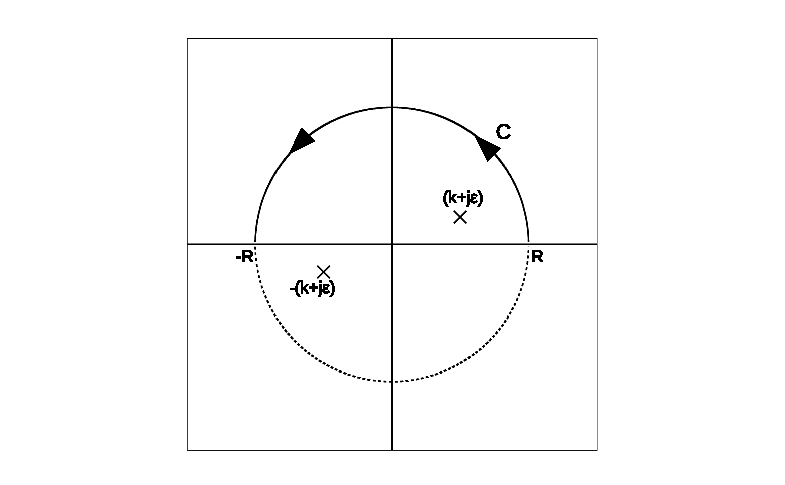
\includegraphics[width = 10cm]{./figure1new.eps}
    \label{fig1}
  \end{figure}
  \begin{eqnarray}
    F_+ = \int_{C} dk'\frac{e^{ik'(x-x')}}{(k'+k+i\epsilon)(k'-k-i\epsilon)} = \int_{-R}^Rdk' f_+(k') + \int_{C_1}dk'f_+(k')\label{c-int}
  \end{eqnarray}
  ただし
  \begin{eqnarray}
    f_+(k') = \frac{e^{ik'(x-x')}}{(k'+k+i\epsilon)(k'-k-i\epsilon)}
  \end{eqnarray}
  ここで留数定理
  \begin{eqnarray}
    \int_Cdz f(z) = 2\pi i\sum_j R(a_j)
  \end{eqnarray}
  を用いる. 極を$a_j$, Laurent展開における$(z-a)^{-n}$の係数を$R(a)$としている.今回の積分には1位の極しか含まれていないのでLaurent展開は
  \begin{eqnarray}
    R(a) = \lim_{z \rightarrow a}(z-a)f(z)
  \end{eqnarray}
  で与えられる. 以上より, (\ref{c-int})は
  \begin{eqnarray}
    F_+ &=& 2\pi i\lim_{k' \rightarrow k + j\epsilon }\left[(k'-k-j\epsilon)\frac{e^{ik'(x-x')}}{(k'+k+i\epsilon)(k'-k-i\epsilon)}\right]\\
    &=& \pi i\frac{e^{i(x-x')(k+j\epsilon)}}{k+j\epsilon}
  \end{eqnarray}
  と計算できる. さらに
  \begin{eqnarray}
    \lim_{R\rightarrow\infty}\int_{C_1}dk'f_+(k') =0
  \end{eqnarray}
  であることはすぐにわかる. 以上から
  \begin{eqnarray}
    G^\epsilon_+(x, x') &=& -\frac{1}{2\pi}\pi i\frac{e^{i(x-x')(k+j\epsilon)}}{k+j\epsilon}\\
    \therefore G_+(x, x') &=& \lim_{\epsilon\rightarrow 0}G_+^\epsilon(x, x') = -\frac{i}{2k}e^{ik(x-x')}
  \end{eqnarray}
  のように, Green関数を具体的に計算できた.\\
\item[ii)] $x<x'$の場合    
  \begin{figure}[htbp]
    \centering
    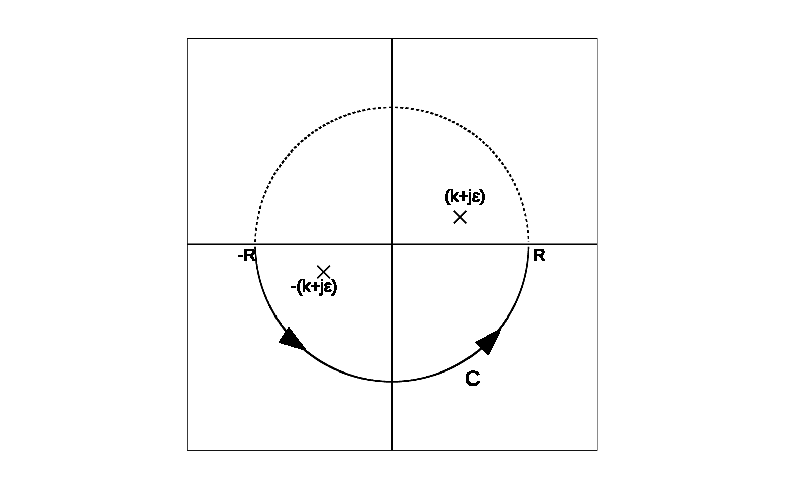
\includegraphics[width = 10cm]{./figure2new.eps}
    \label{fig2}
  \end{figure}
  先程と同様の計算より,
  \begin{eqnarray}
    G_-(x, x') = -\frac{i}{2k}e^{-ik(x-x')}
  \end{eqnarray}
  となる. 
\end{itemize}
まとめると,
\begin{eqnarray}
  G_\pm(x, x') = -\frac{i}{2k}e^{\pm ik(x-x')}
\end{eqnarray}
グリーン関数が求まったので, これを用いて波動関数を求める. 波動関数の摂動展開は
\begin{eqnarray}
  \psi(x) = \psi_0(x) + \int dx'G_+(x, x')H_p(x')\psi(x')
\end{eqnarray}
と表される.$\psi_0(x)$は非摂動解なので平面波であり, $H_p$はポテンシャルである. つまり, 領域ごとに$H_p$を変えてこの積分を計算すれば良い.
\section{場の理論におけるGreen関数}
場の理論と書きましたが, 以下では第二量子化された量子力学\footnote{「第二量子化された量子力学」と「場の量子論」は明確に区別されるべきです. 量子力学はあくまでSchr\"odinger方程式によって真空(基底状態)が決まるが, 場の量子論では真空は理論を閉じるように選ぶものである. 第二量子化における真空は消滅演算子$a$が消去する状態で確定しますが, 場の量子論においては真空期待値$\bra{0}\psi\ket{0}$がゼロでない値を持つことが許されます. こういう構造がないと, 粒子が存在する状態を真空とするBECのような物理を記述できなくなります.}におけるGreen関数についてまとめます.
\subsection{時間依存自由粒子Green関数}
場の演算子$\psi(\bm{x}, t)$はSchr\"odinger方程式
\begin{eqnarray}
  \left(i\hbar\partial_t -H\right)\psi(\bm{x}, t) = 0
\end{eqnarray}
で記述される. 今までの1粒子波動関数と同様に, 非摂動部のGreen演算子は
\begin{eqnarray}
  G_0(\bm{x}, t) = \left(i\hbar\partial_t -H_0\right)^{-1}
\end{eqnarray}
と表せ, グリーン関数は
\begin{eqnarray}
  \left(i\hbar\partial_t -H_0\right)G_0(\bm{x}, \bm{x}'; t, t') = \delta(t-t')\delta(\bm{x} - \bm{x}')
\end{eqnarray}
である. この微分方程式の解は2つ存在する:
\begin{eqnarray}
  G_0^R(k, \tau) &=& -i\theta(\tau)e^{-iE_k\tau}\hspace{1cm}\tau = t-t'\\
  G_0^A(k, \tau) &=& i\theta(\tau)e^{-iE_k\tau}\hspace{1cm}\tau = t'-t
\end{eqnarray}
$G^R$を遅延グリーン関数, $G^A$を先進グリーン関数と呼ぶ. 現象が時間に対して未来に進むのが遅延グリーン関数, 過去に進むのが先進グリーン関数になっている\footnote{数学的には時間が反転するような解を持っていてもおかしくないし, むしろ持っているべき. 時間発展がユニタリーなら解は時間反転対称性がある. }. 因果律を考慮しなくて良い場合であればどちらを用いてもよいが, 遅延グリーン関数の方が物理的な直感と合致している.
\subsection{相関関数と温度Green関数}
系が熱平衡状態にあるとき, $t = 0$の基底状態$\ket{\psi(0)}$を用いてGreen関数は, 可観測量$A, B$の時間相関関数で与えられる\footnote{Green関数が系に何かしらの揺動を与えた時の応答と解釈するなら自然な定義と言える.}:
\begin{eqnarray}
  G(t-t') \equiv \expval{\expval{A(t)B(t')}} = -i\bra{\psi(0)}{\rm T}[A(t)B(t')]\ket{0}
\end{eqnarray}
$A(t), B(t')$はHeisenberg描像, ${\rm T}[\ ]$は時間順序積. T積は因果律を守るために導入されている.

有限温度系における期待値は
\begin{eqnarray}
  \expval{A} = \frac{{\rm Tr}Ae^{-\beta H}}{{\rm Tr}e^{-\beta H}}
\end{eqnarray}
で与えられるので, 上のGreen関数は
\begin{eqnarray}
  G(t-t') &=& -i\frac{{\rm T}[{\rm Tr}A(t)B(t')e^{-\beta H}]}{{\rm Tr}e^{-\beta H}}\\
  &=& -i\frac{{\rm T}[{\rm Tr}e^{iHt/\hbar}Ae^{-iHt/\hbar}e^{iHt/\hbar}Be^{-iHt/\hbar}e^{-\beta H}]}{{\rm Tr}e^{-\beta H}}\\
  &=& -i\frac{{\rm T}[{\rm Tr}e^{iHt/\hbar}ABe^{-(it/\hbar + \beta)H}]}{{\rm Tr}e^{-\beta H}}
\end{eqnarray}
これを温度Green関数(松原Green関数)と呼ぶ.
\newpage
\chapter{超伝導}
超伝導の現象論であるGinzburg-Landau理論とBCS理論を扱う. 
\section{超電導の基礎}
\subsection{超電導体の性質}
\begin{itemize}
\item 電気抵抗ゼロ
\item 磁束の侵入を許さない (flux exclusion)
\item 磁束の排除が起こる (flux expulsion)
\end{itemize}
超伝導でない抵抗ゼロの金属ではflux expulsionはない.
\subsection{磁束の量子化}
磁束の量子化は超伝導の巨視波動関数$\psi = \psi_0e^{i\theta}$の一価性の要請から導かれる.
\begin{eqnarray}
  \nonumber  \bm{J}_s &=& \frac{e}{2m}\frac{\hbar}{i}(\psi^*\nabla) - \frac{e^2}{m}|\psi|^2\bm{A}\\
  &=& -\frac{e}{m}|\psi|^2(\hbar\nabla\theta + e\bm{A})
\end{eqnarray}
$\bm{J}_s ~ n_se\bm{v}_s = |\psi|^2e\bm{v}_s$であることに着目すると
\begin{eqnarray}
  \nabla\theta = -\frac{m}{\hbar}\bm{v}_s - \frac{e}{\hbar}\bm{A}
\end{eqnarray}
となる. 波動関数の一価性が保証されるには, 閉曲面$C$に沿って線積分したものが$2\pi$の整数倍でなければならない:
\begin{eqnarray}
  \int_C dl \nabla\theta = \int_C dl \bm{v}_s = 2\pi n
\end{eqnarray}
循環が量子化されている.
\section{超伝導の現象論 : Ginzburg-Landau理論}
超伝導を現象論的にモデル化したGinzburg-Landau理論について. 
\subsection{相転移とOder parameter}
ハミルトニアンが
\begin{eqnarray}
  H = -2\sum_{i,j}J\bm{s}_i\cdot\bm{s}_j
\end{eqnarray}
と書けるようなスピン相互作用を考える. これをハイゼンベルグ模型という. 系の平衡状態はHelmholtz自由エネルギー
\begin{eqnarray}
  F = U -TS
\end{eqnarray}
を最小にするように決まる. 低温($T<\!<U/S$)ならば内部エネルギー$U=\expval{H}$がleadingであり, これを最小化するようにスピンの向きが揃う. これを強磁性体と呼ぶ.  一方で高温ならばエントロピーの項が優勢なのでエントロピーが最大になるようにスピンの向きがバラバラになる. これを常磁性体と呼ぶ.

スピンの向きが揃うときに真空期待値が値を持ち, これを秩序変数と呼ぶ. 秩序変数がゼロでない値に変化するとき, これを相転移と呼ぶ.
\subsection{Ginzburg-Landau方程式}
自由エネルギーを秩序変数$\psi$の冪で展開:
\begin{eqnarray}
  {\cal F}[\psi] = {\cal F}_0 + \alpha|\psi|^2 + \frac{\beta}{2}|\psi|^4
\end{eqnarray}
ここで$\alpha = a(T-T_C)$である. 自由エネルギーの最小を与える$|\psi|$は微分すれば
\begin{eqnarray}
  |\psi| =
  \begin{cases}
    \hspace{1cm}0&(T>T_C)\\
    \\
    \sqrt{\cfrac{a(T_C-T)}{\beta}}&(T<T_C)
  \end{cases}
\end{eqnarray}
と求められる. そもそも$|\psi| = M$(磁化)と考えるのが自然で, なおかつ時間反転対称性を持っているので$M$の奇数次はない. $\alpha<0$のときに$|\psi| = 0$以外の極値を持つようになる. $\alpha(T) = a(T-T_C)$とすれば相転移を記述できる.

$\psi$が空間一様でない, つまり$\psi$が$r$依存性を持つ場合は
\begin{eqnarray}
  {\cal F} &=& {\cal F}_0 + \int d\bm{r} f(\bm{r})\\
  &=& {\cal F}_0 + \int dV\left[\alpha|\psi(\bm{r})|^2 + \frac{\beta}{2}|\psi(\bm{r})|^4\right]  
\end{eqnarray}
と書くことにする. 外部磁場などがある場合, 粒子の運動エネルギ^による補正項を加えなければならない:
\begin{eqnarray}
  \int dV \frac{\hbar^2}{2m}|\nabla\psi(\bm{r})|^2
\end{eqnarray}
自由エネルギーにはゲージ対称性があるので, ゲージ変換に対して不変な形で導入しなければならない:
\begin{eqnarray}
  {\cal F} &=& {\cal F}_0 + \int dV\left[\frac{\hbar^2}{2m}\left|\left(\nabla - \frac{ie}{\hbar}\bm{A}(\bm{r}))\psi(\bm{r}\right)\right|^2 + \alpha|\psi(\bm{r})|^2 + \frac{\beta}{2}|\psi(\bm{r})|^4 + \frac{\mu_0}{2}(\nabla\times\bm{A})^2\right]
\end{eqnarray}
これの変分がゼロになるところを探す:
\begin{eqnarray}
  \nonumber  \delta{\cal F} &=&\int dV\left[-\frac{\hbar^2}{2m}\left(\nabla - \frac{ie}{\hbar}\bm{A}(\bm{r})\right)^2\psi(\bm{r}) + \alpha\psi(\bm{r}) + \beta|\psi(\bm{r})|^2\psi(\bm{r})\right]\delta\psi^*(\bm{r})\\
  &+&\int \left[\frac{\hbar^2}{2m}\left(\nabla - \frac{ie}{\hbar}\bm{A}(\bm{r})\right)\psi(\bm{r})\right]\delta\psi^*(\bm{r})\cdot d\bm{S}
\end{eqnarray}
右辺第一項の被積分関数がゼロになることから
\begin{eqnarray}
  \left[-\frac{\hbar^2}{2m}\left(\nabla - \frac{ie}{\hbar}\bm{A}(\bm{r})\right)^2 + \alpha + \beta|\psi(\bm{r})|^2\right]\psi(\bm{r}) = 0\label{GL}
\end{eqnarray}
を得る. これが秩序変数を記述するGinzburg-Landau(GL)方程式である. ちなみに今回は${\cal F}$について$\psi$の変分を取ったが, $A$についての変分を取るとアンペールの法則が出てくる.
\subsection{ゲージ変換の復習}
\subsubsection{Maxwell方程式}
電磁気学におけるゲージ変換のおはなし. Maxwell方程式
\begin{eqnarray}
  {\rm rot} \bm{E} + \frac{\partial\bm{B}}{\partial t} &=& 0\hspace{2cm}(ファラデーの法則)\\
  {\rm rot} \bm{B} - \varepsilon_0\mu_0\frac{\partial \bm{E}}{\partial t} &=& \mu_0 \bm{i}\hspace{2cm}(アンペールの法則)\\
  {\rm div} \bm{E} &=& \frac{\rho}{\varepsilon_0}\hspace{2cm}(電荷のガウスの法則)\\
  {\rm div} \bm{B} &=& 0\hspace{2cm}(電荷のガウスの法則)
\end{eqnarray}
について. $\bm{B} = {\rm rot}\bm{A}$という仮定をすると${\rm div}\bm{B} = {\rm div\ rot}\bm{A} = 0$という関係が自明に出てくる(ただし, これは$\bm{A}$に特異点がない場合). この仮定をファラデーの法則に代入:
\begin{eqnarray}
  {\rm rot}(\bm{E} + \frac{\partial \bm{A}}{\partial t}) = 0
\end{eqnarray}
もし
\begin{eqnarray}
  \bm{E} + \frac{\partial \bm{A}}{\partial t} = -{\rm grad}\phi \hspace{0.5cm}\Longrightarrow\hspace{0.5cm} \bm{E} = -{\rm grad}\phi - \frac{\partial \bm{A}}{\partial t}
\end{eqnarray}
という仮定をすればファラデーの法則も自明となる. $\phi$と$A$が導入できればMaxwell方程式がとてもカンタンになる. $\phi$と$A$をまとめて電磁ポテンシャルと呼ぶ. 新しい方程式は
\begin{eqnarray}
  \left(\nabla^2 - \varepsilon_0\mu_0\frac{\partial^2}{\partial t^2}\right)\bm{A} - {\rm grad}\left({\rm div}\bm{A} + \varepsilon_0\mu_0\frac{\partial \phi}{\partial t}\right) &=& -\mu_0\bm{i}\label{max1}\\
  \nabla^2\phi + {\rm div}\frac{\partial \bm{A}}{\partial t} &=& -\frac{\rho}{\varepsilon_0}\label{max2}
\end{eqnarray}
となる.ここで
\begin{eqnarray}
  \bm{A}' = \bm{A} + {\rm grad}\chi
\end{eqnarray}
という量を定義しても, 磁束密度$\bm{B}$は変わらない. その代わり電場は変わってしまうので
\begin{eqnarray}
  \phi' = \phi - \frac{\partial \chi}{\partial t}
\end{eqnarray}
を導入すると全て辻褄が合う. この$(\phi, \bm{A})\mapsto(\phi', \bm{A}')$の変換をゲージ変換と呼び, Maxwell方程式はゲージ不変性を持つ.
\subsubsection{ローレンツゲージ}
(\ref{max1})(\ref{max2})には各々$\phi, \bm{A}$が含まれているので計算がめんどくさい. せめて
\begin{eqnarray}
  {\rm div}\bm{A} + \varepsilon_0\mu_0\frac{\partial \phi}{\partial t} = 0\label{max3}
\end{eqnarray}
となってくれれば(\ref{max1})は
\begin{eqnarray}
  \left(\nabla^2 - \varepsilon_0\mu_0\frac{\partial \phi}{\partial t}\right)\bm{A} = -\mu_0\bm{i}\label{max4}
\end{eqnarray}
のように$\bm{A}$だけの式になり, (\ref{max3})を(\ref{max2})に代入すると
\begin{eqnarray}
  \left(\nabla^2 - \varepsilon_0\mu_0\frac{\partial^2}{\partial t^2}\right)\phi &=& -\frac{\rho}{\varepsilon_0}
\end{eqnarray}
という対称性のとてもよい形になる. (\ref{max3})をローレンツ条件という.
\begin{itembox}[c]{ローレンツゲージにおけるMaxwell方程式}
  \begin{eqnarray}
    \nonumber    \left(\nabla^2 - \varepsilon_0\mu_0\frac{\partial \phi}{\partial t}\right)\bm{A} &=& -\mu_0\bm{i}\\
    \nonumber    \left(\nabla^2 - \varepsilon_0\mu_0\frac{\partial^2}{\partial t^2}\right)\phi &=& -\frac{\rho}{\varepsilon_0}
  \end{eqnarray}
  ただし
  \begin{eqnarray}
    \nonumber    {\rm div}\bm{A} + \varepsilon_0\mu_0\frac{\partial \phi}{\partial t} = 0
  \end{eqnarray}
\end{itembox}
\begin{eqnarray}
  (\phi, \bm{A})\mapsto(\phi', \bm{A}') \Longrightarrow
  \begin{cases}
    \bm{A}' = \bm{A} + {\rm grad}\chi\\
    \phi' = \phi - \cfrac{\partial \chi}{\partial t}
  \end{cases}
\end{eqnarray}

がローレンツ条件(\ref{max3})を満たすような$\chi$が存在すれば, この以上の変形が正当化される. ローレンツゲージによるMaaxwell方程式はローレンツ共変である. 
\subsubsection{クーロンゲージ}
ローレンツ条件に対して
\begin{eqnarray}
  {\rm div}\bm{A} = 0
\end{eqnarray}
という条件を課すと, クーロンの法則と等価なポアソン方程式が導かれることからこれをクーロン条件(クーロンゲージ)と呼ぶ.
\begin{itembox}[c]{クーロンゲージにおけるMaxwell方程式}
  \begin{eqnarray}
    \nonumber   && \nabla^2\phi = -\frac{\rho}{\varepsilon_0}\\
    \nonumber    &&\nabla^2\bm{A} -\varepsilon_0\mu_0\frac{\partial^2 \bm{A}}{\partial t^2} - \varepsilon_0\mu_0\frac{\partial}{\partial t}{\rm grad}\phi = \mu_0\bm{i}
  \end{eqnarray}
  ただし
  \begin{eqnarray}
    \nonumber    {\rm div}\bm{A} = 0
  \end{eqnarray}
\end{itembox}
クーロンゲージはローレンツ共変ではなくあまり方程式の対称性は良くないが, 電磁場の量子化などでは便利なので用いられることがある.
\subsection{GLコヒーレンス長と侵入長}
外部磁場がない場合の一次元GL方程式(\ref{GL})を境界条件$\psi(0) = 0$のもとで解く:
\begin{eqnarray}
  \left[-\frac{\hbar^2}{2m}\frac{d^2}{dx^2} + \alpha + \beta|\psi(x)|^2\right]\psi(x) = 0  
\end{eqnarray}
これは$x = 0$の境界には超伝導体はなく, $x > 0$を超電導体で占められているような状況である. コヒーレンス長$/xi$を
\begin{eqnarray}
  \xi^2 = \frac{\hbar^2}{2m|\alpha|}
\end{eqnarray}
と定義する. 超伝導状態では$\alpha < 0$である\footnote{こうしないとGLヘルムホルツエネルギーが$\psi>0$の領域で最小値を持たなくなる.}. 両辺を$\psi_0 = \sqrt{|\alpha|/\beta}$を用いて整理して
\begin{eqnarray}
  -\frac{d^2\psi}{dx^2} - \psi + \psi^3 = 0
\end{eqnarray}
を得る. 左辺に$2\frac{d\psi}{dx}$を掛ける:
\begin{eqnarray}
  2\frac{d\psi}{dx}\left[-\frac{d^2\psi}{dx^2} - \psi + \psi^3\right] = 0
\end{eqnarray}
ここで
\begin{eqnarray}
  \frac{d}{dx}\left(\frac{d\psi}{dx}\right)^2 = 2\frac{d\psi}{dx}\left(\frac{d^2\psi}{dx^2}\right), \hspace{0.5cm}\frac{d\psi^2}{dx} = 2\psi\frac{d\psi}{dx}, \hspace{0.5cm}\frac{d\psi^4}{dx} &=& 4\psi^3\frac{d\psi}{dx}
\end{eqnarray}
を用いて変形する:
\begin{eqnarray}
  \frac{d}{dx}\left[-\xi^2\left(\frac{d\psi}{dx}\right)^2-\psi^2 + \frac{1}{2}\psi^4\right] = 0
\end{eqnarray}
微分がゼロなので微微分関数は定数:
\begin{eqnarray}
  -\xi^2\left(\frac{d\psi}{dx}\right)^2-\psi^2 + \frac{1}{2}\psi^4 = A\ ({\rm const})
\end{eqnarray}
また, 境界条件$d\psi/dx\rightarrow 0, \psi\rightarrow 1\ (x\rightarrow+\infty)$を課すと$A = -\frac{1}{2}$であることがわかる. これにより
\begin{eqnarray}
  \xi^2\left(\frac{d\psi}{dx}\right)^2 = \frac{1}{2}\left(1-\psi^2\right)
\end{eqnarray}
という方程式が得られる.

これは非線形微分方程式だが特解を持っている:
\begin{eqnarray}
  \psi(x) = \tanh(\frac{x}{\sqrt{2\xi}})
\end{eqnarray}
これはソリトン解と呼ばれる. $x = 0$で強制的にゼロにされた$\psi$が$\xi$程度で回復している.また
\begin{eqnarray}
  \xi = \left(\frac{\hbar^2}{2m|\alpha|}\right)^{\frac{1}{2}} = \left(\frac{\hbar^2}{2ma(T-T_C)}\right)^{\frac{1}{2}} = \left(\frac{\hbar^2}{2maT_C}\right)^{\frac{1}{2}}\left(1 - \frac{T}{T_C}\right)^{\frac{1}{2}}
\end{eqnarray}
$T\rightarrow T_C\ (T_C > T)$でコヒーレンス長は発散していく自然な結果が得られる.
\subsection{ソリトンの特徴}
普通の線形波なら波動方程式で記述される異なる波長を持つ波の重ね合わせで記述できる. 異なる波長の波は$v = f\lambda$に従って伝搬速度も異なるので, 波束は次第に崩壊していく(分散が発散していく). しかしソリトンはある非線形微分方程式の定常解なので形を変えずに伝搬していき, 波束も崩壊しない.
\section{超伝導の微視的理論 : Bardeen-Cooper-Schrieffer理論}
\subsection{金属の基本性質}
一辺$L$の箱に閉じ込められた自由電子について考える. 周期境界条件を課すと, 波動関数は平面波で記述できる:
\begin{eqnarray}
  \psi_{\bm{k}}(\bm{r}) = \frac{1}{\sqrt{L^3}}e^{i\bm{k}\cdot\bm{r}}
\end{eqnarray}
エネルギー分散関係は
\begin{eqnarray}
  \varepsilon_{\bm k} = \frac{\hbar^2k^2}{2m}
\end{eqnarray}
である. ここで波数は
\begin{eqnarray}
  k_i = n_i\left(\frac{2\pi}{L}\right)\hspace{0.5cm}(i= x, y, z)
\end{eqnarray}
で与えられる. 3次元$k$空間の単位体積$(2\pi/L)^3$あたりに1つ(スピン自由度を考えると2つ)の状態が入れる. 下の準位から埋めていくと, 状態が埋まった空間は球になる. これをフェルミ球と呼び, その境界をフェルミ面と呼ぶ. フェルミ面の半径を$k_F$とすると
\begin{eqnarray}
  N = 2\left(\frac{L}{2\pi}\right)^3\times\frac{4}{3}\pi k_F^3
\end{eqnarray}
である. 電子密度を$n = N/L^3$とすると
\begin{eqnarray}
  k_F = (3\pi n)^{\frac{1}{3}}
\end{eqnarray}
となる. エネルギー$\varepsilon$の状態を電子が占める確率はFermi-Dirac分布関数
\begin{eqnarray}
  f(\varepsilon) = \frac{1}{\exp[(\varepsilon- \varepsilon_F)/k_BT]+1}
\end{eqnarray}
で与えられる.
\subsection{電子-格子間相互作用}
電子と金属イオンの間の相互作用は電子がイオン構造を歪めるという描像で理解される\footnote{金属イオン中に電子があると電子と金属イオンが引力相互作用で近づき合い, 金属イオンの配列が微妙に歪むことになる. この電子が金属中を移動すると, 金属イオンの配列の歪みも一緒に伝搬していくように見える. これが格子振動であり, これを量子化するとフォノンになる. さて, この場合は電子の運動エネルギーが格子振動に一部持って行かれることになり, これが電気抵抗の由来になる. しかし, この電子の近くに別の電子がある場合は, 格子振動により正電荷密度が大きくなっているところからさらに引力相互作用を受けて加速することができる. つまり, ある電子が創りだした格子振動エネルギーを別の電子が受け取る, というメカニズムである. もちろんこれば古典的な描像であり, 全ての格子振動エネルギーが別の電子に引き継がれることは一見なさそうだが, 格子振動を量子化したフォノンであればdescreteなエネルギーのやりとりしかできないことになるので, 電子がフォノンのやりとりをすることでエネルギーの散逸を防ぐ枠組みを正当化することができそうである. このフォノンのやり取りをする電子の組をCooper-pairという. }. つまり, 電子がフォノンを放出して異なる波数を持つモードへ遷移する, という描像である. フォノンを介した2電子間相互作用とは, 波数$k_1, k_2$の電子が$k_1 - q, k_2 + q$となる過程である.

\begin{figure}[htbp]
  \begin{minipage}{0.5\hsize}
    \centering
    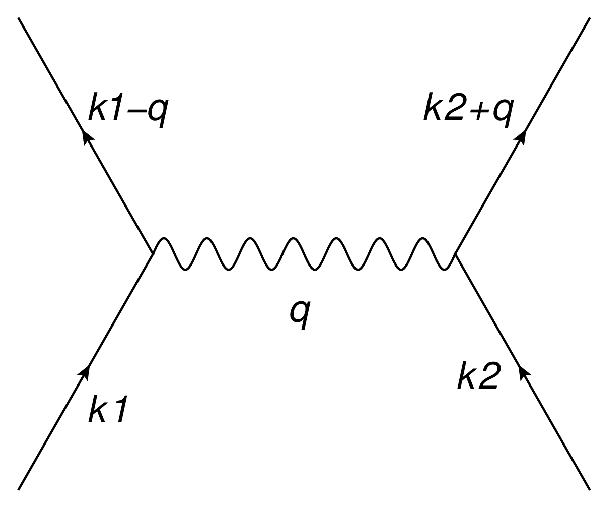
\includegraphics[width = 5.5cm]{./newdiagram1.eps}
    \figcaption{$\bm{k}_1$がフォノン$\bm{q}$を放出する過程}
    \label{diagram1}
  \end{minipage}
  \begin{minipage}{0.5\hsize}
    \centering
    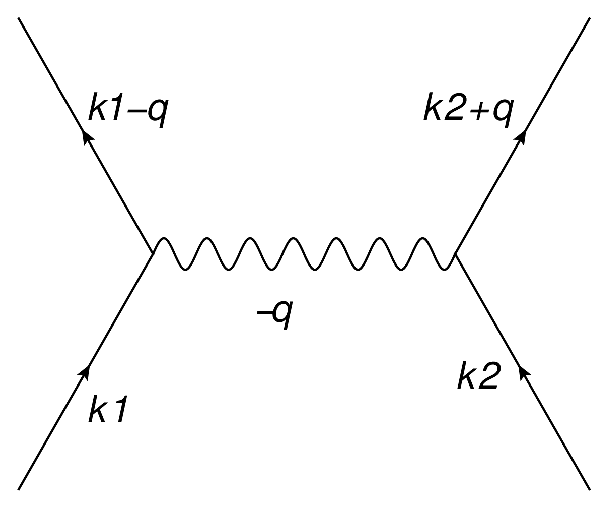
\includegraphics[width = 5.5cm]{./newdiagram2.eps}
    \figcaption{$\bm{k}_1$がフォノン$\bm{-q}$を吸収する過程}
    \label{diagram2}
  \end{minipage}
\end{figure}
フォノンを介した相互作用ハミルトニアンを$H'$とすると, エネルギーの2次摂動は
\begin{itemize}
\item 同じ電子がフォノンを放出して吸収した場合は自己エネルギー
\item 異なる電子同士がフォノンのやりとりをした場合は相互作用
\end{itemize}
を表すことになる. さて, 上の2種類の過程を考慮すると相互作用項の期待値は
\begin{eqnarray}
  U_2 &=& \sum_m\frac{\bra{f}H'\ket{m}\bra{m}H'\ket{i}}{E_i-E_m}\\
  E_i &=& \varepsilon_{\bm{k}_1} +\varepsilon_{\bm{k}_2}\\
  E_m &=&
  \begin{cases}
    \varepsilon_{\bm{k}_1 - \bm{q}} +\varepsilon_{\bm{k}_2} + \hbar\omega_{\bm{q}}\\
    \varepsilon_{\bm{k}_1} +\varepsilon_{\bm{k}_2 + \bm{q}} + \hbar\omega_{\bm{q}}
  \end{cases}
\end{eqnarray}
より
\begin{eqnarray}
  U_2 &=& \frac{|V_{\bm q}|^2}{\varepsilon_{\bm{k}_1 - \bm{q}} +\varepsilon_{\bm{k}_1} + \hbar\omega_{\bm{q}}} + \frac{|V_{\bm q}|^2}{\varepsilon_{\bm{k}_2} +\varepsilon_{\bm{k}_2 + \bm{q}} + \hbar\omega_{\bm{q}}}\\
  &=& \frac{2|V_{\bm q}|\hbar\omega_{\bm q}}{(\varepsilon_{\bm{k}_1 - \bm{q}} +\varepsilon_{\bm{k}_1})^2-(\hbar\omega_{\bm q})^2}
\end{eqnarray}
となる. ここではエネルギー保存則を用いた. $|\varepsilon_{\bm k} - \varepsilon_{\bm k-q}| <\!< \hbar\omega_{\bm q}$であれば電子間相互作用は引力となる. つまり, フェルミ面上の電子間にはフォノンを介した引力相互作用が働く可能性がある.
\subsection{Cooper問題}
次に問題になるのが, 「フェルミ面直上にある2つの電子間相互作用を考えるとき, この電子対が束縛状態を作るか」ということ. 言い換えると, 「いかに弱くても引力相互作用があれば電子対の束縛状態が実現するかどうか」. 着目する2電子の波動関数を
\begin{eqnarray}
  \Psi(\bm{r}_1, \sigma_1, \bm{r}_2, \sigma_2) = \psi(\bm{r}_1, \bm{r}_2)\chi(\sigma_1, \sigma_2)
\end{eqnarray}
とする. $\psi$が満たすのはScr\"odinger方程式
\begin{eqnarray}
  &&\bqty{-\frac{\hbar^2}{2m}\pqty{\nabla^2_1 + \nabla^2_2} + V(\bm{r}_1, \bm{r}_2)}\psi(\bm{r}_1, \bm{r}_2) = E\psi(\bm{r}_1, \bm{r}_2)\\
  &&\chi(\sigma_1, \sigma_2) = \frac{1}{\sqrt{2}}\pqty{\ket{\uparrow}\ket{\downarrow} - \ket{\downarrow}\ket{\uparrow}}
\end{eqnarray}
重心・相対座標$\bm{R} = \pqty{\bm{r}+\bm{r}}/2,\ \bm{r} = \bm{r}_1 - \bm{r}_2$を用いて
\begin{eqnarray}
  \psi(\bm{r}_1,\bm{r}_2) = \varphi(\bm{r})e^{i\bm{KR}}
\end{eqnarray}
\newpage
\chapter{熱・統計力学}
\section{熱力学}
\subsection{状態量}
系の状態のみで一意に決まり, 過去の履歴・経路に依らない(積分値が経路に依らない)ものを状態量と呼ぶ. 
\subsection{完全な熱力学関数}
系の平衡状態における熱力学的性質の情報を全て持っているものを完全な熱力学関数と呼ぶ. 示量性状態量. 系の情報を全て持っているというのは, 状態量がこの関数の偏微分で全て求まるということ. 例えば内部エネルギー$U(S, N, V)$を用いて
\begin{eqnarray}
  \partial_SU &=& T\\
  \partial_NU &=& \mu\\
  \partial_VU &=& -p
\end{eqnarray}
という状態量が求まる. 全微分は
\begin{eqnarray}
  dU = TdS -pdV + \mu dN
\end{eqnarray}
である. これを変形して
\begin{eqnarray}
  dS = \frac{1}{T}dU +\frac{p}{T}dV - \frac{\mu}{T} dN
\end{eqnarray}
となり, $S$は$U, V, N$を変数とする関数として表された時に完全な熱力学関数となる. 統計力学においては温度を定義するときに
\begin{eqnarray}
  \partial_US = \frac{1}{T}
\end{eqnarray}
という表式をしばしば用いる.
\subsection{自由エネルギー}
熱力学第二法則より, 系は自由エネルギーが減少する方向に遷移する. 
\subsubsection{ヘルムホルツ自由エネルギー}
等温下で仕事として取り出し可能なエネルギーを表す.ヘルムホルツエネルギーが極小値を取るとき, 系は熱平衡状態にある.

定義:
\begin{eqnarray}
  F(T, V, N) = U(S(T, V, N), V, N) -TS(T, V, N)
\end{eqnarray}
ここで現れるエントロピーは完全な熱力学関数ではない. 各変数による偏微分は
\begin{eqnarray}
  \partial_TF &=& -S\\
  \partial_VF &=& -p\\
  \partial_NF &=& \mu
\end{eqnarray}
である. 全微分は
\begin{eqnarray}
  dF = -S(T, V, N)dT -p(T, V, N)dV + \mu(T, V, N) dN
\end{eqnarray}
\subsubsection{ギブズ自由エネルギー}
等温等圧下で仕事として取り出し可能なエネルギーを表す. ヘルムホルツエネルギーとの違いは等圧条件の有無.

定義:
\begin{eqnarray}
  G(T, p, N) = U(S(T, p, N), p, N) -TS(T, p, N)
\end{eqnarray}
以下ヘルムホルツエネルギーと同様.
\section{統計力学}
\subsection{目的}
微視的状態の数をかぞえて巨視的状態を導く. 
\subsection{ミクロカノニカルアンサンブル}
\subsection{Langevin方程式}
ブラウン粒子の運動を記述する方程式としてLangevinが導入した.
\begin{eqnarray}
  M\frac{dv}{dt} = -\frac{v}{\mu} + F_{\rm ext} + R(t)\label{Langevin}
\end{eqnarray}
ここで$\mu$を移動度, $F_{ext}$をマクロな外力, $R(t)$をミクロなノイズとする. $R$が確率過程であるので, 初期条件を与えても$v$が決定論的に定まらない. 

速度をFourier変換する:
\begin{eqnarray}
  v(t) &=& \frac{1}{\sqrt{2\pi}}\int d\omega e^{-i\omega t}\tilde{v}(\omega)\label{v1}\\
  \tilde{v}(\omega) &=& \frac{1}{\sqrt{2\pi}}\int dt e^{i\omega t}v(t)\label{v2}
\end{eqnarray}
さらに速度の時間相関関数とそのFourier変換を定義する:
\begin{eqnarray}
  C_v(t) &=& \expval{v(t_0)v(t_0 + t)}\\
  \tilde{C}_v(\omega) &=& \frac{1}{\sqrt{2\pi}}\int dt'e^{i\omega't'}\expval{v(t_0)v(t_0+t')}
\end{eqnarray}
ここで$\tilde{v}^*(\omega) = \tilde{v}(-\omega)$が成立している. (\ref{v2})より
\begin{eqnarray}
  \expval{\tilde{v}(\omega)\tilde{v}^*(\omega')} &=& \frac{1}{2\pi}\int dtdt' e^{i\omega t-i\omega' t'}\expval{v(t)v(t')}\\
  &=&\frac{1}{2\pi}\int dtdt'\left|\det(J)\right| e^{i\omega t'}e^{i(\omega -\omega')t}\expval{v(t+t')v(t)}\\
  &=&\delta(\omega-\omega')\int dt'e^{i\omega' t'}\expval{v(t+t')v(t)}\\
  &=&\delta(\omega-\omega')I_v(\omega')
\end{eqnarray}
ただし
\begin{eqnarray}
  J =
  \begin{pmatrix}
    \cfrac{\partial(t+t')}{\partial t}&\cfrac{\partial(t+t')}{\partial t'}\\
    \cfrac{\partial t'}{\partial t}&\cfrac{\partial t'}{\partial t'}\\
  \end{pmatrix}\hspace{1cm} |\det(J)| = 1
\end{eqnarray}
である. この式から
\begin{eqnarray}
  I_v(\omega) = \int dtC_v(t)e^{i\omega t} = \tilde{C}(\omega)
\end{eqnarray}
がわかる. これをWiener-Khinchinの定理という. 相関関数とパワースペクトルはFourier変換を通して関係付けられる.$\tilde{R}(\omega)$についても同様のことが言える:
\begin{eqnarray}
  \tilde{R}(\omega) &=& \frac{1}{\sqrt{2\pi}}\int dt e^{i\omega t}R(t)\label{R2}\\
  \tilde{C}_R(\omega) &=& \frac{1}{\sqrt{2\pi}}\int dte^{i\omega t}\expval{R(t_0)R(t_0+t)}\\
  \expval{\tilde{R}(\omega)\tilde{R}^*(\omega')}&=& \tilde{C}_R(\omega')\delta(\omega-\omega') 
\end{eqnarray}

以降$F_{\rm ext} = 0$のもとでLangevin方程式の解析をする. (\ref{Langevin})に(\ref{v1})を代入:
\begin{eqnarray}
  M\frac{d}{dt}\int d\omega e^{-i\omega t}\tilde{v}(\omega) &=& \int d\omega e^{-i\omega t}\left(-\frac{\tilde{v}(\omega)}{\mu} + \tilde{R}(\omega)\right)  \\
  \Longleftrightarrow M(-i\omega)\tilde{v}(\omega) &=&  -\frac{\tilde{v}(\omega)}{\mu} + \tilde{R}(\omega)
\end{eqnarray}
$\gamma = (M\mu)^{-1}$とすると
\begin{eqnarray}
  \tilde{v}(\omega) = \frac{1}{-i\omega + \gamma}\frac{\tilde{R}(\omega)}{M}
\end{eqnarray}
であることがわかる. 時間相関関数は
\begin{eqnarray}
  \tilde{C}_v(\omega) &=& \int d\omega' \expval{\tilde{v}(\omega)\tilde{v}^*(\omega')} = \frac{1}{(-i\omega + \gamma)(i\omega' + \gamma)M^2}\int d\omega' \expval{R(\omega)R^*(\omega')}\\
  &=& \frac{1}{(-i\omega + \gamma)(i\omega' + \gamma)M^2}\int d\omega' \tilde{C}_R(\omega')\delta(\omega-\omega') = \frac{1}{\omega^2 + \gamma^2}\frac{\tilde{C}_R(\omega)}{M^2}
\end{eqnarray}
$R$の確率過程の性質が与えられてパワースペクトル$C_R$が定まると速度$v$の相関関数やパワースペクトルが決定される. $R$がホワイトノイズだと仮定すると,
\begin{eqnarray}
  C_R(t) = \expval{R(t_0+t)R(t_0)} = C_R\delta(t)\\
  \tilde{C}_R(\omega) = \int dt e^{-i\omega t}C_R(t) = C_R
\end{eqnarray}
ということで, $\tilde{C}_R$は$\omega$によらない定数になる. このようなノイズを仮定すると, 速度相関関数は
\begin{eqnarray}
  C_v(t) = \int d\omega e^{-i\omega t}\tilde{C}_v(\omega) = \int d\omega \frac{C_Re^{-i\omega t}}{M^2(\omega^2 + \gamma^2)}
\end{eqnarray}
この積分を実行するために複素積分の応用を用いる:
\begin{eqnarray}
  \int_C dz \frac{C_Re^{-izt}}{M^2(z^2 + \gamma^2)} = \int_{C_1} \frac{C_Re^{-izt}}{M^2(z^2 + \gamma^2)} + \int_{-R}^R \frac{C_Re^{-izt}}{M^2(z^2 + \gamma^2)}
\end{eqnarray}
\begin{figure}[htbp]
  \centering
  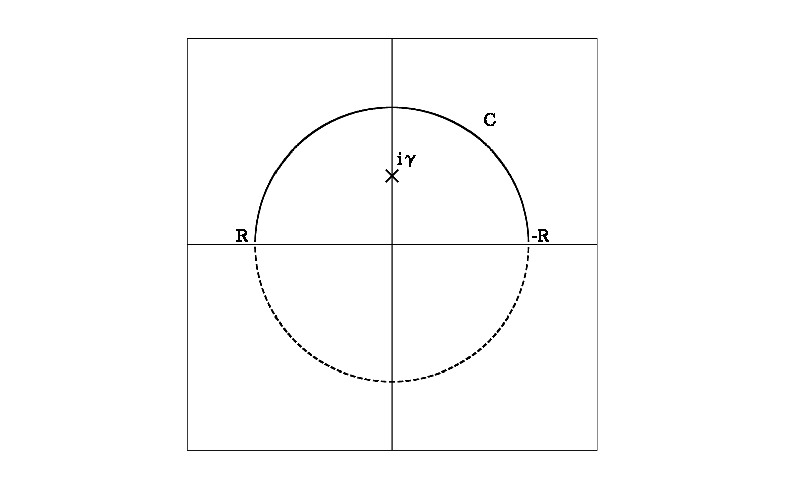
\includegraphics[width = 10cm]{./figure3new.eps}
  \label{fig3}
\end{figure}\\
極は$\omega = \pm i\gamma$で一位の極. 積分経路は上半円とする. 留数定理より
\begin{eqnarray}
  R(i\gamma) = \lim_{z\rightarrow i\gamma}(z - i\gamma)f(z) = \frac{C_Re^{\gamma t}}{2i\gamma}\label{R}
\end{eqnarray}
ここで$z = Re^{i\theta}$の変数変換を施すことにより
\begin{eqnarray}
  \int_{C_1}dz\frac{e^{-izt}}{(z^2 + \gamma^2)} = \int_0^\pi d\theta\frac{iRe^{-iRe^{i\theta}}t}{(R^2e^{2i\theta} + \gamma^2)}= \int_0^\pi d\theta\frac{iRe^{-iRt\cos\theta}e^{Rt\sin\theta}}{(R^2e^{2i\theta} + \gamma^2)}
\end{eqnarray}
かつ一般に$|\alpha + \beta| > |\alpha|-|\beta|$が成立することから
\begin{eqnarray}
  \left|\frac{iRe^{-iRt\cos\theta}e^{Rt\sin\theta}}{(R^2e^{2i\theta} + \gamma^2)}\right| < \frac{Re^{Rt\sin\theta}}{R^2 - \gamma^2}
\end{eqnarray}
これが$R\rightarrow\infty$で発散しないためには$t<0$である必要があるが, $t>0$の場合も発散しないようにしたい. そのためには$e^{-izt}\rightarrow e^{iz|t|}$とすればよい. つまり, (\ref{R})は
\begin{eqnarray}
  R(i\gamma) = \lim_{z\rightarrow i\gamma}(z - i\gamma)f(z) = \frac{C_Re^{-\gamma |t|}}{2i\gamma}\label{R2}
\end{eqnarray}
とするべきである. 以上からコーシーの積分定理より
\begin{eqnarray}
  C_v(t) = \frac{C_Re^{-\gamma|t|}}{2M^2\gamma}
\end{eqnarray}
となる. 同時刻($t = 0$)の相関は
\begin{eqnarray}
  C_v = \frac{C_R}{2M^2\gamma}
\end{eqnarray}
であり, 熱平衡状態のエネルギー等分配則
\begin{eqnarray}
  M\expval{v^2} = k_BT
\end{eqnarray}
を認めれば
\begin{eqnarray}
  C_R = 2k_BTM\gamma
\end{eqnarray}
となる. これはNyquistの定理と呼ばれ, 揺動散逸定理のひとつである.
\newpage
\chapter{量子統計力学}
\section{Born-Markov型量子マスター方程式}
熱浴と接している一次元調和振動子系のBorn-Markov型量子マスター方程式を解く.
\begin{itemize}
\item 系のハミルトニアンは調和振動子$H = \hbar\omega a^\dagger a$.
  
\item Born-Markov近似なので熱浴の密度演算子は時間発展せず, 回転波近似(弱結合)も有効.
  
\item マスター方程式は系の密度演算子の時間発展を与えている.\footnote{描像によっては生成消滅演算子も時間依存しそうである. 普通(?)マスター方程式を導出するときは相互作用描像を経由するので生成消滅演算子も一般に時間依存性を持つ. しかし今回は回転波近似が有効であるため, $a(t) = a(0)e^{-i\omega t}$のように分解できる. 後述のマスター方程式には$a^\dagger$, $a$がペアになって現れているので, マスター方程式には生成消滅演算子に依る時間依存性は現れない. $a^\dagger$, $a$がペアになっていないような項が現れたら生成消滅演算子由来の時間依存性を考慮しなければならないが, そもそもそういう項を落とすのがBorn-Markov近似である. }.
\end{itemize}
\begin{itemize}
\item 生成消滅演算子と粒子数状態
  
\item 交換関係の計算  
\end{itemize}
あたりの知識が必要です.
\subsection{問題設定}
量子マスター方程式が与えられている:
\begin{eqnarray}
  \nonumber  \partial_t\rho(t) = &-&i\omega[a^\dagger a, \rho(t)] + \kappa\overline{n}(2a^\dagger\rho(t)a - aa^\dagger\rho(t) - \rho(t)aa^\dagger)\\
  &+&\kappa(\overline{n} + 1)(2a\rho(t)a^\dagger - a^\dagger a\rho(t) - \rho(t)a^\dagger a)\label{master}
\end{eqnarray}
ただし
\begin{eqnarray}
  \kappa > 0,\hspace{1cm} \overline{n} = \frac{1}{e^{\hbar\omega/kT}-1},\hspace{1cm} [a, a^\dagger] = 1
\end{eqnarray}
であり, $\kappa$は減衰定数, $\overline{n}$はBose-Einstein分布関数, $a, a^\dagger$は生成消滅演算子である.
\subsection{熱平衡(問題1)}
熱浴の温度が$T$であることから, 系の温度を$T$とする有限温度系を考えればそれが熱平衡状態にあることは明らか. 平衡状態なので密度演算子が系のハミルトニアンを用いて
\begin{eqnarray}
  \rho_{th} = \frac{e^{-H/kT}}{{\rm Tr}e^{-H/kT}}\label{equiliblium}
\end{eqnarray}
と書ける. (\ref{equiliblium})の分母は規格化条件であり,以下のように計算できる\footnote{トレースは直行完全系ではさんで和を取ればいい.規格化は後でできるので, 正規直行完全系でなくてもいいらしい. つまりどんな完全系を選んできても規格化係数を除けば同じ結論に辿り着く. 今回は明らかに$a^\dagger a$の固有状態$\ket{n}$を用いるのが簡単. }(以下, 逆温度$1/kT$を$\beta$と置き換えています):
\begin{eqnarray}
  \nonumber  {\rm Tr}e^{-\beta\hbar\omega a^\dagger a} &=& \sum_{n}\bra{n}e^{-\beta\hbar\omega a^\dagger a}\ket{n}\\
  \nonumber  &=& \sum_{n}e^{-\beta\hbar\omega n}\\
  &=& \frac{1}{1-e^{-\beta\hbar\omega}} = (\overline{n} -1)
\end{eqnarray}

密度演算子はLiouville-von Neumann方程式を満たす:
\begin{eqnarray}
  i\hbar\partial_t\rho_{th} &=& [H, \rho_{th}]\\
  &=& \frac{\hbar\omega}{\overline{n}-1}[a^\dagger a, e^{\beta\hbar\omega a^\dagger a}]\label{commutation}
\end{eqnarray}
$[A, [B, A]] = [B, [B, A]] = 0$が成立しているときに$[B, e^{\lambda A}] = \lambda[B, A]e^{\lambda A}$であることを利用して\footnote{証明してみよう!}
\begin{eqnarray}
  (\ref{commutation}) = \frac{\hbar\omega}{\overline{n}-1}\beta\hbar\omega[a^\dagger a, a^\dagger a]e^{\beta\hbar\omega a^\dagger a} = 0
\end{eqnarray}
したがって, $\rho_{th}$の時間微分がゼロであることから時間発展しない熱平衡状態であることがわかる\footnote{式(\ref{master})を使っていないが良いのか?と思うかもしれないが, そもそも量子マスター方程式を導出するときはLiouville-von Neumann方程式からスタートするので, QME$\subset$LvNEである}.
\subsection{調和振動子のエネルギー(問題2)}
続いて式(\ref{master})を用いてエネルギー期待値の時間発展を追う.物理量の期待値はハミルトニアンに密度演算子を掛けてトレースアウトすればよい\footnote{本来, 密度演算子を用いた物理量の期待値は$\expval{A} = \frac{{\rm Tr}A\rho(t)}{{\rm Tr}\rho(t)}$で記述されるが, 今回は${\rm Tr}\rho(t) = 1$を課している.つまり$\rho(t)$が規格化されているという条件である.}:
\begin{eqnarray}
  \partial_tE(t) = \partial_t{\rm Tr}[H\rho(t)] = \hbar\omega\partial_t\sum_n \bra{n}a^\dagger a\rho(t)\ket{n} = \hbar\omega\partial_t\sum_nn\bra{n}\rho(t)\ket{n}\label{4.1}
\end{eqnarray}
また, 式(\ref{master})に左から$H = \hbar\omega a^\dagger a$を掛けてトレースアウトする:
\begin{eqnarray}
  \nonumber  \partial_tE(t) = &-&i\hbar\omega^2\underline{{\rm Tr}\left(a^\dagger a[a^\dagger a, \rho(t)]\right)}_{\rm 1} + \kappa\overline{n}\hbar\omega\left(2\underline{{\rm Tr}a^\dagger aa^\dagger\rho(t)a}_{\rm 2} - \underline{{\rm Tr}a^\dagger a aa^\dagger\rho(t)}_{\rm 3} - \underline{{\rm Tr}a^\dagger a\rho(t)aa^\dagger}_{\rm 4}\right)\\
  &+&\kappa(\overline{n} + 1)\hbar\omega\left(2\underline{{\rm Tr}a^\dagger aa\rho(t)a^\dagger}_5 - \underline{{\rm Tr}a^\dagger aa^\dagger a\rho(t)}_6 - \underline{{\rm Tr}a^\dagger a\rho(t)a^\dagger a}_7\right)\label{ModifiedMaster}
\end{eqnarray}
式(\ref{ModifiedMaster})の右辺は,
\begin{eqnarray}
  \nonumber  1.\hspace{5mm}{\rm Tr}\left(a^\dagger a[a^\dagger a, \rho(t)]\right) &=& {\rm Tr}\left[a^\dagger a(a^\dagger a\rho(t)-\rho(t)a^\dagger a)\right]\\
  \nonumber  &=&\sum_n\left[\bra{n}a^\dagger aa^\dagger a\rho(t)\ket{n} - \bra{n}a^\dagger a\rho(t)a^\dagger a\ket{n}\right]\\
  &=&\sum_n\left[n^2\bra{n}\rho(t)\ket{n} - n^2\bra{n}\rho(t)\ket{n}\right] = 0\\
  2.\hspace{5mm}{\rm Tr}a^\dagger aa^\dagger\rho(t)a &=& \sum_n(n+1)^2\bra{n}\rho(t)\ket{n}\\
  3.\hspace{5mm}{\rm Tr}a^\dagger aaa^\dagger\rho(t) &=& \sum_nn(n+1)\bra{n}\rho(t)\ket{n}\\
  4.\hspace{5mm}{\rm Tr}a^\dagger a\rho(t)aa^\dagger &=& \sum_nn(n+1)\bra{n}\rho(t)\ket{n}\\
  5.\hspace{5mm}{\rm Tr}a^\dagger aa\rho(t)a^\dagger &=& \sum_n(n-1)n\bra{n}\rho(t)\ket{n}\\
  6.\hspace{5mm}{\rm Tr}a^\dagger aa^\dagger a\rho(t) &=& \sum_nn^2\bra{n}\rho(t)\ket{n}\\
  7.\hspace{5mm}{\rm Tr}a^\dagger a\rho(t)a^\dagger a &=& \sum_nn^2\bra{n}\rho(t)\ket{n}
\end{eqnarray}
用いて整理することができる\footnote{nの和については$n=0$とか$n=\infty$の境界を雑に扱っているように見えるが, ちゃんとDirichlet境界条件を考慮してあげれば問題は起きない(と思う)}:
\begin{eqnarray}
  \nonumber \partial_tE(t) &=& \sum_n2\hbar\omega\left[\kappa\overline{n}((n+1)^2-n(n+1)) + \kappa(\overline{n}+1)((n-1)n - n^2)\right]\bra{n}\rho(t)\ket{n}\\
  &=&\sum_n2\hbar\omega\left[\kappa\overline{n}(n+1) - \kappa(\overline{n}+1)n\right]\bra{n}\rho(t)\ket{n}\\
  &=&\sum_n2\hbar\omega\kappa\left(\overline{n} - n\right)\bra{n}\rho(t)\ket{n}
\end{eqnarray}
式(\ref{4.1})と比較すると
\begin{eqnarray}
  \hbar\omega\sum_n\partial_tn\bra{n}\rho(t)\ket{n} &=& \sum_n2\hbar\omega\kappa\left(\overline{n} - n\right)\bra{n}\rho(t)\ket{n}\\
  \partial_tn\bra{n}\rho(t)\ket{n} &=& 2\kappa\left(\overline{n} - n\right) \bra{n}\rho(t)\ket{n}\\
  &\therefore& n\bra{n}\rho(t)\ket{n} = C_ne^{2\kappa\left(\frac{\overline{n}}{n} - 1\right)t}
\end{eqnarray}
よってエネルギー固有値は式(\ref{4.1})より
\begin{eqnarray}
  E(t) = \sum_n C_ne^{2\kappa\left(\frac{\overline{n}}{n} - 1\right)t}
\end{eqnarray}
となる\footnote{熱平衡状態では物理量に温度が関与していそうだが, (平衡状態ではない)非平衡の形式では系の温度が式に現れていないことを不思議に思うかもしれない. しかし, そもそも温度とは平衡状態でなければ定義できない.むしろ平衡状態によって定義される量である. 熱力学においては温度という概念が当たり前のように存在するが, そもそもは熱力学第零法則に則って熱平衡の下で定義される(熱力学は平衡状態に関する理論). つまり我々は平衡有限温度系では式(\ref{equiliblium})を用いて温度を定義することになる. この式だけでは定義のしようがないと思うかもしれないが, 場の量子論の形式においては理論を閉じるようにうまく繰り込み条件を選ぶことにより,自己無同着的に定義されることになる.}.
$C_n$は積分定数\footnote{Cがn依存性を持っていないと式(\ref{4.16})が発散してしまう.}. 初期状態$t = 0$のエネルギー平均が$E(0)$であることから
\begin{eqnarray}
  E(0) = \sum_nn\bra{n}\rho(0)\ket{n} = \sum_nC_n\label{4.16}
\end{eqnarray}
となる. 
\subsection{位置・運動量平均の時間発展(問題3)}
(問題2)と同様にマスター方程式のトレースアウトで期待値を見積もる.以下, 位置と運動量は$m=\hbar=\omega = 1$で無次元化している\footnote{マスター方程式は無次元化されていないのでアンバランスなあまり良いnotationではない. 本来ならマスター方程式, $\overline{n}$も合わせて無次元化すべき.}.

生成消滅演算子の言葉で位置は$q = \frac{1}{\sqrt{2}}(a^\dagger + a)$と表されることを用いて
\begin{eqnarray}
  \nonumber  \partial_tq(t) &=& \frac{1}{\sqrt{2}}\partial_t{\rm Tr}(a^\dagger + a)\rho(t)\\
  &=& \frac{1}{\sqrt{2}}\partial_t\sum_n\left[\sqrt{n}\bra{n-1}\rho(t)\ket{n} + \sqrt{n+1}\bra{n+1}\rho(t)\ket{n}\right]\label{Position}
\end{eqnarray}
マスター方程式の右辺をトレースアウト:
\begin{eqnarray}
  \nonumber  (\ref{master}) &\rightarrow& \frac{1}{\sqrt{2}}\Bigl[-i\omega\underline{{\rm Tr}(a^\dagger +a)(a^\dagger a\rho(t) - \rho(t)a^\dagger a)}_1\\
    \nonumber    &+& \kappa\overline{n}\left(2\underline{{\rm Tr}(a^\dagger +a)a^\dagger \rho(t)a}_2 - \underline{{\rm Tr}(a^\dagger + a)aa^\dagger \rho(t)}_3 - \underline{{\rm Tr}(a^\dagger +a)\rho(t)aa^\dagger}_4\right)\\
    &+& \kappa(\overline{n}+1)\left(2\underline{{\rm Tr}(a^\dagger +a)a\rho(t)a^\dagger}_5 - \underline{{\rm Tr}(a^\dagger + a)a^\dagger a\rho(t)}_6 - \underline{{\rm Tr}(a^\dagger +a)\rho(t)a^\dagger a}_7\right)\Bigr]\label{position}
\end{eqnarray}
各項について整理:
\begin{eqnarray}
  &1.&\hspace{5mm}\sum_n\left[-\sqrt{n}\bra{n-1}\rho(t)\ket{n}+\sqrt{n+1}\bra{n+1}\rho(t)\ket{n}\right]\\
  &2.&\hspace{5mm}\sum_n\left[(n+1)\sqrt{n}\bra{n-1}\rho(t)\ket{n}+\sqrt{n+1}(n+2)\bra{n+1}\rho(t)\ket{n}\right]\\
  &3.&\hspace{5mm}\sum_n\left[n\sqrt{n}\bra{n-1}\rho(t)\ket{n}+\sqrt{n+1}(n+2)\bra{n+1}\rho(t)\ket{n}\right]\\
  &4.&\hspace{5mm}\sum_n\left[(n+1)\sqrt{n}\bra{n-1}\rho(t)\ket{n}+\sqrt{n+1}(n+1)\bra{n+1}\rho(t)\ket{n}\right]\\
  &5.&\hspace{5mm}\sum_n\left[(n-1)\sqrt{n}\bra{n-1}\rho(t)\ket{n}+n\sqrt{n+1}\bra{n+1}\rho(t)\ket{n}\right]\\
  &6.&\hspace{5mm}\sum_n\left[(n-1)\sqrt{n}\bra{n-1}\rho(t)\ket{n}+(n+1)\sqrt{n+1}\bra{n+1}\rho(t)\ket{n}\right]\\
  &7.&\hspace{5mm}\sum_n\left[n\sqrt{n}\bra{n-1}\rho(t)\ket{n}+n\sqrt{n+1}\bra{n+1}\rho(t)\ket{n}\right]
\end{eqnarray}
式(\ref{position})をまとめる:
\begin{eqnarray}
  \nonumber (\ref{position}) &=& \frac{1}{\sqrt{2}}\sum_n\Bigl[-i\omega\left(-\sqrt{n}\bra{n-1}\rho(t)\ket{n}+\sqrt{n+1}\bra{n+1}\rho(t)\ket{n}\right)\\
    \nonumber    &&+ \kappa\overline{n}\left( \sqrt{n}\bra{n-1}\rho(t)\ket{n}+\sqrt{n+1}\bra{n+1}\rho(t)\ket{n}\right)\\
    &&+ \kappa(\overline{n}+1)\left(-\sqrt{n}\bra{n-1}\rho(t)\ket{n}-\sqrt{n+1}\bra{n+1}\rho(t)\ket{n}\right)\Bigr]\label{positon2}\\
  &=& \frac{1}{\sqrt{2}}\sum_n\Bigl[\sqrt{n}\left(i\omega - \kappa\right)\bra{n-1}\rho(t)\ket{n}-\sqrt{n+1}\left(i\omega+\kappa\right)\bra{n+1}\rho(t)\ket{n} \Bigr]
\end{eqnarray}
(\ref{Position})と比較:
\begin{eqnarray}
  \sum_n \partial_t\bra{n-1}\rho(t)\ket{n} = \sum_n (i\omega - \kappa)\bra{n-1}\rho(t)\ket{n}\\
  \sum_n \partial_t\bra{n+1}\rho(t)\ket{n} = -\sum_n (i\omega + \kappa)\bra{n+1}\rho(t)\ket{n}
\end{eqnarray}
これを解くと
\begin{eqnarray}
  \bra{n-1}\rho(t)\ket{n} &=& C_1e^{(i\omega - \kappa)t}\\
  \bra{n+1}\rho(t)\ket{n} &=& C_2e^{-(i\omega + \kappa)t}
\end{eqnarray}
以上より
\begin{eqnarray}
  q &=& \frac{1}{\sqrt{2}}\sum_n\left[\sqrt{n}C_1e^{(i\omega - \kappa)t} + \sqrt{n+1}C_2e^{-(i\omega + \kappa)t}\right]\\
  \dot{q} &=& p = \frac{1}{\sqrt{2}}\sum_n\Bigl[\sqrt{n}C_1(i\omega - \kappa)e^{(i\omega - \kappa)t}- \sqrt{n+1}C_2(i\omega + \kappa)e^{-(i\omega + \kappa)t}\Bigr]\\
  \ddot{q} &=& \dot{p} = \frac{1}{\sqrt{2}}\sum_n\Bigl[\sqrt{n}C_1(i\omega - \kappa)^2e^{(i\omega - \kappa)t}- \sqrt{n+1}C_2(i\omega + \kappa)^2e^{-(i\omega + \kappa)t}\Bigr]
\end{eqnarray}
ここでは$\dot{q} = p$であることを用いている.以上から$\dot{p}, p, q$による微分方程式を立てる\footnote{ちょっと式とにらめっこしてれば簡単}:
\begin{eqnarray}
  \dot{p} = -(\omega^2 + \kappa^2)q -2\kappa p
\end{eqnarray}

右辺第2項が速度に比例する減衰を表している.角振動数に$\kappa$が入っており, 減衰の幅が増加するほど角振動数も大きくなる. 古典的な減衰振動を摩擦のあるばねの振動と解釈する場合, 角振動数は減衰(摩擦)がない場合と変わらないはずなので, 古典と完全には対応していないように見える.
一方で, 減衰をエネルギーの散逸と捉えるならば, 低温の熱浴からの影響で角振動数が大きくなるという解釈は, 低温ではばね定数が大きくなる古典的な解釈と一致する.

きれいになったとはいえまだミスがないか不安です...
\subsection{数値計算}
問題2の和が計算しきれなかったので, 数値計算で(\ref{4.16})が本当に緩和するかどうかを確認.
\begin{figure}[htbp]
  \begin{minipage}{0.5\hsize}
    \centering
    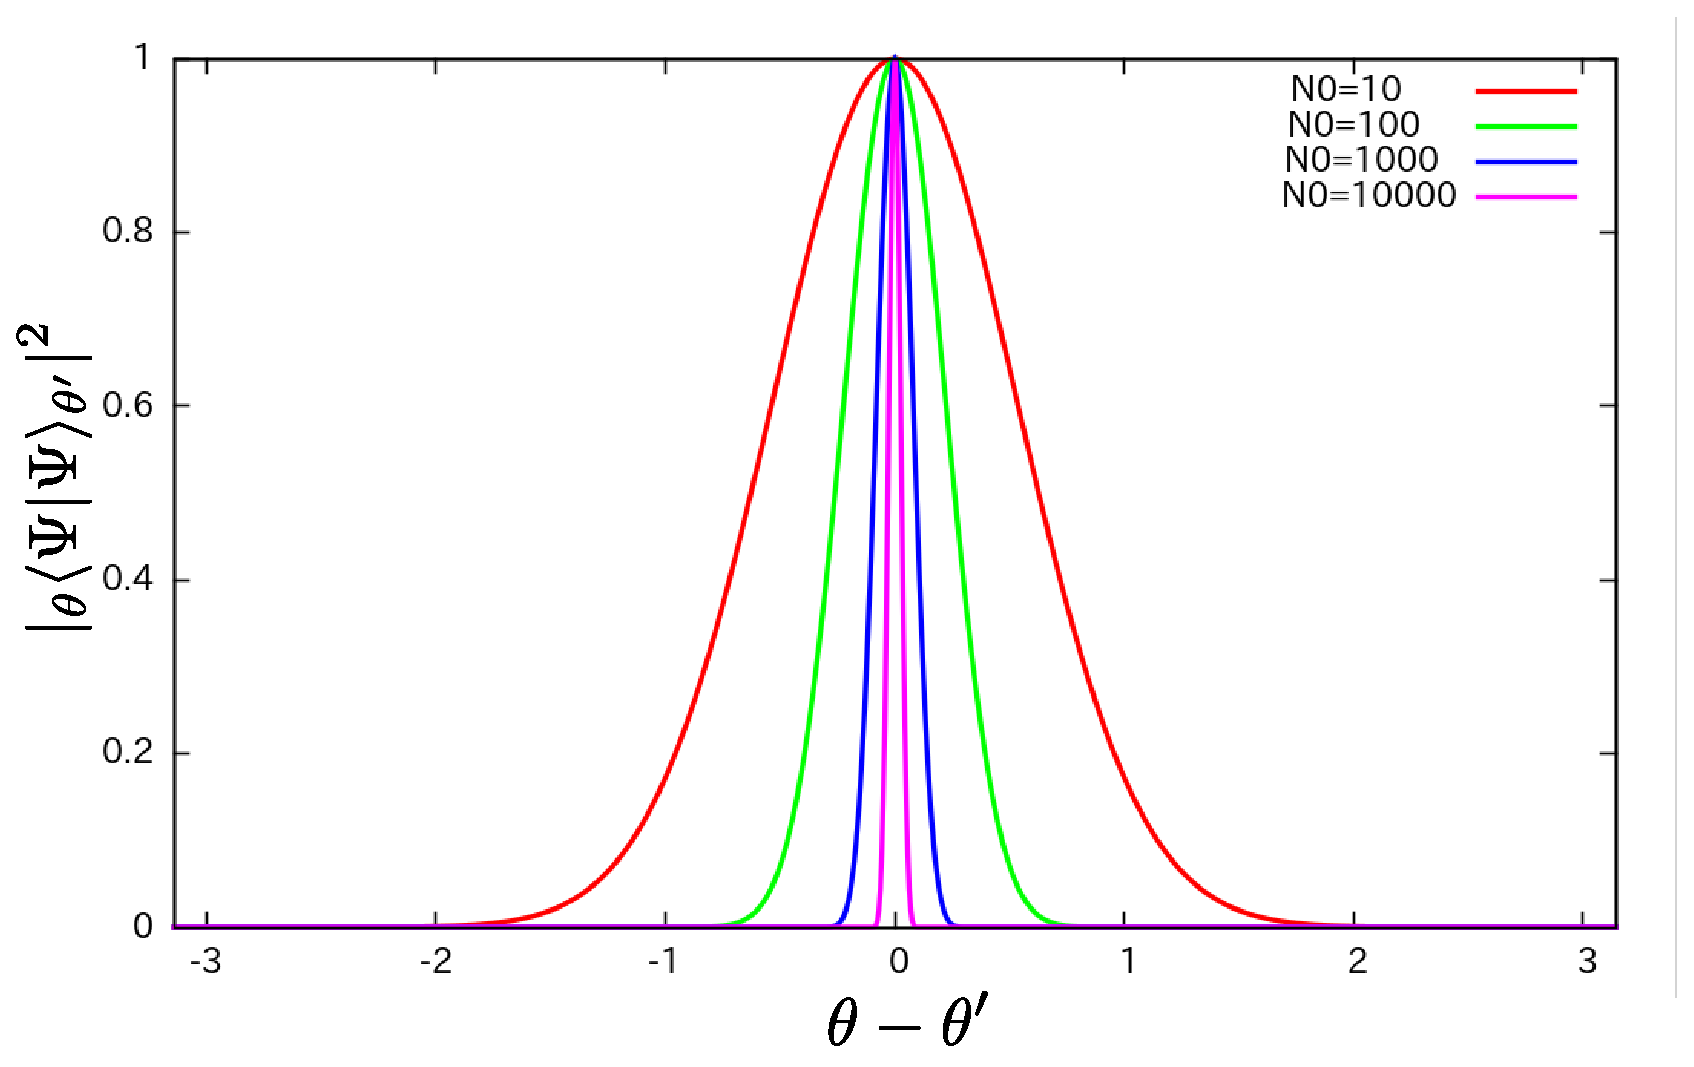
\includegraphics[width = 7cm]{./fig1.eps}
    \figcaption{$\kappa = \overline{n} = 1$}
    \label{fig1}
  \end{minipage}
  \begin{minipage}{0.5\hsize}
    \centering
    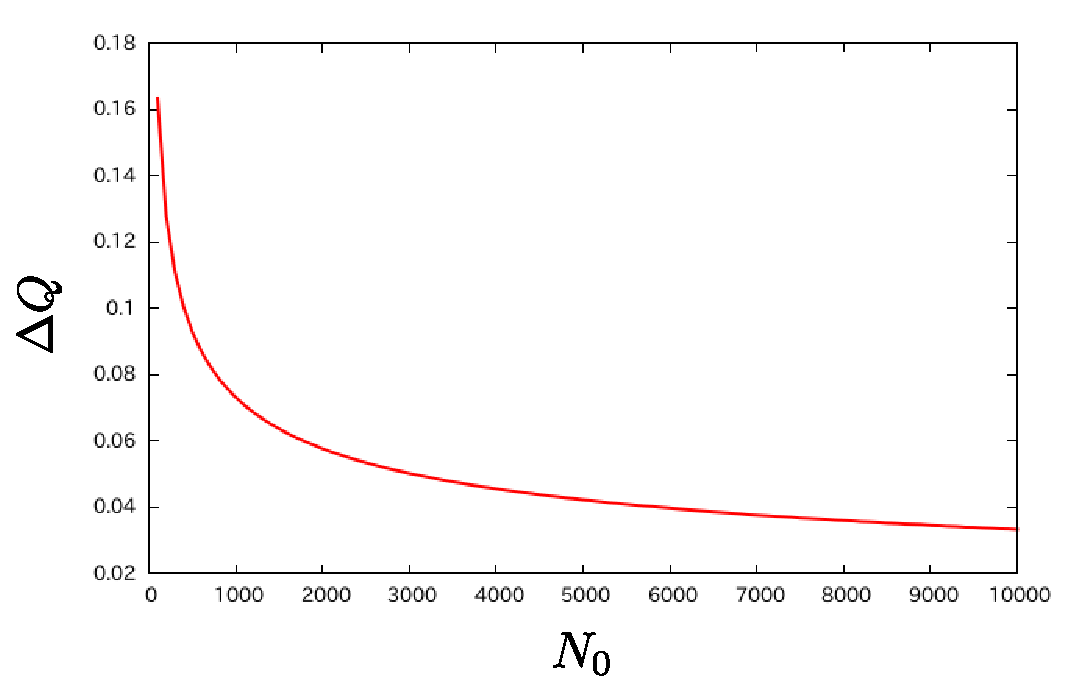
\includegraphics[width = 7cm]{./fig2.eps}
    \figcaption{$\kappa$が負の場合}
    \label{fig2}
  \end{minipage}
\end{figure}
$E(0)$の情報は$C_n$に組み込まれており, さらに$C_n$の関数列の形に制限は収束すること以外には特にない. $E(0)$は$C_n$の汎関数だとも言える. つまり, $C_n$の与え方によって熱浴を通じてエネルギーが流出するか流入するかが決まる\footnote{系の初期温度が熱浴の温度$T$より大きければ流出するし,逆なら流入するのが普通. 非平衡状態では温度は定義できないので, 正確には流入・流出を支配しているのは温度ではなくエントロピーである.}. 汎関数は無限個の自由度を持つ関数なので$E(0)$は単なる系のエネルギーの初期値だけでなく,熱浴との相関具合などの自由度を含んでいる(かもしれない). 図1にエネルギーが緩和する様子を示した.今回は$C_n = \frac{1}{n^2}, -\frac{1}{n^2} + \frac{5}{2n^5}$の2つを計算. これは単に流入と流出を見たかったために選んできたものであり, $C_n$が収束するような関数列を選べば緩和は観測できるはず.

また, $\kappa$が負の場合, 振幅は減衰することなく増幅することを図2で確認している.
\newpage
% ------------- 文章ここまで ---------------- %
\section{量子力学・統計力学の基礎知識}
\subsection{混合状態と密度行列}
熱が存在する場合, 一般に系は混合状態である.混合状態をやさしく説明すると...
\begin{screen}
  
  気体分子が100個と, その粒子の速度を測定する観測器がある系を考える. 仮に速度が$v_1$の分子が20個, $v_2$の分子が80個あったとする. その気体分子の速度の平均は, 速度$v_1$付近の粒子の状態を$\ket{\psi_1}$, $v_2$付近の粒子の状態を$\ket{\psi_2}$とすると,
  \begin{eqnarray*}
    \expval{\hat{v}} = \frac{1}{5}\bra{\psi_1}\hat{v}\ket{\psi_1} + \frac{4}{5}\bra{\psi_2}\hat{v}\ket{\psi_2}
  \end{eqnarray*}
  で与えられる.こういう形で期待値が与えられる場合, 系は混合状態であるという.ここで1/5と4/5は{\bf 統計由来の確率}であり, {\bf 量子力学的な確率}とは別物であることに注意. 前者が与えるのは粒子分布である. 古典粒子であればMaxwell-Boltzmann分布, 同種粒子であればFermi-Dirac分布とかBose-Einstein分布.その一方で, 後者が与えるのは量子論的な揺らぎである.揺らぎは$\Delta v_1$,$\Delta v_2$. $\bra{\psi}\hat{v}\ket{\psi}$は$v$の平均(期待値).
\end{screen}

つまり熱がある場合, 測定器で速度$v_1$の粒子が検出されるする確率は分布関数で与えられる. その粒子の速度を測定するとき, 期待される$v_1$という値からは少しずれて$v_1 + \Delta v_1$という値を取る. これが「値が確定しない」ということ.$\Delta v_1$の値は量子力学的な確率で与えられる.

期待値を得るもっと便利な表式を用意したい. ここで
\begin{eqnarray}
  \rho = \sum_np_n\ket{\psi_n}\bra{\psi_n}
\end{eqnarray}
を用意する. 上の例で言えば$p_11 = 1/5, p_2 = 4/5$である. これを密度行列と呼ぶ. 密度行列に求めたい物理量(今回は$\hat{v}$)を掛けてトレースを取る:
\begin{eqnarray}
  \nonumber    {\rm Tr}\rho\hat{v} &=& \sum_n\sum_m\bra{\Psi_m}p_n\ket{\psi_n}\bra{\psi_n}\hat{v}\ket{\Psi_m} = \sum_np_n\bra{\psi_n}\hat{v}\sum_m(\ket{\Psi_m}\bra{\Psi_m})\ket{\psi_n}\\
  &=&\sum_np_n\bra{\psi_n}\hat{v}\ket{\psi_n} = \expval{\hat{v}}
\end{eqnarray}
これは混合状態期待値である.ここで, c-数は交換可能, 完全系の性質$\sum_m\ket{\Psi_m}\bra{\Psi_m} = 1$である性質を用いている.またトレースの巡回対称性\footnote{証明してみよう!}(${\rm Tr}ABC = {\rm Tr}CAB = {\rm Tr}BCA$)より, $\hat{v}$を掛けるのは前からでも後ろからでもよい.

これで混合状態期待値を記述する統一的な表式が得られた. 密度行列に物理量を掛けてトレースを取ることで期待値が得られるということは, {\bf 密度行列は系の情報を全て持っている}ということになる. 系の情報を保持しているのはハミルトニアンであり, つまるところ密度行列を確定させるためにはハミルトニアンが必要である. 現に, 平衡状態における密度行列は$\rho = e^{-\beta H}$で与えられる\footnote{なぜこういう形で与えられるか考えてみよう!例えば$\expval{n} = {\rm Tr}a^\dagger a\rho$がBose-Einstein分布になることを確認すればいい}.

${\rm Tr}A\rho$は, 密度行列に含まれる情報のうち$A$以外の情報を切り捨てることを意味する. これをトレースアウトという.マスター方程式で密度演算子の時間発展を追えるが, Fullの密度演算子を計算するのは自由度が大きすぎて大変なので, 求めたい物理量以外をトレースアウトした形を用いるのが普通\footnote{山中研究室における普通です. 量子開放系の理論は完成していないので, 系統的にマスター方程式を作り, 解く方法はまだまとまっていない. 他の研究室では他の流儀があるかもしれない}.
\subsection{固有状態と不確定性}
初稿では$\hat{v}$(運動量$\hat{p}$でも同じこと)の固有状態として$\ket{\psi}$を定義したが, これはとてもよくない. 状態が$\hat{v}$の固有状態なら, 何度測定しても観測値は$v$になり量子的な揺らぎ$\Delta v$はなくなる. しかしながら不確定性原理は守られなければならないので, 運動量が確定する代わりに位置の不確定性が発散する. これは現実との対応を考えるとあまりにピーキーな設定である. 固有状態というのは量子力学の本質である揺らぎが存在しないとっても特別な状態です. 量子力学の固有状態でよく見かけるのは「エネルギー固有状態」ですが, これもエネルギーが確定する代わりにエネルギーと共役な物理量である時間の不確定性が発散します. ここでいう時間の不確定性とは「波動関数の時間的広がり」を表しています. エネルギー固有状態においては波動関数$\psi(x) e^{-iEt/\hbar}$の確率密度は変化しないので, 確率振幅の半値幅は無限大になります. これが$\Delta t = \infty$の意味です.
\subsection{ヒルベルト空間と平面波}
運動量の固有状態がマズいのは設定が現実的ではないということだけでなく, 量子力学の数学的構造にも反していることにあります. 量子力学における状態というものはヒルベルト空間($L^2$)で定義されるべきだが, 運動量の固有状態である平面波$e^{ipx}$は$L^2$をはみ出しており, 自乗可積分ではない\footnote{自乗可積分でないものを量子力学の枠組みに取り込むとBornの確率解釈が死にます}. つまり, 運動量の固有状態は量子力学では一般的に取り扱えないものなのである. しかし, 平面波というものは量子力学のいたるところで現れる. 例えば自由粒子の波動関数は平面波で記述されるし, 「平面波展開」というテクニックは様々なところで用いられる.

重要なのは境界条件である. 自由粒子は境界条件をなにも課していない\footnote{自由なのだから当然といえば当然}.Dirichlet境界条件を課すと状態は平面波ではなくなる. 一方で, 周期的境界条件が許される固体結晶では状態をBloch波で記述できる. 平面波で固体中の電子状態が記述できるということは, 固体中の電子は自由粒子とほぼ同等の状況下にあり, これが金属の電子伝導性を如実に説明している\footnote{古典的なDrudeモデルなどでは金属結晶の電子伝導性を説明しきれなかったようです}. また, $L^2$ではない平面波も, 適切な重み付けをして和, ないしは積分を取ると$L^2$になる場合がある.これがフーリエ級数展開とかフーリエ変換とか呼ばれているもの.

\subsection{第二量子化とFock空間}
第二量子化した量子力学は場の量子論とは異なる理論です\footnote{一般的に混同されがちですが, 山中研究室ではこれを断固として主張しています.}.なので, 第二量子化は場の理論ではなく多体量子力学の一形式と捉えられるべきです\footnote{もっとも異なることは, 「量子力学における状態はSchr\"odinger方程式で決定されるが, 場の理論における状態は理論を閉じるように選択されるもの」であること.粒子の生成・消滅で状態を記述する点は第二量子化された量子力学でも場の理論でも変わらない. ならば量子力学における真空(基底状態)は「粒子がひとつも存在しない状態」である. しかし, そのように真空を定義すると量子相転移を記述できなくなる. 例えば, Bose-Einstein凝縮(BEC)はひとつの相であり, 多数のBose粒子がエネルギー最低状態に落ち込み「真空」を形成しているものである. この「真空」には粒子が存在しているので量子力学では記述できない. 場の量子論ではBECが存在する状態を真空として定義することができる.}. 第二量子化された量子力学における最も気をつけなければいけない点は, 「生成消滅演算子で記述されるモードは原子の生成・消滅を記述しているわけではない」ということ. 生成消滅演算子は場の各点における励起を与えておりそれを素励起と呼ぶ. 素励起は波であり, 素励起の集まりが原子を記述している\footnote{原子にももちろん波動性がある}と考えてもいいかもしれない. 素励起のモードの固有状態(調和振動子における粒子数状態)のテンソル積で定義されるのがFock空間である. Fock空間はHilbert空間を無限自由度に拡張したものだと捉えて問題ない. つまり, 第二量子化では場の各点に調和振動子を設置し, それを無限個連結させたものであり, そのモードは素励起を表現するわけである.

今回の課題で与えられた生成消滅演算子がどのような粒子の生成消滅を記述しているのかはわからないが, 仮に第二量子化されたものを仮定するならば, そのモードは単純な粒子の追加とは違った意味合いを持つことは理解するべきでしょう\footnote{何言ってるかわからないかもしれません. 場の理論界隈の誤解されやすいかなり難しい話です.}.

\subsection{時間発展とユニタリー性}
量子マスター方程式による時間発展とHeisenberg方程式(Schr\"odinger方程式)による時間発展は何が違うのかというと, 緩和が記述できるかどうか. 量子力学におけるユニタリーな時間発展では系のノルムが保存しなければならないので,物理量の時間発展は振動し, 緩和することはない. Schr\"odinger方程式で物理量が減衰するようなグラフが得られたとしても, 時間領域を広げれば再び値が立ち上がる(revival)はずである. 仮にrevivalしないとしたら, それは時間発展のユニタリー性が壊れていることになる\footnote{一般解の一部を捨てることにより, 意図的にユニタリー性を壊すこともできる.}. 時間発展のユニタリー性を壊すのは番先生の本でもやってます\footnote{量子と非平衡系の物理―量子力学の基礎と量子情報・量子確率過程(2009)}. 一方, 開放系の統計力学では系・熱浴のハミルトニアンを分けて熱浴をトレースアウトするテクニックを用いてユニタリーな時間発展で緩和が記述できる.
\newpage
\chapter{場の量子論}
\section{Wickの定理}
摂動計算において重要な役割を果たす. ただし, この定理が成立するのは\textbf{生成消滅演算子の代数を満たすものに限られる. }つまり, ゼロモード演算子はWickの定理を満たさない. 
\subsection{概要}
ざっくり言うと
\begin{screen}
  場の演算子の時間順序積(T積)はそれらの演算子から構成される全ての可能な正規積(N積)と伝搬関数の積の和で表される.
\end{screen}
伝搬関数(因果Green関数, Feynman propagator)は
\begin{eqnarray}
  \Delta_F(\bm{x}_1-\bm{x}_2, t_1-t_2) = -i\bra{0}{\rm T}\left[\phi(\bm{x}_1, t_1)\phi^\dagger(\bm{x}_2, t_2)\right]\ket{0}
\end{eqnarray}
で与えられるので, $\phi$の可能な組を全て足し上げればよい. 伝搬関数は$\phi^\dagger, \phi$の組で作られるので, $\phi\phi, \phi^\dagger\phi^\dagger$の組は考えなくても良い. 
N積は生成演算子を前に, 消滅演算子を後ろに持ってくる順序積:
\begin{eqnarray}
  :\phi_1\phi^\dagger_2\phi_3\phi^\dagger_4:\ = \phi^\dagger_2\phi^\dagger_4\phi_1\phi_3
\end{eqnarray}

大事なことは, \textbf{N積の真空期待値は必ずゼロになるということ}と, \textbf{演算子が時間に依存していないならば勝手にT積をつけてもよい}ということ. 期待値を計算するための面倒な交換関係計算があるとき, Wickが使えることがある. 基本的には伝搬関数が真空で作られているので有限温度では使えないが, 議論を有限温度期待値に拡張したBlock-de Dominicsの定理というのがある. 有限温度系におけるWickの定理とかも呼ばれる. 
\subsection{具体例}
\subsubsection{n=2の場合}
\begin{eqnarray}
  {\rm T}[\phi_1\phi_2] =\ :\phi_1\phi_2: + \bra{0}{\rm T}[\phi_1\phi_2]\ket{0}
\end{eqnarray}
\subsubsection{n=3の場合}
\begin{eqnarray}
  {\rm T}[\phi_1\phi_2\phi_3] =\ :\phi_1\phi_2\phi_3: + \bra{0}{\rm T}[\phi_1\phi_2]\ket{0}\phi_3 + \bra{0}{\rm T}[\phi_1\phi_3]\ket{0}\phi_2 + \bra{0}{\rm T}[\phi_2\phi_3]\ket{0}\phi_1 
\end{eqnarray}
\subsection{証明}
\section{TFD形式による期待値計算}
$k$が連続自由度を持つ場合の期待値をTFDの力を借りて計算する.
\subsection{TFDのド基礎}
熱的真空は
\begin{eqnarray}
  \ket{0} &=& (1-f)\sum_mf^m\dket{m, m}\\
  \bra{0} &=& \sum_m\dbra{m, m}
\end{eqnarray}
で定義される. $f$はボルツマン因子. $f \neq e^{-\beta\omega}$のとき非平衡であるという. 熱的ブラ・ケットは双対ではない.
超演算子形式における$\dbra{I_R}\bullet\dket{\rho_R}$は熱的真空期待値$\ev{\bullet}{0}$に置き換えが可能\footnote{超演算子形式のチェック・チルダとTFDのノンチルダ・チルダは単射同型の関係にある. }. またBosonの熱的Bogoliubov変換の具体形は
\begin{eqnarray}
  b_{\bm{k}}^\dagger &=& \tilde{\xi_{\bm{k}}} + (1+n_{\bm{k}})\xi_{\bm{k}}^\dagger\\
  b_{\bm{k}} &=& \xi_{\bm{k}} + n_{\bm{k}}\tilde{\xi_{\bm{k}}}^\dagger
\end{eqnarray}
で与えられ, $\xi$演算子は熱的真空を消去する消滅演算子である:
\begin{eqnarray}
  \xi\ket{0} &=& \tilde{\xi}\ket{0} = 0\ ,\hspace{0.5cm} \bra{0}\xi^\dagger = \bra{0}\tilde{\xi}^\dagger = 0\\
  \comm{\xi}{\xi^\dagger} &=& \comm{\tilde{\xi_{\bm{k}}}}{\tilde{\xi_{\bm{k}'}}^\dagger} = \delta(\bm{k}-\bm{k}'), \hspace{0.5cm} \comm{\xi_{\bm{k}}}{\tilde{\xi_{\bm{k}'}}} = \comm{\xi_{\bm{k}}}{\tilde{\xi_{\bm{k}'}}^\dagger} = 0
\end{eqnarray}
この熱的真空, $\xi$演算子を用いて計算をする. 以下$x = (\bm{x}, t), y = (\bm{y}, s)$とする. 
\subsection{具体計算}
例として以下の計算をする:
\begin{eqnarray}
  \ev{R_3(x)R_3(y)} &\equiv& \bra{0}\frac{1}{(2\pi)^6}\int dk_1dk_2dk_3dk_4 b^\dagger_{k_1}b_{k_2}b^\dagger_{k_3}b_{k_4}e^{-i(k_1-k_2)x}e^{-i(k_3-k_4)y}e^{i(\omega_{k_1}-\omega_{k_2})t}e^{i(\omega_{k_3}-\omega_{k_4})s}\ket{0}\\
  \nonumber  &=& \frac{1}{(2\pi)^6}\int dk_1dk_2dk_3dk_4e^{-i(k_1-k_2)x}e^{-i(k_3-k_4)y}e^{i(\omega_{k_1}-\omega_{k_2})t}e^{i(\omega_{k_3}-\omega_{k_4})s}\\
  && \bra{0}\qty(\tilde{\xi_1} + (1+n_1)\xi_1^\dagger)\qty(\xi_2 + n_2\tilde{\xi_2}^\dagger)\qty(\tilde{\xi_3} + (1+n_3)\xi_3^\dagger)\qty(\xi_4 + n_4\tilde{\xi_4}^\dagger)\ket{0}
\end{eqnarray}
ここでは$\xi, n$の添字について$(k_1, k_2, k_3, k_4)\rightarrow(1, 2, 3, 4)$という置換をしている. 上式の熱的真空期待値を計算する:
\begin{eqnarray}
  &&\bra{0}\qty(\tilde{\xi_1} + (1+n_1)\xi_1^\dagger)\qty(\xi_2 + n_2\tilde{\xi_2}^\dagger)\qty(\tilde{\xi_3} + (1+n_3)\xi_3^\dagger)\qty(\xi_4 + n_4\tilde{\xi_4}^\dagger)\ket{0}\\
  =&&\bra{0}\tilde{\xi_1}\qty(\xi_2 + n_2\tilde{\xi_2}^\dagger)\qty(\tilde{\xi_3} + (1+n_3)\xi_3^\dagger)n_4\tilde{\xi_4}^\dagger\ket{0}\\
  =&&\bra{0}\qty(\tilde{\xi_1}\xi_2 + n_2\tilde{\xi_1}\tilde{\xi_2}^\dagger)\qty(n_4\tilde{\xi_3}\tilde{\xi_4}^\dagger + n_4(1+n_3)\xi_3^\dagger \tilde{\xi_4}^\dagger)\ket{0}\\
  =&&\bra{0}\qty(\tilde{\xi_1}\xi_2 + n_2\Bqty{\tilde{\xi_2}^\dagger\tilde{\xi_1} + \comm{\tilde{\xi_1}}{\tilde{\xi_2}^\dagger}})\qty(n_4\Bqty{\tilde{\xi_4}^\dagger\tilde{\xi_3} + \comm{\tilde{\xi_3}}{\tilde{\xi_4}^\dagger}} + n_4(1+n_3)\xi_3^\dagger \tilde{\xi_4}^\dagger)\ket{0}\\
  =&&\bra{0}\qty(\tilde{\xi_1}\xi_2 + n_2\delta(1-2))\qty(n_4\delta(3-4) + n_4(1+n_3)\xi_3^\dagger \tilde{\xi_4}^\dagger)\ket{0}\\
  \nonumber  = &&\bra{0}\qty(\tilde{\xi_1}\xi_2n_4\delta(3-4) + \tilde{\xi_1}\xi_2\xi_3^\dagger \tilde{\xi_4}^\dagger n_4(1+n_3) + n_2n_4\delta(1-2)\delta(3-4) + \xi_3^\dagger \tilde{\xi_4}^\dagger n_2n_4(1+n_3)\delta(1-2))\ket{0}\\
  \\
  = &&\bra{0}\qty(\tilde{\xi_1}\xi_2\xi_3^\dagger \tilde{\xi_4}^\dagger n_4(1+n_3) + n_2n_4\delta(1-2)\delta(3-4))\ket{0}\\
  = &&\bra{0}\Bqty{n_4(1+n_3)\delta(1-4)\delta(2-3) + n_2n_4\delta(1-2)\delta(3-4)}\ket{0}
\end{eqnarray}
よって
\begin{eqnarray}
  \nonumber  \ev{R_3(x)R_3(y)} &\equiv&\qty(\frac{1}{(2\pi)^3}\int dk n_k)^2 + \frac{1}{(2\pi)^6}\int dk_1dk_2 e^{-i(k_1-k_2)(x-y)}e^{i(\omega_{k_1}-\omega_{k_2})(t-s)}n_1(1+n_2)\label{expectation2}\\
\end{eqnarray}
\subsection{Block-de Dominicsの定理}
TFD形式だと計算が簡単になることがわかった\footnote{超演算子形式のままだとトレース演算になるのでなかなか面倒. }. ただ, 熱平均についてはBlock-de Dominicsの定理というWickの定理に対応するものがあるので, もっと簡単に計算できそうである. $b_1\sim b_6$まであるものを考えるが, $x, y$がcoupleするか否かは区別しないといけない\footnote{たとえば$1x-2x$がcoupleすると対応するデルタ関数$\delta(1-2)$が出てきて$e^{-i(k_1 - k_2)(x-y)}, e^{i(\omega_1 - \omega_2)(t-s)}$が消える.これは(\ref{expectation2})の右辺第一項にあたる項の起源. 一方で$x-y$のcross couplingがあるとexponentialの空間・時間成分が消えずに残る. これが(\ref{expectation2})の右辺第二項にあたる.}:
\begin{eqnarray}
  \ev{R_1(x)R_1^\dagger(y)} &\sim& \bra{0}b_{1x}^\dagger b^\dagger_{2x} b_{3x} b^\dagger_{4y} b_{5y} b_{6y} \ket{0} =\bra{0}{\rm T} \bqty{b_{1x}^\dagger b^\dagger_{2x} b_{3x} b^\dagger_{4y} b_{5y} b_{6y} }\ket{0}\\
  &=& 2\bra{0}{\rm T}\wick{321}{<1b_{1x}^\dagger <2b^\dagger_{2x} <3b_{3x} >3b^\dagger_{4y} >1b_{5y} >2b_{6y} }\ket{0} + 4\bra{0}{\rm T}\wick{321}{<1b_{1x}^\dagger <2b^\dagger_{2x} >1b_{3x} <3b^\dagger_{4y} >2b_{5y} >3b_{6y} }\ket{0}\\
  &=&2\ev{b^\dagger_{1x}b_{5y}}\ev{b^\dagger_{2x}b_{6y}}\ev{b_{3x}b^\dagger_{4y}} + 4\ev{b^\dagger_{1x}b_{3x}}\ev{b^\dagger_{2x}b_{5y}}\ev{b^\dagger_{4y}b_{6y}}\\
  \nonumber  &=& 2\delta(1-5)\delta(2-6)\delta(3-4)n_1n_2(1+n_3) + 4\delta(1-3)\delta(2-5)\delta(4-6)n_1n_2n_4\\
\end{eqnarray}
$\xi$演算子で真面目に計算しなくてもいける. 
\section{Gell-Mann-Lowの定理}
\subsection{断熱因子}
ハミルトニアンの摂動部が断熱因子を持っている場合を考える:
\begin{eqnarray}
  H = H_0 + e^{-\epsilon|t|}H_I
\end{eqnarray}
これは$t = 0$でfullの相互作用を取り入れた系になり, $t \rightarrow \pm\infty$で自由粒子になるようなハミルトニアンである. ここで, $t = t_0$かつ$t_0 \sim -\infty$で相互作用描像の状態が非摂動ハミルトニアンの固有状態になっている場合を考える\footnote{相互作用描像も自由粒子のハイゼンベルグ描像と一致するという近似できる. }:
\begin{eqnarray}
  H_0\ket{\Psi(t_0)}_I = E_0\ket{\Psi(t_0)}_I
\end{eqnarray}
さらに$t_0 \sim -\infty$であることから時間発展演算子を用いてハイゼンベルグ描像は
\begin{eqnarray}
  \ket{\Psi}_{\rm H} =  \ket{\Psi(0)}_I = U_\epsilon(0, t_0)\ket{\Psi(t_0)}_I= U_\epsilon(0, -\infty)\ket{\Psi(t_0)}_I\label{5eq1}
\end{eqnarray}
と書ける. これは, 相互作用系の状態が非摂動系の固有状態を用いて表現できたことを意味している.

あとは$\epsilon$について考える必要がある. そもそもこの系は2つの粒子の散乱実験をテーマにしたようなものである. 2つの粒子が$t = 0$で衝突することを考えるとき, 相互作用が効いてくるのは$t = 0$近傍のみであって, それ以外は自由粒子とほぼ同じ振る舞いをするだろうというアイデアから断熱因子は導入されている. 粒子を平面波的に記述するためにも$\epsilon\rightarrow 0$としたいが, この極限のもとで果たして(\ref{5eq1})は意味ある結果を与えるのだろうか?

これに答えるのがGell-Mann-Lowの定理である.\textbf{以降は基底状態に対する議論であることに注意.}
\subsection{概要}
Gell-Mann-Lowの定理が主張することは
\begin{eqnarray}
  \lim_{\epsilon\rightarrow0}\frac{U_\epsilon(0, -\infty)\ket{\phi_0(-\infty)}_I}{_I\bra{\phi_0(-\infty)}U_\epsilon(0, -\infty)\ket{\phi_0(-\infty)}_I} = \frac{\ket{\Psi_0}_H}{_I\expval{\phi_0(-\infty)|\Psi_0}_H}\label{gml}
\end{eqnarray}
が存在するなら固有状態$\ket{\Psi_0}_{\rm H}$はwell-definedであり, 固有値は
\begin{eqnarray}
  E-E_0 = \frac{_I\bra{\phi_0(-\infty)}H_I\ket{\Psi_0}_H}{_I\expval{\phi_0(-\infty)|\Psi_0}_H}
\end{eqnarray}
で与えられるということである. ここで添字の0は真空を意味している. また, $\ket{\phi_0(-\infty)}$は非摂動ハミルトニアンの固有状態になっているので解析的に求めることができる. あとは, (\ref{gml})が成立するかどうかが問題になる.
\subsection{証明}

\section{Tips}
忘れやすいことをメモしておきます.
\subsection{Heisenberg描像}
Schr\"odinger描像は時間発展の情報が状態にある:
\begin{eqnarray}
  i\hbar\partial_t\ket{\psi(t)} &=& \hat{H}\ket{\psi(t)}\\
  \expval{\hat{A}} &=&\ _S\!\bra{\psi(t)}\hat{A}\ket{\psi(t)}_S
\end{eqnarray}
Schr\"odinger方程式の形式解
\begin{eqnarray}
  \ket{\psi(t)} = e^{-i\hat{H}t/\hbar}\ket{\psi(0)}
\end{eqnarray}
を用いると期待値は
\begin{eqnarray}
  \expval{\hat{A}} &=&\ _S\!\bra{\psi(0)}e^{i\hat{H}t/\hbar}\hat{A}e^{-i\hat{H}t/\hbar}\ket{\psi(0)}_S
\end{eqnarray}
と書くことができる. Heisenberg描像における演算子と状態は
\begin{eqnarray}
  \hat{A}_{\rm H}(t) &=& e^{i\hat{H}t/\hbar}\hat{A}e^{-i\hat{H}t/\hbar}\\
  \ket{\psi}_{\rm H} &=&  \ket{\psi(0)}_{\rm S}
\end{eqnarray}
\subsection{相互作用描像}
ハミルトニアンを
\begin{eqnarray}
  H = H_0 + H_I
\end{eqnarray}
のように非摂動部$H_0$と摂動部$H_I$に分割する. 分割の方法は任意だが, 非摂動部を解析的に解ける形にしておくのが普通\footnote{たとえば生成消滅演算子の2次で記述できればBogoliubov変換を通して対角化が可能. IZMFにおいては真空を$\ket{0}_{\rm ex}\ket{\Psi_0}$のように励起部とゼロモード部の直積にする. ゼロモードの真空は非摂動部にゼロモードの高次を取り込んで場の分割条件を守るようにカウンター項を決定する. ゼロモードは生成消滅演算子の代数を持っていないので取り扱いは励起部とは本質的に異なることに注意. }. Heisenberg描像の時と同じように形式解を代入する:
\begin{eqnarray}
  \ket{\psi(t)}_{\rm S} = e^{-i(\hat{H_0} + \hat{H_I})t/\hbar}\ket{\psi(0)}_{\rm S}
\end{eqnarray}
ここで, 相互作用描像の状態を
\begin{eqnarray}
  \ket{\psi(t)}_{\rm I} \equiv e^{i\hat{H_0}t/\hbar}\ket{\psi(t)}_{\rm S} &=& e^{-i\hat{H_I}t/\hbar}\ket{\psi(0)}_{\rm S}\\
  &=& e^{-i\hat{H_I}t/\hbar}\ket{\psi}_{\rm H}
\end{eqnarray}
と定義する. つまり, \textbf{相互作用描像の状態は摂動部$H_{\rm I}$(相互作用ハミルトニアン)による時間変化を担っている. }一方で相互作用描像の演算子は
\begin{eqnarray}
  A_{\rm I}(t) \equiv e^{i\hat{H_0}t/\hbar}\hat{A}_{\rm S}e^{-i\hat{H_0}t/\hbar}
\end{eqnarray}
で定義され, \textbf{非摂動部$H_0$による時間変化を担っている. }

この描像においては$t = 0$で真空はHeisenberg描像と一致し, 演算子の時間発展はHeisenberg方程式
\begin{eqnarray}
  i\hbar\partial_tA_{\rm I}(t) = [A_{\rm I}(t), H_0]
\end{eqnarray}
で記述される. ここで重要なのが, \textbf{演算子の時間発展は非摂動ハミルトニアンで記述されている}ということ. 演算子の時間発展を追うのは難しくなさそう\footnote{もちろん非摂動ハミルトニアンが解析的に解ける形である場合に限る}. 一方で状態の時間発展は
\begin{eqnarray}
  i\hbar\partial_t\ket{\psi(t)}_I = H_{\rm I}\ket{\psi(t)}_I
\end{eqnarray}
のように, 解析的に解けない相互作用ハミルトニアンで記述されているのでそんなに簡単ではない. よって, 状態は摂動展開によって評価することになる.
\subsection{デルタ関数のFourier変換表示}
1次元Fourier変換
\begin{eqnarray}
  f(x) &=& \frac{1}{\sqrt{2\pi}}\int dk \tilde{f}(k)e^{ikx}\\
  \tilde{f}(k) &=& \frac{1}{\sqrt{2\pi}}\int dx f(x)e^{-ikx}
\end{eqnarray}
を相互に代入する:
\begin{eqnarray}
  f(x) &=& \frac{1}{\sqrt{2\pi}}\int dk \left(\frac{1}{\sqrt{2\pi}}\int dx' f(x')e^{-ikx'}\right)e^{ikx}\\
  &=& \int dx' \left(\frac{1}{2\pi}\int dk e^{ik(x-x')}\right)f(x')
\end{eqnarray}
これより
\begin{eqnarray}
  \delta(x-x') &=& \frac{1}{2\pi}\int dk e^{ik(x-x')}\\
\end{eqnarray}
ひいては
\begin{eqnarray}
  \delta(x) &=& \frac{1}{2\pi}\int dk e^{ikx} = \frac{1}{2\pi}\int dk e^{-ikx}
\end{eqnarray}
であることがわかる. 「1のFourier変換は$2\pi\delta(x)$だ」という表現もできる. 
\subsection{$\bm{k}$が離散・連続の場合の$\expval{a_{\bm k}^\dagger a_{\bm{k}'}}$}
\subsubsection{有限体積の場合}
まずは$\left[\psi(x), \psi^\dagger(x')\right] = \delta(x - x')$を満たす一般的な演算子$\psi(x)$を離散変数$k_n$で展開した場合を考える. 体積$L$の一次元系について:
\begin{eqnarray}
  \psi(x) = \frac{1}{\sqrt{L}}\sum_{n=-\infty}^{n=\infty}e^{ik_nx}a_{k_n}
\end{eqnarray}
ただし$k_n = \frac{2\pi}{L}n$とする. すると,
\begin{eqnarray}
  \int dx\ \psi(x)e^{-ik_nx} &=& \frac{1}{\sqrt{L}}\sum_{n'}\int dx\ e^{-i(k_n-k_{n'})x}a_{k_{n'}}\\
  &=& \frac{1}{\sqrt{L}}\sum_{n'}L\delta_{nn'}a_{k_{n'}} = \sqrt{L}a_{k_n}\\
  \therefore a_{k_n} &=& \frac{1}{\sqrt{L}}\int dx\ \psi(x)e^{-ik_nx}  
\end{eqnarray}
このとき交換関係は
\begin{eqnarray}
  [a_{k_n}, a^\dagger_{k_{n'}}] = \frac{1}{L}\int dx dx'\ e^{-i(k_nx - k_{n'}x')}\left[\psi(x), \psi^\dagger(x')\right] = \frac{1}{L}\int dx \ e^{-i(k_n - k_{n'})x} = \delta_{nn'}
\end{eqnarray}
であり, 確かに本文の記述の通り,
\begin{eqnarray}
  \expval{a_{k_n}^\dagger a_{k_n}} = \frac{1}{e^{\beta\omega_{k_n}}-1} \equiv n_{k_n}
\end{eqnarray}
である.
\subsubsection{熱力学極限}
$L\rightarrow\infty$, つまり$k$の連続極限を取ることを考える. Fourier変換から
\begin{eqnarray}
  \psi(x) = \frac{1}{\sqrt{2\pi}}\int dk\ e^{ikx}a_k
\end{eqnarray}
となって欲しい. 交換関係が$[a_k, a_{k'}^\dagger] = \delta(k - k')$に変わる. これを守るために, $a_{k_n}\rightarrow ca_k$となる$c$を求める. $\sum_n\Delta ke^{ik_nx}\rightarrow\int dk e^{ikx}$かつ$\Delta k = \frac{2\pi}{L}$であることを用いて
\begin{eqnarray}
  \psi(x) = \frac{1}{\sqrt{L}}\sum_{n=-\infty}^{n=\infty}\frac{2\pi}{L}e^{ik_nx}a_{k_n}\frac{L}{2\pi}\rightarrow \frac{\sqrt{L}}{2\pi}\int dk e^{ikx} ca_n
\end{eqnarray}
となる. これより
\begin{eqnarray}
  c = \sqrt{\frac{2\pi}{L}}
\end{eqnarray}
以上より,
\begin{eqnarray}
  \expval{a_k^\dagger a_k} = \frac{L}{2\pi}n_k\label{particle}
\end{eqnarray}
であることがわかる. 今回は体積無限の系を考えているので,
\begin{eqnarray}
  \int_{-\infty}^\infty dx = L
\end{eqnarray}
であることから,
\begin{eqnarray}
  \delta(x) &=& \frac{1}{2\pi}\int dk\  e^{ikx}\\
  \Longrightarrow \delta(0) &=& \frac{1}{2\pi}\int dk = \frac{L}{2\pi}
\end{eqnarray}
つまり式(\ref{particle})はデルタ関数を用いて
\begin{eqnarray}
  \expval{a_k^\dagger a_k} = \delta(0)n_k\label{particle}
\end{eqnarray}
と表現できる.
\subsection{デルタ関数が体積になること}
\begin{eqnarray}
  \int^\infty_{-\infty} d\bm{x} = V
\end{eqnarray}
であり, デルタ関数のFourier変換表示
\begin{eqnarray}
  \delta(x) = \frac{1}{(2\pi)^3}\int dk e^{ikx}\hspace{0.5cm}\Longrightarrow \hspace{0.5cm}\delta(0) = \frac{1}{(2\pi)^3}\int dx = \frac{V}{(2\pi)^3}
\end{eqnarray}
\subsection{ハミルトニアンの対角化とBogoliubov-de Gennes方程式}
\subsubsection{対角化とは}
ハミルトニアンの対角化とはハミルトニアンを生成消滅演算子を用いて
\begin{eqnarray}
  H = \sum_\ell \omega_{\ell} a_\ell a_\ell^\dagger\label{diagonal}
\end{eqnarray}
と表現することである. $\omega_\ell>0$であれば$a_\ell$が消去する$\ket{0}$が$H$の基底状態であることは量子力学における調和振動子の議論から明らか. $\omega_\ell < 0$である場合は$a_\ell$でいくらでもエネルギーを下げることができるので, $a_\ell$が張るFock空間には基底状態が存在しない\footnote{こういうのをLandau不安定性という. }.

正準交換関係を満たす場の演算子から生成消滅演算子を構成するのは簡単. 正規直交完全系$w_\ell$で場の演算子$\varphi$を展開する:
\begin{eqnarray}
  \varphi = \sum_\ell a_\ell(t)w_\ell(\bm{x}), \hspace{0.5cm} a_\ell = \int d\bm{x} \omega_\ell(\bm{x})\varphi(x)\label{expansion}
\end{eqnarray}
ただし
\begin{eqnarray}
  \sum_\ell w_\ell(\bm{x}) w^*_\ell(\bm{x}') = \delta(\bm{x}-\bm{x}'),\hspace{0.5cm}  \int d\bm{x} w_\ell(\bm{x}) w^*_{\ell'}(\bm{x}) = \delta_{\ell\ell'}
\end{eqnarray}
である. 
$\comm{\varphi(x)}{\varphi^\dagger(x')} = \delta(x - x')$から
\begin{eqnarray}
  \comm{a_\ell}{a^\dagger_{\ell'}} = \delta_{\ell\ell'}
\end{eqnarray}
であることがわかり, この$a, a^\dagger$は生成消滅演算子の代数を満たしている. つまり, 対角化のためには(\ref{diagonal})となるような適切な$w_\ell$を見つければ良い. $w_\ell$が変わると$a_\ell$の定義も変わるので, (\ref{expansion})で展開した時$a_\ell$が生成消滅演算子になるように構成しなければいけない. 

ここであるハミルトニアン
\begin{eqnarray}
  H_0 = \int d\bm{x} \varphi^\dagger(x)h_0(\bm{x})\varphi(x)\label{unperturb}
\end{eqnarray}
を対角化したい. $h_0$の固有値方程式
\begin{eqnarray}
  h_0(\bm{x})w_\ell(\bm{x}) = \omega_\ell w_\ell(\bm{x})
\end{eqnarray}
から正規直交完全系をつくり, それでもって$\varphi$を展開する:
\begin{eqnarray}
  H_0 &=& \int d\bm{x} \sum_{\ell\ell'}a^\dagger_\ell(t)w^*_\ell(\bm{x})h_0(\bm{x})w_{\ell'}(\bm{x})a_{\ell'}(t)\\
  &=& \int d\bm{x} \sum_{\ell\ell'}a^\dagger_\ell(t)w^*_\ell(\bm{x})\omega_{\ell'}w_{\ell'}(\bm{x})a_{\ell'}(t)\\
  &=& \sum_{\ell\ell'}\omega_{\ell'}a^\dagger_\ell(t)a_{\ell'}(t)\delta_{\ell\ell'}\\
  &=& \sum_{\ell}\omega_{\ell}a^\dagger_\ell(t)a_{\ell}(t)
\end{eqnarray}
対角化完了. つまり, (\ref{unperturb})のようなハミルトニアンは$h_0$の固有値問題を解き, その固有完全系でもって場の演算子を展開することで対角化ができる. これがほぼ唯一の対角化の方法である.
\subsubsection{Bogoliubov-de Gennes方程式}
冷却原子系のハミルトニアンの非摂動部をdoubletで書くと
\begin{eqnarray}
  H_u &=&  \int d\bm{x}
  \begin{pmatrix}
    \varphi^\dagger&-\varphi 
  \end{pmatrix}
  \begin{pmatrix}
    \calL &\calM\\
    -\calM^* &-\calL
  \end{pmatrix}
  \begin{pmatrix}
    \varphi\\
    \varphi^\dagger 
  \end{pmatrix}\\
  &=& \int d\bm{x} \overline{\Phi}T\Phi
\end{eqnarray}
となる\footnote{マイナスをつけたのはdoubletの$\Phi, \overline{\Phi}$が正準交換関係を満たすようにするため}. 先ほどのアナロジーから, $T$についての固有値方程式を解き, その固有関数系で$\Phi$を展開すれば非摂動部の対角化が可能である. この$T$についての固有値方程式がBogoliubov-de Gennes方程式である. $T$が一般にエルミートでないことに注意.
\subsection{一様系のBogoliubov-de Gennes方程式}
一様系ではBogoliubov変換とBogoliubov-de Gennes方程式による対角化は等価であり,解析的に計算が可能. 場の演算子をFourier変換:
\begin{eqnarray}
  \varphi = \frac{1}{\sqrt{(2\pi)^3}}\int d\bm{k} b_{\bm k}e^{i\bm{kx}}
\end{eqnarray}
ここで場を
\begin{eqnarray}
  \psi = \xi + \varphi
\end{eqnarray}
のように分割している. これを用いると冷却原子系の非摂動ハミルトニアンは
\begin{eqnarray}
  H_2 &=& \int d\bm{k}
  \begin{pmatrix}
    b_{\bm k}^\dagger &-b_{\bm -k} 
  \end{pmatrix}
  \begin{pmatrix}
    \calL_k &\calM\\
    -\calM^* &-\calL_k
  \end{pmatrix}
  \begin{pmatrix}
    b_{\bm k}\\
    b_{\bm -k}^\dagger 
  \end{pmatrix}
\end{eqnarray}
ただし
\begin{eqnarray}
  \calL_k &=& \varepsilon_k + gn_0,\ \calM = gn_0e^{2i\theta}\\
  \varepsilon_k &=& \frac{\hbar^2k^2}{2m},\ \xi(\bm{x}) = \sqrt{n_0}e^{i\theta},\ \mu = gn_0
\end{eqnarray}
つまり, k表示されたBdG行列の固有値問題を解けばよいことになり, さらに$\calL_k, \calM$は演算子を含まないので簡単である. これを解くと
\begin{eqnarray}
  \omega_k = \sqrt{\varepsilon_k(\varepsilon_k + 2gn_0)}
\end{eqnarray}
を得る.
\newpage
\chapter{研究 - 3次元一様有限温度系のゼロモード}
2015年度夏の学校. 有限温度ゼロモード系における自己無撞着計算がメイン. 有限温度系で重要な計算や考え方が頻出.

また, 夏の学校時点では凝縮粒子数の定義にゼロモード演算子の期待値を加えていなかったため, Depletionは相互作用定数$g$が小さいところで持ち上がる結果を得た. 凝縮粒子数の定義を変えたところ, Depletionは相互作用定数$g$に対してロバストになった. こっちのほうが自然だろうというのが今のところの結論. 
\section{問題設定}
粒子間の相互作用を考慮に入れてゼロモード演算子の期待値を計算をする.この効果のことを量子補正と呼ぶ.\\
相互作用がある場合はゼロ温度でも全ての粒子が凝縮するわけではないことから,今回は主に凝縮粒子数と非凝縮粒子数の割合(depletion)が相互作用によってどのように変わるか,またゼロモードの寄与がある場合とない場合で結果がどのように変わるかを見る.

まずは,量子補正を考慮した方程式の定式化から入る.
\subsection{冷却原子気体系のハミルトニアン}
冷却原子気体のハミルトニアンは以下のように与えられる.
\begin{eqnarray}
  H_{\rm H}=\int d\bm{x}\left[\psi_{\rm H}^\dagger(h_0-\mu)\psi_{\rm H} +\frac{g}{2}\psi_{\rm H}^\dagger\psi_{\rm H}^\dagger\psi_{\rm H}\psi_{\rm H}\right]
\end{eqnarray}
添字のHはHeisenberg描像であることを示している.$\mu$は化学ポテンシャル,$g$は相互作用定数,$h_0$は
\begin{eqnarray}
  h_0 = -\frac{\nabla^2}{2m}
\end{eqnarray}
であるような一様系を取り扱う.場の演算子$\psi_{\rm H}$は同時刻交換関係
\begin{eqnarray}
  &&\left[\psi_{\rm H}(\bm{x},t),\psi_{\rm H}^\dagger(\bm{x}',t) \right] = \delta(\bm{x} - \bm{x}')\\
  &&\left[\psi_{\rm H}(\bm{x},t),\psi_{\rm H}(\bm{x}',t) \right] = 0,\ \ \ \ \ \left[\psi_{\rm H}^\dagger(\bm{x},t),\psi_{\rm H}^\dagger(\bm{x}',t) \right] = 0
\end{eqnarray}
を満たす.このとき,$\psi_{\rm H}$は真空期待値を持つ:
\begin{eqnarray}
  \langle 0|\psi_{\rm H}(\bm{x})|0\rangle = \xi(\bm{x})\label{vaccum_ex1}
\end{eqnarray}
$\xi$は秩序変数と呼ばれ,$|\xi|^2$は凝縮体の密度と解釈できる.秩序変数は今回は時間に依存しないと仮定する.
場の演算子を以下のように分割する:
\begin{eqnarray}
  \psi_{\rm H} = \xi + \varphi_{\rm H}
\end{eqnarray}
$\xi$は凝縮体を記述する古典場,$\varphi_{\rm H}$は非凝縮体を記述する場の演算子と解釈できる.これは同時刻交換関係
\begin{eqnarray}
  \left[\varphi_{\rm H}(\bm{x},t),\varphi^\dagger_{\rm H}(\bm{x}',t)\right]  = \delta(\bm{x}-\bm{x}')\label{equal_time_commutation}
\end{eqnarray}
を満たしている.

ハミルトニアンを$\varphi_{\rm H}$の次数について整理すると
\begin{eqnarray}
  &&H_{{\rm H},1} = \int d\bm{x}\left[\varphi^\dagger_{\rm H}(h_0 - \mu + g|\xi|^2)\xi + \varphi_{\rm H}(h_0 - \mu + g|\xi|^2)\xi^*\right]\\
  &&H_{{\rm H},2} = \int d\bm{x}\left[\varphi^\dagger_{\rm H} {\cal L}\varphi_{\rm H} + \frac{1}{2}\varphi_{\rm H}{\cal M^*}\varphi_{\rm H}+\frac{1}{2}\varphi^\dagger_{\rm H}{\cal M}\varphi^\dagger_{\rm H}\right]\\
  &&H_{{\rm H},3} = g\int d\bm{x}\left[\xi^*\varphi^\dagger_{\rm H}\varphi_{\rm H}\varphi_{\rm H} + \xi\varphi^\dagger_{\rm H}\varphi^\dagger_{\rm H}\varphi_{\rm H} \right] \\
  &&H_{{\rm H},4} = \frac{g}{2}\int d\bm{x}\ \varphi^\dagger_{\rm H}\varphi^\dagger_{\rm H}\varphi_{\rm H}\varphi_{\rm H}
\end{eqnarray}
であり
\begin{eqnarray}
  {\cal L} = h_0 - \mu +2g|\xi|^2,\ \ \ \ \ {\cal M}=g\xi^2
\end{eqnarray}
である.

\subsection{相互作用描像}
系が十分低温であり相互作用$g$が小さいとする.この場合$H_{{\rm H},3},H_{{\rm H},4}$の効果は小さいとして,非摂動ハミルトニアンを$H_{{\rm H},u}=H_{{\rm H},1}+H_{{\rm H},2}$のように選び,Heisenberg描像から相互作用描像に移行する.まず
\begin{eqnarray}
  i\frac{d}{dt}U(t,t_0)=U(t,t_0)H_{{\rm H},p},\ \ \ \ \ U(t_0,t_0)=1,\ \ \ \ \ H_{{\rm H},p} = H_{\rm H} - H_{{\rm H},u}
\end{eqnarray}
を満たすようなユニタリー演算子$U(t,t_0)$を考え,Heisenberg描像の任意の演算子$A_{\rm H}(t)$を用いて相互作用描像の演算子を
\begin{eqnarray}
  A(t) = U(t,t_0)A_{\rm H}(t)U^{-1}(t,t_0)
\end{eqnarray}
と定義する.$t_0$はHeisenberg描像と相互作用描像が一致する時間である.Heisenberg方程式は
\begin{eqnarray}
  i\frac{d}{dt}A(t) = \left[A(t),H_u(t)\right]
\end{eqnarray}
である.ここで$A=H_u$と代入すると時間に依存しないことがわかるので,$H_u = H_{{\rm H},u}$である.

$U(t,t_0)$の時間発展は$H_{{\rm H},p}=H_{{\rm H},3}+H_{{\rm H},4}$に依存し,かつその効果が小さいことから場の演算子の摂動ゼロ次は
\begin{eqnarray}
  \langle0|\varphi_{\rm H}(x)|0\rangle = \langle0| U^{-1}(t,t_0)\varphi(x)U(t,t_0)|0\rangle \simeq \langle0|\varphi(x)|0\rangle
\end{eqnarray}
となっている.また相互作用描像のHeisenberg方程式より
\begin{eqnarray}
  i\frac{\partial}{\partial t}\varphi(x) = \left[\varphi(x),H_u\right]\label{Heisenberg}
\end{eqnarray}
であることがわかる.これ以降$x=(\bm{x},t)$とする.つまり,場の分割条件を
\begin{eqnarray}
  \langle0|\varphi_{\rm H}(x)|0\rangle \simeq \langle0|\varphi(x)|0\rangle = 0
\end{eqnarray}
とした場合,この性質が保存するためには式(\ref{Heisenberg})より
\begin{eqnarray}
  \bra{0}\left[\varphi(x),H_u\right]\ket{0} = 0
\end{eqnarray}
が必要となる.ここから定常Gross-Pitaevskii方程式(GP方程式)
\begin{eqnarray}
  \left[h_0 - \mu +g|\xi|^2\right]\xi = 0\label{GP}
\end{eqnarray}
が導かれる.
\subsection{量子補正}
量子補正を取り入れる場合は場の分割条件を$\bra{0}[\varphi,H_u]\ket{0}=0$ではなく
\begin{eqnarray}
  \bra{0}[\varphi,H]\ket{0} = 0 \label{split}
\end{eqnarray}
とする.これはもともとの場の分割条件$\bra{0}\varphi_H\ket{0} = 0$の摂動1次までを取り入れたことになっている\footnote{実は正確な表現ではない. }.これを具体的に計算する:
\begin{eqnarray}
  \nonumber  \bra{0}[\varphi,H_1]\ket{0} &=& \bra{0}\int d\bm{x}\left[\varphi,\left\{\varphi^\dagger{\cal L}\xi+\varphi{\cal L}\xi^*\right\}\right]\ket{0}\\
  &=& (h_0 - \mu + g|\xi|^2)\xi\\
  \nonumber  \bra{0}[\varphi,H_2]\ket{0} &=& \bra{0}\int d\bm{x}\left[\varphi,\left\{\varphi^\dagger{\cal L}\varphi+\frac{1}{2}\varphi{\cal M}^*\varphi + \frac{1}{2}\varphi^\dagger{\cal M}\varphi^\dagger\right\}\right]\ket{0}\\
  &=& \bra{0}{\cal L}\varphi + {\cal M}\varphi^\dagger \ket{0} = 0\\
  \nonumber  \bra{0}[\varphi,H_3]\ket{0} &=& \bra{0}g\int d\bm{x}\left[\varphi,\left\{\xi^*\varphi^\dagger\varphi\varphi + \xi\varphi^\dagger\varphi^\dagger\varphi \right\}\right]\ket{0}\\
  &=& g\bra{0}\varphi\varphi\ket{0}\xi^* + 2g\bra{0}\varphi^\dagger\varphi\ket{0}\xi\\
  \nonumber  \bra{0}[\varphi,H_4]\ket{0} &=& \bra{0}\frac{g}{2}\int d\bm{x}\left[\varphi,\varphi^\dagger\varphi^\dagger\varphi\varphi\right]\ket{0}\\
  &=& g\bra{0}\varphi^\dagger\varphi\varphi\ket{0}
\end{eqnarray}
ここで$\varphi$の3次の期待値の寄与は小さいものとすると,式(\ref{split})より
\begin{eqnarray}
  \left[h_0 - \mu + g|\xi|^2 + 2g\bra{0}\varphi^\dagger\varphi\ket{0}\right]\xi + g\bra{0}\varphi\varphi\ket{0}\xi^* = 0
\end{eqnarray}
これが量子補正を考慮したGP方程式である.ここでゼロモード部と励起部に分けて記述すると
\begin{eqnarray}
 \nonumber \bra{0}\varphi^\dagger\varphi\ket{0} &=& _{\rm ex}\bra{0}\varphi^\dagger_{\rm ex}\varphi_{\rm ex}\ket{0}_{\rm ex} + |\xi|^2\bra{\Psi}Q^2\ket{\Psi} + |\eta|^2\bra{\Psi}P^2\ket{\Psi} \\
  &&\ \ \ \ \ \ \ \ -{\rm Re}\xi^*\eta -{\rm Im}\xi^*\eta(QP + PQ)\\
\nonumber  \bra{0}\varphi\varphi\ket{0} &=& _{\rm ex}\bra{0}\varphi_{\rm ex}\varphi_{\rm ex}\ket{0}_{\rm ex} - \xi^2\bra{\Psi}Q^2\ket{\Psi} + \eta^2\bra{\Psi}P^2\ket{\Psi} \\
  &&\ \ \ \ \ \ \ \ -i\xi\eta\bra{\Psi}QP + PQ\ket{\Psi}
\end{eqnarray}
となる.ここで$\varphi = -iQ\xi + P\eta + \varphi_{\rm ex}$とし,かつ$\ket{0} = \ket{0}_{\rm ex}\otimes\ket{\Psi}$としている.$Q,P$は正準交換関係$[Q,P] = i$を満たすゼロモード演算子,非摂動ハミルトニアン$H_u$の励起部$H_u^{\rm ex}$,ゼロモード部$H_u^{QP}$の固有状態をそれぞれ$\ket{0}_{\rm ex},\ket{\Psi}$である.

GP方程式が補正を受けたので,Bogoliubov-de Gennes方程式(BdG方程式)にも補正を加える.具体的には
\begin{eqnarray}
  {\cal L} &=&  h_0 - \mu + 2g(|\xi|^2 + \bra{0}\varphi^\dagger\varphi\ket{0})\label{L}\\
  {\cal M} &=& g(\xi^2 - \bra{0}\varphi\varphi\ket{0})\label{M}
\end{eqnarray}
となっていれば$\bm{y}_0 = \begin{pmatrix}\xi & -\xi^*  \end{pmatrix}$がゼロモードであることを守れる.ここで非摂動ハミルトニアンを
\begin{eqnarray}
  H_u = H_1 + H_2 + [H_3 + H_4]_{QP} -\delta\mu P -\delta\nu Q + \delta H
\end{eqnarray}
と取り,カウンター項$\delta H$を
\begin{eqnarray}
  \delta H = g\int d\bm{x}\left[2\varphi^\dagger\varphi\bra{0}\varphi^\dagger\varphi\ket{0}-\frac{1}{2}\varphi\varphi\bra{0}\varphi^\dagger\varphi^\dagger\ket{0}-\frac{1}{2}\varphi^\dagger\varphi^\dagger\bra{0}\varphi\varphi\ket{0}\right]
\end{eqnarray}
と選ぶことで,$H_u^{QP}$は量子補正を考慮しない場合と同じ形を取ることができる.式(\ref{L})(\ref{M})より共役モード方程式$
\begin{pmatrix}
  {\cal L} & {\cal M}\\
  -{\cal M}&-{\cal L}
\end{pmatrix}
\bm{y}_{-1}=I\bm{y}_0
$は
\begin{eqnarray}
  \left[h_0 - \mu + 2g(|\xi|^2 + \bra{0}\varphi^\dagger\varphi\ket{0})\right]\eta + g(\xi^2 - \bra{0}\varphi\varphi\ket{0})\eta^*=I\xi
\end{eqnarray}
となる.以上の定式化を用いて各物理量の計算を行っていく.
\section{自己無撞着ループ}
前節で導いた関係式に現れる物理量は自己無撞着に決定されるが,その関係式同士のつながりは複雑である.
以下では3次元一様有限温度系に現れる自己無撞着ループについてまとめる.2章のはなしを有限温度に拡張するために期待値のとり方を変えていることに注意.
\\

\begin{itembox}[c]{0. 初期設定}
  \begin{center}
    $V_t = \ev{\varphi^{\dagger}\varphi} = 0$, $V_a = \ev{\varphi\varphi} = 0$からスタート
  \end{center}
\end{itembox}

\begin{center}
  $\Downarrow$
\end{center}

\begin{itembox}[c]{1. GP方程式}
  \begin{center}
    GP方程式より$\xi, \mu $を求める
  \end{center}
\end{itembox}

\begin{center}
  $\Downarrow$
\end{center}

\begin{itembox}[c]{2. 共役モード方程式}
  \begin{center}
    共役モード方程式より$\eta, I$を求める
  \end{center}
\end{itembox}

\begin{center}
  $\Downarrow$
\end{center}

\begin{itembox}[c]{3. BdG方程式}
  \begin{center}
    BdG方程式(Bogoliubov変換)より$u_l, v_l$を求める
  \end{center}
\end{itembox}

\begin{center}
  $\Downarrow$
\end{center}

\begin{itembox}[c]{4. ゼロモード方程式}
  \begin{center}
    ゼロモード方程式より固有関数$\ev{q|\Psi}$を求め,$\ev{P}$を求める\\
    $\Updownarrow$\\
    $\ev{P} = 0$となるように自己無撞着に$\delta\mu$を決定
  \end{center}
\end{itembox}

\begin{center}
  $\Downarrow$
\end{center}

\begin{itembox}[c]{5. ゼロモード演算子}
  \begin{center}
    $\ev{Q^2}, \ev{P^2}$を求める
  \end{center}
\end{itembox}

\begin{center}
  $\Downarrow$
\end{center}

\begin{itembox}[c]{6. 熱平均・異常平均}
  \begin{center}
    $V_t, V_a$を求める.
  \end{center}
\end{itembox}

\begin{center}
  $\Downarrow$
\end{center}

\begin{itembox}[c]{ループ/終了条件}
  \begin{center}
    「1. GP方程式」 に戻って計算を繰り返す.$V_t, V_a$の値が変化しなくなったら終了.
  \end{center}
\end{itembox}

\subsection{GP方程式}
入力:$V_t,V_a$

$\xi,\eta$は実数とする.量子補正を含むGP方程式は
\begin{eqnarray}
  [-\mu + g\xi^2 + g(2V_t + V_a)]\xi = 0
\end{eqnarray}  
である.今回は一様系を扱うため微分項$h_0$がなくなり,簡単な代数方程式になる.これを$\mu$について解く:
\begin{eqnarray}
  \mu = g(\xi^2 + 2V_t + V_a)
\end{eqnarray}
ここで粒子数$N$が保存するためには
\begin{eqnarray}
  \nonumber  N &=& \int d\bm{x}\ev{\psi^\dagger\psi}\\
  \nonumber  &=& \int d\bm{x}\ev{(\xi + \varphi^\dagger)(\xi + \varphi)}\\
  &=& V(\xi^2 + V_t)
\end{eqnarray}
を満たさなければならない.ここでは分割条件から$\ev{\varphi},\ev{\varphi^\dagger}$はゼロになっている.したがって,
\begin{itembox}[c]{GP方程式}
\begin{eqnarray}
  \xi &=& \sqrt{\frac{N}{V} - V_t}\\
  \mu &=& g(\frac{N}{V} + V_t + V_a)
\end{eqnarray}
\end{itembox}
となることがわかる.

\subsection{共役モード方程式}
入力:$V_a, V_t, \xi, \mu$

量子補正を含む共役モード方程式は
\begin{eqnarray}
  [-\mu + g(3\xi^2 + 2V_t - V_a)]\eta = I\xi 
\end{eqnarray}
である.GP方程式と同様の理由で代数方程式となっている.これを$I$について解く:
\begin{eqnarray}
  I = \frac{\eta}{\xi}[-\mu + g(3\xi^2 + 2V_t - V_a)]
\end{eqnarray}
ここでゼロモードと共役モードの規格化条件から
\begin{eqnarray}
  \nonumber  (\bm{y}_0, \bm{y}_{-1}) &=& \int d\bm{x}
  \begin{pmatrix}
    \xi & -\xi
  \end{pmatrix}
  \begin{pmatrix}
    1 & 0\\
    0 & -1
  \end{pmatrix}
  \begin{pmatrix}
    \eta\\
    \eta
  \end{pmatrix}\\
  &=& 2V\xi\eta = 1
\end{eqnarray}
を満たさなければならない.したがって
\begin{itembox}[c]{共役モード方程式}
\begin{eqnarray}
  \eta &=& \frac{1}{2V\xi}\\
  I &=& \frac{-\mu + g(3\xi + 2V_t - V_a)}{2V\xi^2}
\end{eqnarray}
\end{itembox}
となることがわかる.

\subsection{BdG方程式}
入力:$V_a, V_t, \xi, \mu$

一様系ではBogoliubov変換から$u_l,v_l$を求めることができる.

\begin{eqnarray}
  \varphi = \frac{1}{(2\pi)^{3/2}}\int d\bm{k}\ b_{\bm{k}}e^{i\bm{k}\bm{x}}
\end{eqnarray}
と展開すると,ハミルトニアンの2次$H_2$は
\begin{eqnarray}
  H_2 = \frac{1}{2}\int d\bm{k}\ [2{\cal L}_kb^\dagger_{\bm{k}}b_{\bm{k}} + {\cal M}(b^\dagger_{\bm{k}}b^\dagger_{-\bm{k}} + b_{\bm{k}}b_{-\bm{k}})]
\end{eqnarray}
とかける.ただし
\begin{eqnarray}
  {\cal M} &=& g(\xi^2 - V_a)\\
  \nonumber  {\cal L}_k &=& \frac{\hbar^2}{2m}k^2 - \mu + 2g(\xi^2 + V_t)\\
  &=& \frac{\hbar^2}{2m}k^2 + {\cal M}
\end{eqnarray}
である.ここで
\begin{eqnarray}
  H_2 = \int d\bm{k}\ \omega_ka^\dagger_{\bm k}a_{\bm k}
\end{eqnarray}
となるような
\begin{eqnarray}
  a_{\bm k} = u_kb_{\bm k} - v_kb_{-\bm{k}}\label{operator}
\end{eqnarray}
を満たす$u_k$, $v_k$を探す.$a_k$は生成消滅演算子の代数を満たさなければならないので
\begin{eqnarray}
  |u_k|^2-|v_k|^2=1
\end{eqnarray}
が必要であり,式(\ref{operator})を$b$について解いて$H_2$に代入することにより,対角化の条件は
\begin{eqnarray}
  2{\cal L}_ku_kv_k -{\cal M}(u^2_k + v^2_k) = 0
\end{eqnarray}
であることがわかる.これらを連立させることにより
\begin{itembox}[c]{Bogoliubov変換}
\begin{eqnarray}
  \begin{pmatrix}
      u_k\\
      v_k
    \end{pmatrix}
  &=& \frac{1}{\sqrt{2\omega_k}}
  \begin{pmatrix}
    \sqrt{{\cal L}_k + \omega_k}\\
    -\sqrt{{\cal L}_k - \omega_k}
  \end{pmatrix}\\
  \omega_k &=& \sqrt{{\cal L}^2_k - {\cal M}^2}
\end{eqnarray}
\end{itembox}
を得る.
\subsection{ゼロモード方程式}
入力:\ $\xi, \eta, I$

今回考えるゼロモード方程式は以下:
\begin{eqnarray}
  H_u^{QP}\ket{\Psi_m} = E_m\ket{\Psi_m}
\end{eqnarray}
ただし
\begin{eqnarray}
  \nonumber  H_u^{QP} = -(\delta\mu + 4C)P &+& \frac{I-4D}{2}P^2 + 2BQPQ + 2DP^3\\
  &+& \frac{1}{2}AQ^4 -2BQ^2 + CQP^2Q + \frac{1}{2}EP^4
\end{eqnarray}
である.これを$q$空間で差分化して数値的に解く.$q$空間での波束の幅はおよそ$N_0^{-1/3}$のオーダーであることを基に系のサイズを決める.
\\
\begin{eqnarray}
  \Psi_q = \sqrt{\Delta q}\ev{q|\Psi}
\end{eqnarray}
として差分化すると,ハミルトニアン$H_u^{QP}$は以下のようになる
\begin{eqnarray}
  H_u^{QP} =
  \begin{pmatrix}
    \alpha_0 & \beta_0& \gamma_0& & & \\
    \beta_0^* & \alpha_1 & \beta_1 & \gamma_1 & & \\
    \gamma_0^* &\beta_1^* &\alpha_2 &\beta_2 &\gamma_2 &\\
    &\gamma_1^* & \beta_2^* & \alpha_3 & \ddots & \ddots\\
    & & \gamma_2^* & \ddots &\ddots &\ddots \\
    &&&\ddots &\ddots &\ddots 
  \end{pmatrix}
\end{eqnarray}
\begin{eqnarray}
  \alpha_q &=& \frac{3E}{\Delta q^4} + \frac{I-4D}{\Delta q^2} + (2C -2\Delta q^2B)(q-\frac{N_q}{2})^2 + \frac{\Delta q^4}{2}Aq^4 \\
  \beta_q &=& -\frac{2E}{\Delta q^4} - \frac{2iD}{\Delta q^3} - \frac{I-4D}{2\Delta q^2} + \frac{i(\delta\mu + 4C)}{2\Delta q} - (C + i\Delta qB)(q - \frac{N_q}{2})(q - \frac{N_q}{2}+1)\\
  \gamma_q &=& \frac{E}{2\Delta q^4} + \frac{iD}{\Delta q^3}
\end{eqnarray}
有限温度系での期待値の取り方に注意すると
\begin{eqnarray}
  \nonumber  \ev{P} &=& \frac{{\rm Tr}\rho P}{{\rm Tr}\rho}\\
  \nonumber &=& \frac{\sum_m\bra{\Psi_m} P \ket{\Psi_m}e^{-\beta E_m}}{\sum_me^{-\beta E_m}}\\
  &=& \frac{\sum_m\sum_q{\rm Im} \Psi_q^{*,m}\Psi_{q+1}^me^{-\beta E_m}}{\Delta q\sum_me^{-\beta E_m}}
\end{eqnarray}
ただし密度演算子$\rho$は
\begin{eqnarray}
  \rho = e^{-\beta H_u^{QP}}
\end{eqnarray}
である.場の分割条件から$\ev{P} = 0$を満たさなければならないので,それに合わせて自己無撞着的に$\delta\mu$を決定することになる.数値計算上では二分法を用いる.

\subsection{$\ev{Q^2},\ev{P^2}$の計算}

前節で決定された$\delta \mu$を基に求めたゼロモード固有関数$\Psi^m_q$を用いて$\ev{P}$と同様の計算で$\ev{Q^2},\ev{P^2}$を求める.
\begin{itembox}[c]{ゼロモード演算子の有限温度期待値}
\begin{eqnarray}
  \ev{Q^2}&=& \frac{\Delta q^2\sum_m\sum_q(q - \frac{N_q}{2})|\Psi_q^m|^2e^{-\beta E_m}}{\sum_me^{-\beta E_m}}\\
  \ev{P^2}&=& \frac{2\sum_m\sum_q(|\Psi_q^m|^2-{\rm Re}\Psi_q^{*,m}\Psi_{q+1}^m)e^{-\beta E_m}}{\Delta q^2\sum_me^{-\beta E_m}}
\end{eqnarray}
\end{itembox}

\subsection{熱平均$V_t$・異常平均$V_a$}
入力:$\xi, \eta, u_l, v_l, \ev{Q^2}, \ev{P^2}$

熱平均・異常平均は以下の通り:
\begin{eqnarray}
  V_t = \ev{\varphi^\dagger\varphi} &=& _{{\rm ex}}\ev{\varphi^\dagger_{{\rm ex}}\varphi_{{\rm ex}}}_{{\rm ex}} + \xi^2\ev{Q^2} + \eta^2\ev{P^2} -\xi\eta \\
  %  &=& \sum_l\left[\frac{1}{e^{\beta\omega_l}-1}(|u_l|^2 + |v_l|^2)\right] + \xi^2\ev{Q^2} + \eta^2\ev{P^2} -\xi\eta 
  V_a = \ev{\varphi\varphi} &=& _{{\rm ex}}\ev{\varphi_{{\rm ex}}\varphi_{{\rm ex}}}_{{\rm ex}} - \xi^2\ev{Q^2} + \eta^2\ev{P^2} + i\xi\eta\ev{QP+PQ} 
  %  &=& \sum_l\left[\left(\frac{2}{e^{\beta\omega_l}-1}+1\right)u_lv^*_l\right] - \xi^2\ev{Q^2} + \eta^2\ev{P^2} + i\xi\eta\ev{QP+PQ} 
\end{eqnarray}
$\varphi_{\rm ex}$を以下のように展開する:
\begin{eqnarray}
  \varphi_{\rm ex} = \frac{1}{\sqrt{(2\pi)^3}}\int^{\infty}_{-\infty} d\bm{k}[a_{\bm{k}}u_k + a^\dagger_{-\bm{k}} v_k^*]e^{i\bm{k}\bm{x}}
\end{eqnarray}
ここで$a_{\bm{k}}$が消去する真空を$\ket{0}_k$,粒子数状態を
\begin{eqnarray}
  \ket{n} = \ket{n_1}_1\otimes\ket{n_2}_2\otimes\ket{n_3}_3\otimes... = \underset{k}{\otimes}\ket{n_k}_k
\end{eqnarray}
とする.

以上から$_{\rm ex}\ev{\varphi^\dagger_{{\rm ex}}\varphi_{{\rm ex}}}_{\rm ex},\  _{\rm ex}\ev{\varphi_{{\rm ex}}\varphi_{{\rm ex}}}_{\rm ex}$の計算をしていくために励起モードの期待値計算についてまとめる.
\begin{eqnarray}
  _{\rm ex}\ev{A}_{\rm ex} = \frac{{\rm Tr}\rho A}{{\rm Tr}\rho},\ \ \ \ \ \rho = e^{-\beta H^{\rm ex}_u}
\end{eqnarray}
であり
\begin{eqnarray}
  \nonumber  {\rm Tr}\rho &=& \sum_{n_1}\sum_{n_2}...\bra{n}e^{-\beta\sum_k\omega_{\bm{k}}a^\dagger_{\bm{k}}a_{\bm{k}}}\ket{n} = \sum_{n_1}\sum_{n_2}...\bra{n}e^{-\beta\sum_k\omega_{\bm{k}}n_{\bm{k}}}\ket{n} = \sum_{n_1}\sum_{n_2}...\prod_ke^{-\beta\omega_{\bm{k}}n_{\bm{k}}}\\
  &=& \prod_k\sum_{n_1}\sum_{n_2}...e^{-\beta\omega_{\bm{k}}n_{\bm{k}}} = \prod_k\sum_{n_{\bm{k}}}e^{-\beta\omega_{\bm{k}}n_{\bm{k}}} = \prod_k\frac{1}{1-e^{-\beta\omega_{\bm{k}}}}
\end{eqnarray}
\begin{eqnarray}
  \nonumber  {\rm Tr}\rho a^\dagger_{\bm k}a_{\bm{k}} &=& \sum_{n_1}\sum_{n_2}...\bra{n}e^{-\beta\sum_k\omega_{\bm{k}}a^\dagger_{\bm k}a_{\bm{k}}}a^\dagger_{\bm k}a_{\bm{k}}\ket{n} = \sum_{n_1}\sum_{n_2}...\left(\prod_{l\neq k}e^{-\beta\omega_ln_l}\right)n_le^{-\beta\omega_ln_l}\\
  \nonumber  &=& \prod_{l\neq k}\left(\sum_{n_1}\sum_{n_2}...\sum_{n_{l-1}}\sum_{n_{l+1}}...e^{-\beta\omega_ln_l}\right)\sum_kn_{\bm{k}}e^{-\beta\omega_{\bm{k}}n_{\bm{k}}} = \left(\prod_{k\neq l}\sum_{n_{\bm{k}}}e^{-\beta\omega_ln_l}\right)\sum_kn_{\bm{k}}e^{-\beta\omega_{\bm{k}}n_{\bm{k}}}\\
  &=&\left(\prod_{l\neq k}\frac{1}{1-e^{-\beta\omega_l}}\right)\frac{e^{-\beta\omega_{\bm{k}}}}{(1-e^{-\beta\omega_{\bm{k}}})^2}
\end{eqnarray}
から,
\begin{eqnarray}
  \nonumber  _{\rm ex}\ev{a^\dagger_{\bm{k}}a_{\bm{k}}}_{\rm ex} &=&  \frac{{\rm Tr}\rho a^\dagger_{\bm k}a_{\bm{k}}}{{\rm Tr}\rho}\\
  \nonumber &=& \frac{\left(\prod_{l\neq k}\frac{1}{1-e^{-\beta\omega_l}}\right)\frac{e^{-\beta\omega_{\bm{k}}}}{(1-e^{-\beta\omega_{\bm{k}}})^2}}{\prod_k\frac{1}{1-e^{-\beta\omega_{\bm{k}}}}}\\
  &=&\frac{1}{e^{\beta\omega_{\bm{k}}}-1}\\
  _{\rm ex}\ev{a^\dagger_{\bm{k}}a^\dagger_{-\bm{k}}}_{\rm ex} &=& _{\rm ex}\ev{a_{\bm{k}}a_{-\bm{k}}}_{\rm ex} = 0
\end{eqnarray}
となる.これはBose-Einstein分布関数である. ただし, これは$\bm{k}$が離散の場合である. $\bm{k}$が連続の場合は以下のように拡張する\footnote{付録参照}:
\begin{eqnarray}
  _{\rm ex}\ev{a_{\bm k}^\dagger a_{\bm{k}'}}_{\rm ex} = \frac{1}{e^{\beta\omega_{\bm{k}}}-1}\delta(\bm{k} - \bm{k}')
\end{eqnarray}
これより
\begin{eqnarray}
  \nonumber  _{\rm ex}\ev{\varphi^\dagger_{\rm ex}\varphi_{\rm ex}}_{\rm ex} &=& \frac{1}{(2\pi)^3}\int^{\infty}_{-\infty}  d \bm{k}' d \bm{k}\ {_{\rm ex}\ev{(a_{\bm{k}'}u_{k'}+a^\dagger_{-\bm{k}'}v^*_{k'})^\dagger(a_{\bm{k}}u_k+a^\dagger_{-\bm{k}}v^*_k)}_{\rm ex}}e^{i(\bm{k}-\bm{k}')\bm{x}}\\
  \nonumber  &=& \frac{1}{(2\pi)^3}\int^{\infty}_{-\infty} d \bm{k}' d \bm{k}\left[{_{\rm ex}\ev{a^\dagger_{\bm{k}}a_{\bm{k}}}_{\rm ex}}u^*_ku_k + {_{\rm ex}\ev{a_{-\bm{k}}a^\dagger_{-\bm{k}}}_{\rm ex}}v_kv^*_k\right]\delta(\bm{k}-\bm{k}')e^{i(\bm{k}-\bm{k'})\bm{x}}\\
  &=& \frac{1}{(2\pi)^3}\int^{\infty}_{-\infty} d\bm{k}\left[\frac{1}{e^{\beta\omega_{\bm{k}}}-1}(|u_k|^2+|v_k|^2)+|v_k|^2\right]
\end{eqnarray}
となり,同様の計算により
\begin{eqnarray}
  _{{\rm ex}}\ev{\varphi_{{\rm ex}}\varphi_{{\rm ex}}}_{{\rm ex}} &=& \frac{1}{(2\pi)^3}\int^\infty_{-\infty} d\bm{k}\left[\left(\frac{2}{e^{\beta\omega_k}-1}+1\right){\rm Re}u_kv^*_k\right]
\end{eqnarray}
であることもわかる.ここに$u_k,v_k$の値を代入して$(k_x, k_y, k_z)$から$(k, \theta, \phi)$の変数変換を施すと
\begin{itembox}[c]{熱平均・異常平均}
\begin{eqnarray}
  _{\rm ex}\ev{\varphi^\dagger_{\rm ex}\varphi_{\rm ex}}_{\rm ex} &=& \frac{1}{(2\pi)^2} \int^{\infty}_0 dk\ \frac{k^2}{\omega_k}\left[\frac{2\Lk}{e^{\beta\omega_k} - 1} + \Lk - \omega_k\right]\\
  _{\rm ex}\ev{\varphi_{\rm ex}\varphi_{\rm ex}}_{\rm ex} &=& -\frac{1}{(2\pi)^2} \int^{\infty}_0 dk\ \frac{k^2\M}{\omega_k}\left[\frac{2}{e^{\beta\omega_k}-1}+1\right]
\end{eqnarray}
\end{itembox}
であることがわかる.これらをSimpson積分することで$V_t,\ V_a$を計算する.
\subsubsection{積分範囲の設定}
数値計算上では無限大の積分は不可能なので,適当な値で積分を打ち切る必要がある.$_{\rm ex}\ev{\varphi^\dagger_{\rm ex}\varphi_{\rm ex}}_{\rm ex}$の被積分関数は遠方で収束するので問題ない一方,$_{\rm ex}\ev{\varphi_{\rm ex}\varphi_{\rm ex}}_{\rm ex}$では被積分関数第2項の影響より紫外発散が生じる.これを除去するためにBose-Einstein分布が収束する領域では粒子密度が希薄であることを考慮して第一項が収束する程度までを積分範囲とする.

なお,量子補正を考慮したゼロ温度系の計算をする場合は励起モードが存在しないため,どのような正当性をもって積分範囲を限定するかが自明ではない.現状では逆温度$\beta$が$10^6$程度の極低温の場合の計算とフィットするように積分範囲を決めている.

\subsection{比熱・圧力}
ゼロモードを含めた全エネルギーを{\cal E}とすると,比熱$C_V$, 圧力$P$はぞれぞれ以下の通り:
\begin{eqnarray}
\nonumber  C_V = \frac{\partial {\cal E}_{\rm total}}{\partial T} &=& \frac{\partial}{\partial T}\left[\int d\bm{k} {_{\rm ex}\ev{a^\dagger_{\bm k} a_{\bm k}}_{\rm ex}} + \ev{H_u^{QP}} \right]\\
&=& \frac{\partial}{\partial T}\left[4\pi\int dk \frac{k^2\omega_k}{e^{\beta\omega_k}-1} + \frac{\sum_m E_me^{-\beta E_m}}{\sum_m e^{-\beta E_m}}\right]\\
P = -\frac{\partial {\cal E}_{\rm total}}{\partial V} &=& -\frac{\partial}{\partial V}\left[4\pi\int dk \frac{k^2\omega_k}{e^{\beta\omega_k}-1} + \frac{\sum_m E_me^{-\beta E_m}}{\sum_m e^{-\beta E_m}}\right]
\end{eqnarray}
\section{変分法による見積もり}
ゼロモード演算子の期待値$\ev{Q^4},\ \ev{Q^2},\ \ev{P^2}$の値を変分計算で見積もる.
\subsection{ゼロモードハミルトニアン}
非摂動ハミルトニアンのゼロモード部は実効的な項のみを残すことにする:
\begin{eqnarray}
  H^{QP}_u = \frac{IP^2}{2} + \frac{1}{2}AQ^4
\end{eqnarray}
\subsection{変分関数}
有限温度系では基底状態だけではなく励起状態も必要なので,変分関数を
\begin{eqnarray}
  \ev{q|\psi_n} = \sqrt{\frac{2^nn!}{\sqrt{2\pi}(2n)!\gamma^{2n+1}}} q^ne^{-q^2/4\gamma^2}
\end{eqnarray}
とする.
\subsection{ゼロ温度期待値・エネルギー固有値の計算}
上の変分関数を用いて各ゼロモード演算子のゼロ温度期待値を計算する:
\begin{eqnarray}
  \nonumber  \bra{\psi_n}Q^4\ket{\psi_n} &=& \frac{2^nn!}{\sqrt{2\pi}(2n)!\gamma^{2n+1}}\int^{\infty}_{-\infty}dq\ q^4q^{2n}e^{-q^2/2\gamma^2}\\
  &=& (2n+1)(2n+3)\gamma^4\\
  \nonumber  \\
  \nonumber  \bra{\psi_n}Q^2\ket{\psi_n} &=& \frac{2^nn!}{\sqrt{2\pi}(2n)!\gamma^{2n+1}}\int^{\infty}_{-\infty}dq\ q^2q^{2n}e^{-q^2/2\gamma^2}\\
  &=& (2n+1)\gamma^2\\
  \nonumber \\
  \nonumber  \bra{\psi_n}P^2\ket{\psi_n} &=& \frac{2^nn!}{\sqrt{2\pi}(2n)!\gamma^{2n+1}}\int^{\infty}_{-\infty}dq\ q^{n}e^{-q^2/4\gamma^2}\left(-\frac{d^2}{dq^2}\right)q^ne^{-q^4/\gamma^2}\\
  &=& \frac{4n-1}{4(2n-1)}\frac{1}{\gamma^2}
\end{eqnarray}
以上からハミルトニアンの期待値は
\begin{eqnarray}
  \nonumber  \ev{H^{QP}_u} &=& f_n(\gamma) = \frac{I\ev{P^2}}{2} + \frac{1}{2}A\ev{Q^4}\\
  &=& I\frac{4n-1}{8(2n-1)}\frac{1}{\gamma^2} + \frac{A}{2}(2n+1)(2n+3)\gamma^4
\end{eqnarray}
である.この$f_n(\gamma)$が停留する$\gamma$を求める:
\begin{eqnarray}
  f_n'(\gamma_0) &=& -I\frac{4n-1}{4(2n-1)}\frac{1}{\gamma^3_0} + 2A(2n+1)(2n+3)\gamma^3_0 = 0\\
  &\therefore&\ \gamma_0 = {\sqrt[6]{\frac{4n-1}{8(4n^2-1)(2n+3)}\frac{I}{A}}}
\end{eqnarray}
よってエネルギー固有値$En$は
\begin{eqnarray}
  f_n(\gamma_0) = E_n = \frac{3}{8}\left[\frac{(4n-1)^2(2n+1)(2n+3)}{(2n-1)^2}AI^2\right]^{\frac{1}{3}}
\end{eqnarray}
となる.
\subsection{各パラメータの計算}
$\xi, \mu, \eta, I$を凝縮粒子数$N_0$でパラメトライズする.今回は$N_0$が十分大きい場合を想定し,$V_t = V_a = 0$とする.

$N_0$の定義より
\begin{eqnarray}
  N_0 &=& \int d\bm{x}\ \xi^2 \ \ \ \ \ \therefore\ \xi = \sqrt{\frac{N_0}{V}}
\end{eqnarray}
GP方程式より
\begin{eqnarray}
  [-\mu +g\xi^2]\xi = 0\ \ \ \ \ \therefore\ \mu = \frac{gN_0}{V}
\end{eqnarray}
$\eta$の定義より
\begin{eqnarray}
  \eta = \frac{\partial\xi}{\partial N_0} = \frac{1}{2}\sqrt{\frac{1}{N_0V}}
\end{eqnarray}
共役モード方程式より
\begin{eqnarray}
  \eta[-\mu + 3g\xi^2] = I\xi\ \ \ \ \ \therefore\ I = \frac{g}{V}
\end{eqnarray}
$A$の定義より
\begin{eqnarray}
  A = \int d\bm{x}\ \xi^4 = \frac{gN_0}{V}
\end{eqnarray}
以上のパラメータを用いてゼロモード演算子のゼロ温度期待値・エネルギー固有値を$N_0$のことばで書き換える:
\begin{eqnarray}
  \bra{\psi_n}Q^2\ket{\psi_n} &=& \frac{1}{2}{\sqrt[3]{\frac{(4n-1)(2n+1)^3}{(4n^2-1)(2n+3)}}}N_0^{-\frac{2}{3}}\\
  \bra{\psi_n}P^2\ket{\psi_n} &=& \frac{4n-1}{4(2n-1)}{\sqrt[3]{\frac{8(4n^2-1)(2n+3)}{4n-1}}}N_0^{\frac{2}{3}}\\
  E_n &=& \frac{3g}{8V}{\sqrt[3]{\frac{(4n-1)^2(2n+1)(2n+3)}{(2n-1)^2}}}N_0^{\frac{2}{3}}
\end{eqnarray}
\subsection{有限温度期待値}
以上の結果を用いると,ゼロモード演算子の有限温度期待値は以下の通り:
\begin{itembox}[c]{変分法による近似計算}
\begin{eqnarray}
\nonumber  \ev{Q^2} &=& \frac{\sum_n\bra{\psi_n}Q^2\ket{\psi_n}e^{-\beta E_n}}{\sum_ne^{-\beta E_n}}\\
  &=& \frac{\sum_n\frac{1}{2}{\sqrt[3]{\frac{(4n-1)(2n+1)^3}{(4n^2-1)(2n+3)}}}N_0^{-\frac{2}{3}}\exp{\left(-\frac{3g\beta}{8V}{\sqrt[3]{\frac{(4n-1)^2(2n+1)(2n+3)}{(2n-1)^2}}}N_0^{\frac{2}{3}}\right)}}{\sum_n\exp{\left(-\frac{3g\beta}{8V}{\sqrt[3]{\frac{(4n-1)^2(2n+1)(2n+3)}{(2n-1)^2}}}N_0^{\frac{2}{3}}\right)}}\\
  \ev{P^2} &=& \frac{\sum_n\frac{4n-1}{4(2n-1)}{\sqrt[3]{\frac{8(4n^2-1)(2n+3)}{4n-1}}}N_0^{\frac{2}{3}}\exp{\left(-\frac{3g\beta}{8V}{\sqrt[3]{\frac{(4n-1)^2(2n+1)(2n+3)}{(2n-1)^2}}}N_0^{\frac{2}{3}}\right)}}{\sum_n\exp{\left(-\frac{3g\beta}{8V}{\sqrt[3]{\frac{(4n-1)^2(2n+1)(2n+3)}{(2n-1)^2}}}N_0^{\frac{2}{3}}\right)}}
\end{eqnarray}
\end{itembox}
値が変化しなくなるまで和を取るように数値計算をする.
\newpage
\section{数値計算結果}
相互作用定数に対する$\ev{Q^2},\ev{P^2}$の数値計算結果を以下に示す
\begin{figure}[htbp]
  \centering
  \includegraphics[width = 10cm]{./Q2.eps}
  \label{Q2}
\end{figure}
\begin{figure}[htbp]
  \centering
  \includegraphics[width = 10cm]{./P2.eps}
  \label{P2}
\end{figure}
\\\\\\\\\\\\
図\ref{Q2},\ref{P2}\ :\ 破線は各温度に対する変分法による計算結果のプロット.$\ev{Q^2},\ev{P^2}$共に冪についてはよく一致している.

高温領域で位相ゆらぎ$\Delta Q = \sqrt{\ev{Q^2}}$,凝縮粒子数ゆらぎ$\Delta P = \sqrt{\ev{P^2}}$が増加する振る舞いは直感と一致している.
\newpage
\chapter{研究 : ゼロモードの緩和}
凝縮相と非凝縮相のcoupleを考え, 非平衡的な取り扱いを実現したい. 核生成のお話と関係がある. 位相の緩和とか見れるんじゃないかと期待. 
\section{公式}
QuantumMaster e.q.
\begin{eqnarray}
  i\dv{t}\rho_a^{nm}(t) = \sum_{n'm'}\bqty{\sum_{\mu\nu}\pqty{E_\mu - E_\nu}\Psi_{n}^{*, \mu}\Psi_{m}^{*, \nu}\Psi_{n'}^{\mu}\Psi_{m'}^{\nu}\rho_a^{n'm'}(t) + i\dpbra{nm}\hat{\calK}(t)\dpket{n'm'}\rho_a^{n'm'}(t)}
\end{eqnarray}
$A$をゼロモード演算子を含む項とする:
\begin{eqnarray}
  \dpbra{nm}A\dpket{n'm'} &=& A^{nn'}\delta_{mm'}\\
  \dpbra{nm}A^\dagger\dpket{n'm'} &=& A^{*, n'n}\delta_{mm'}\\
  \dpbra{nm}\tilde{A}\dpket{n'm'} &=& A^{*, mm'}\delta_{nn'}\\
  \dpbra{nm}\tilde{A^\dagger}\dpket{n'm'} &=& A^{m'm}\delta_{nn'}\\
\end{eqnarray}
プライム(')がつく位置に注意. これより
\begin{eqnarray}
  \dpbra{nm}\hat{A}\dpket{n'm'} &=& A^{nn'}\delta_{mm'} - A^{m'm}\delta_{nn'}\\
  \dpbra{nm}\hat{A^\dagger}\dpket{n'm'} &=& A^{*, n'n}\delta_{mm'} - A^{*, mm'}\delta_{nn'}
\end{eqnarray}
\section{具体計算 : time-convolutionless型}
もともと$\hat{\calK}(t, s),\ \dket{\rho_a(t)}$は相互作用描像のもとで定義されていたのをSchr\"odinger描像に移して計算. $s$の時間成分がexponentialの形で残ることになる.
\begin{eqnarray}
 \nonumber &&\dpbra{nm}\hat{A}_ie^{-i\hat{H}_a(t-s)}A_j^\dagger e^{i\hat{H}_a(t-s)}\dpket{n'm'}\\
  &=& \sum_{\mu\nu}\sum_{\mu'\nu'}\dpbra{nm}\hat{A}_i\dket{\mu\nu}e^{-i(E_\mu - E_\nu)(t-s)}\dbra{\mu\nu}A_j^\dagger \dket{\mu'\nu'}e^{i(E_{\mu'} - E_{\nu'})(t-s)}\dbra{\mu'\nu'}\dpket{nm}\\
  \nonumber &=& \sum_{n''m''}\sum_{\mu\nu}\sum_{\mu'\nu'}\bqty{A_i^{nn''}\delta_{mm''} - A_i^{m''m}\delta_{nn''}}A_j^{*, \mu'\mu}\delta_{\nu\nu'}\Psi_{n''}^{\mu}\Psi_{m''}^{\nu}\Psi_{n'}^{*, \mu'}\Psi_{m'}^{*, \nu'}e^{-i(E_\mu - E_\nu)(t-s)}e^{i(E_{\mu'} - E_{\nu'})(t-s)}\\
  \nonumber &=&\sum_{n''m''}\sum_{\mu\nu}\sum_{\mu'\nu'}A_i^{nn''}\delta_{mm''}A_j^{*, \mu'\mu}\delta_{\nu\nu'}\Psi_{n''}^{\mu}\Psi_{m''}^{\nu}\Psi_{n'}^{*, \mu'}\Psi_{m'}^{*, \nu'}e^{-i(E_\mu - E_\nu)(t-s)}e^{i(E_{\mu'} - E_{\nu'})(t-s)}\\
  &&- \sum_{n''m''}\sum_{\mu\nu}\sum_{\mu'\nu'}A_i^{m''m}\delta_{nn''}A_j^{*, \mu'\mu}\delta_{\nu\nu'}\Psi_{n''}^{\mu}\Psi_{m''}^{\nu}\Psi_{n'}^{*, \mu'}\Psi_{m'}^{*, \nu'}e^{-i(E_\mu - E_\nu)(t-s)}e^{i(E_{\mu'} - E_{\nu'})(t-s)}\\
  \nonumber &=&\sum_{n''}\sum_{\mu\nu}\sum_{\mu'}A_i^{nn''}A_j^{*, \mu'\mu}\Psi_{n''}^{\mu}\Psi_{m}^{\nu}\Psi_{n'}^{*, \mu'}\Psi_{m'}^{*, \nu}e^{-i(E_\mu - E_{\mu'})(t-s)}\\
  &&- \sum_{m''}\sum_{\mu\nu}\sum_{\mu'}A_i^{m''m}A_j^{*, \mu'\mu}\Psi_{n}^{\mu}\Psi_{m''}^{\nu}\Psi_{n'}^{*, \mu'}\Psi_{m'}^{*, \nu}e^{-i(E_\mu - E_{\mu'})(t-s)}\label{mid}
\end{eqnarray}
ここで$A_j^{*,\mu'\mu} = \sum_{nm}A^{*, mn}_n\Psi_n^{*, \mu}\Psi_m^{\mu'},\ \ \sum_\alpha \Psi_\beta^{*, \alpha}\Psi_{\beta'}^\alpha = \delta_{\beta\beta'}$であることを用いる:
\begin{eqnarray}
  \nonumber(\ref{mid}) &=&\sum_{n''}\sum_{\mu}\sum_{\mu'}A_i^{nn''}A_j^{*, \mu'\mu}\Psi_{n''}^{\mu}\Psi_{n'}^{*, \mu'}\delta_{mm'}e^{-i(E_\mu - E_{\mu'})(t-s)}\\
  &&- \sum_{m''}\sum_{\mu}\sum_{\mu'}A_i^{m''m}A_j^{*, \mu'\mu}\Psi_{n}^{\mu}\Psi_{n'}^{*, \mu'}\delta_{m'm''}e^{-i(E_\mu - E_{\mu'})(t-s)}\\
  \nonumber &=&\sum_{n''}\sum_{\mu}\sum_{\mu'}A_i^{nn''}A_j^{*, \mu'\mu}\Psi_{n''}^{\mu}\Psi_{n'}^{*, \mu'}\delta_{mm'}e^{-i(E_\mu - E_{\mu'})(t-s)}\\
  &&- \sum_{\mu}\sum_{\mu'}A_i^{m'm}A_j^{*, \mu'\mu}\Psi_{n}^{\mu}\Psi_{n'}^{*, \mu'}e^{-i(E_\mu - E_{\mu'})(t-s)}\\
  \nonumber &=&\sum_{n'''m'''}\sum_{n''}\sum_{\mu}\sum_{\mu'}A_i^{nn''}A_j^{*, m'''n'''}\Psi_{n'''}^{*, \mu}\Psi_{m'''}^{\mu'}\Psi_{n''}^{\mu}\Psi_{n'}^{*, \mu'}\delta_{mm'}e^{-i(E_\mu - E_{\mu'})(t-s)}\\
  &&- \sum_{n'''m'''}\sum_{\mu}\sum_{\mu'}A_i^{m'm}A_j^{*, m'''n'''}\Psi_{n'''}^{*, \mu}\Psi_{m'''}^{\mu'}\Psi_{n}^{\mu}\Psi_{n'}^{*, \mu'}e^{-i(E_\mu - E_{\mu'})(t-s)}\\
  \nonumber &=&\sum_{n'''m'''}\sum_{\mu}\sum_{\mu'}\bqty{\sum_{n''}A_i^{nn''}A_j^{*, m'''n'''}\Psi_{n''}^{\mu}\delta_{mm'}- A_i^{m'm}A_j^{*, m'''n'''}\Psi_{n}^{\mu}}\Psi_{n'''}^{*, \mu}\Psi_{m'''}^{\mu'}\Psi_{n'}^{*, \mu'}e^{-i(E_\mu - E_{\mu'})(t-s)}\label{end1}\\
\end{eqnarray}
同様に$\hat{\calK}$に必要な項を計算していく.
\begin{comment}
  以下では(\ref{end1})と添字が異なる部分に下線を引いている.
\end{comment}
\begin{eqnarray}
 \nonumber &&\dpbra{nm}\hat{A^\dagger}_ie^{-i\hat{H}_a(t-s)}\tilde{A}_j^\dagger e^{i\hat{H}_a(t-s)}\dpket{n'm'}\\
  %&=& \sum_{\mu\nu}\sum_{\mu'\nu'}\dpbra{nm}\hat{A^\dagger}_i\dket{\mu\nu}e^{-i(E_\mu - E_\nu)(t-s)}\dbra{\mu\nu}\tilde{A}_j^\dagger \dket{\mu'\nu'}e^{i(E_{\mu'} - E_{\nu'})(t-s)}\dbra{\mu'\nu'}\dpket{nm}\\
  \nonumber &=& \sum_{n''m''}\sum_{\mu\nu}\sum_{\mu'\nu'}\bqty{A_i^{*,  {n''n}}\delta_{mm''} - A_i^{*,  {mm''}}\delta_{nn''}}A_j^{ {\nu'\nu}}\delta_{ {\mu\mu'}}\Psi_{n''}^{\mu}\Psi_{m''}^{\nu}\Psi_{n'}^{*, \mu'}\Psi_{m'}^{*, \nu'}e^{-i(E_\mu - E_\nu)(t-s)}e^{i(E_{\mu'} - E_{\nu'})(t-s)}\\
  \nonumber &=&\sum_{n''m''}\sum_{\mu\nu}\sum_{\mu'\nu'}A_i^{*,  {n''n}}\delta_{mm''}A_j^{ {\nu'\nu}}\delta_{ {\mu\mu'}}\Psi_{n''}^{\mu}\Psi_{m''}^{\nu}\Psi_{n'}^{*, \mu'}\Psi_{m'}^{*, \nu'}e^{-i(E_\mu - E_\nu)(t-s)}e^{i(E_{\mu'} - E_{\nu'})(t-s)}\\
  &&- \sum_{n''m''}\sum_{\mu\nu}\sum_{\mu'\nu'}A_i^{*,  {mm''}}\delta_{nn''}A_j^{ {\nu'\nu}}\delta_{ {\mu\mu'}}\Psi_{n''}^{\mu}\Psi_{m''}^{\nu}\Psi_{n'}^{*, \mu'}\Psi_{m'}^{*, \nu'}e^{-i(E_\mu - E_\nu)(t-s)}e^{i(E_{\mu'} - E_{\nu'})(t-s)}\\
  \nonumber &=&\sum_{n''}\sum_{\mu\nu}\sum_{ {\nu'}}A_i^{*,  {n''n}}A_j^{ {\nu'\nu}}\Psi_{n''}^{\mu}\Psi_{m}^{\nu}\Psi_{n'}^{*, \mu}\Psi_{m'}^{*, \nu'}e^{ {i(E_\nu- E_{\nu'})(t-s)}}\\
  &&- \sum_{m''}\sum_{\mu\nu}\sum_{ {\nu'}}A_i^{*,  {mm''}}A_j^{ {\nu'\nu}}\Psi_{n}^{\mu}\Psi_{m''}^{\nu}\Psi_{n'}^{*, \mu}\Psi_{m'}^{*, \nu'}e^{ {i(E_\nu- E_{\nu'})(t-s)}}\\
  %\nonumber &=&\sum_{n''}\sum_{ {\nu}}\sum_{ {\nu'}}A_i^{*,  {n''n}}A_j^{ {\nu'\nu}}\Psi_{m}^{\nu}\Psi_{m'}^{*, \nu'}\delta_{ {n'n''}}e^{ {i(E_\nu- E_{\nu'})(t-s)}}\\
  %&&- \sum_{m''}\sum_{ {\nu}}\sum_{ {\nu'}}A_i^{*,  {mm''}}A_j^{ {\nu'\nu}}\Psi_{m''}^{\nu}\Psi_{m'}^{*, \nu'}\delta_{ {nn'}}e^{ {i(E_\nu- E_{\nu'})(t-s)}}\\
  \nonumber &=&\sum_{ {\nu}}\sum_{ {\nu'}}A_i^{*,  {n'n}}A_j^{ {\nu'\nu}}\Psi_{m}^{\nu}\Psi_{m'}^{*, \nu'}e^{ {i(E_\nu- E_{\nu'})(t-s)}}\\
  &&- \sum_{ {m''}}\sum_{ {\nu}}\sum_{ {\nu'}}A_i^{*,  {mm''}}A_j^{ {\nu'\nu}}\Psi_{m''}^{\nu}\Psi_{m'}^{*, \nu'}\delta_{ {nn'}}e^{ {i(E_\nu- E_{\nu'})(t-s)}}\\
  \nonumber &=&\sum_{n'''m'''}\sum_{ {\nu}}\sum_{ {\nu'}}A_i^{*, {n'n}}A_j^{{n'''m'''}}\Psi_{n'''}^{ {*, \nu'}}\Psi_{m'''}^{ {\nu}}\Psi_{m}^{ {\nu}}\Psi_{m'}^{*, \nu'}e^{ {i(E_\nu- E_{\nu'})(t-s)}}\\
  &&- \sum_{n'''m'''}\sum_{ {m''}}\sum_{ {\nu}}\sum_{ {\nu'}}A_i^{*,  {mm''}}A_j^{ {n'''m'''}}\Psi_{n'''}^{ {*, \nu'}}\Psi_{m'''}^{ {\nu}}\Psi_{m''}^{\nu}\Psi_{m'}^{*, \nu'}\delta_{ {nn'}}e^{ {i(E_\nu- E_{\nu'})(t-s)}}\\
  \nonumber &=&\sum_{n'''m'''}\sum_{\nu}\sum_{\nu'}\bqty{A_i^{*, n'n}A_j^{n'''m'''}\Psi_{m}^{\nu} - \sum_{m''}A_i^{*, mm''}A_j^{n'''m'''}\Psi_{m''}^{\nu}\delta_{nn'}}\Psi_{n'''}^{*, \nu'}\Psi_{m'''}^{\nu}\Psi_{m'}^{*, \nu'}e^{i(E_\nu- E_{\nu'})(t-s)}\\
\end{eqnarray}

\begin{eqnarray}
\nonumber  &&\dpbra{nm}\hat{A}_ie^{-i\hat{H}_a(t-s)}\tilde{A}_j e^{i\hat{H}_a(t-s)}\dpket{n'm'}\\
  \nonumber &=& \sum_{n''m''}\sum_{\mu\nu}\sum_{\mu'\nu'}\bqty{A_i^{ {nn''}}\delta_{mm''} - A_i^{ {m''m}}\delta_{nn''}}A_j^{ {*, \nu'\nu}}\delta_{ {\mu\mu'}}\Psi_{n''}^{\mu}\Psi_{m''}^{\nu}\Psi_{n'}^{*, \mu'}\Psi_{m'}^{*, \nu'}e^{-i(E_\mu - E_\nu)(t-s)}e^{i(E_{\mu'} - E_{\nu'})(t-s)}\\
  \nonumber &=&\sum_{n''}\sum_{\mu\nu}\sum_{ {\nu'}}A_i^{nn''}A_j^{*, \nu'\nu}\Psi_{n''}^{\mu}\Psi_{m}^{\nu}\Psi_{n'}^{*, \mu}\Psi_{m'}^{*, \nu'}e^{ {i(E_\nu- E_{\nu'})(t-s)}}\\
  &&- \sum_{m''}\sum_{\mu\nu}\sum_{ {\nu'}}A_i^{m''m}A_j^{ {*, \nu'\nu}}\Psi_{n}^{\mu}\Psi_{m''}^{\nu}\Psi_{n'}^{*, \mu}\Psi_{m'}^{*, \nu'}e^{ {i(E_\nu- E_{\nu'})(t-s)}}\\
  \nonumber &=&\sum_{n''}\sum_{ {\nu}}\sum_{ {\nu'}}A_i^{ {nn''}}A_j^{*, \nu'\nu}\Psi_{m}^{\nu}\Psi_{m'}^{*, \nu'}\delta_{ {n'n''}}e^{ {i(E_\nu- E_{\nu'})(t-s)}}\\
  &&- \sum_{m''}\sum_{ {\nu}}\sum_{ {\nu'}}A_i^{m''m}A_j^{*, \nu'\nu}\Psi_{m''}^{\nu}\Psi_{m'}^{*, \nu'}\delta_{ {nn'}}e^{ {i(E_\nu- E_{\nu'})(t-s)}}\\
%  \nonumber &=&\sum_{ {\nu}}\sum_{ {\nu'}}A_i^{nn'}A_j^{*, \nu'\nu}\Psi_{m}^{\nu}\Psi_{m'}^{*, \nu'}e^{ {i(E_\nu- E_{\nu'})(t-s)}}\\
 % &&- \sum_{ {m''}}\sum_{ {\nu}}\sum_{ {\nu'}}A_i^{m''m}A_j^{*, \nu'\nu}\Psi_{m''}^{\nu}\Psi_{m'}^{*, \nu'}\delta_{ {nn'}}e^{ {i(E_\nu- E_{\nu'})(t-s)}}\\
  \nonumber &=&\sum_{n'''m'''}\sum_{ {\nu}}\sum_{ {\nu'}}A_i^{nn'}A_j^{*, m'''n'''}\Psi_{n'''}^{ {*, \nu'}}\Psi_{m'''}^{ {\nu}}\Psi_{m}^{ {\nu}}\Psi_{m'}^{*, \nu'}e^{ {i(E_\nu- E_{\nu'})(t-s)}}\\
  &&- \sum_{n'''m'''}\sum_{ {m''}}\sum_{ {\nu}}\sum_{ {\nu'}}A_i^{m''m}A_j^{*, m'''n'''}\Psi_{n'''}^{ {*, \nu'}}\Psi_{m'''}^{ {\nu}}\Psi_{m''}^{\nu}\Psi_{m'}^{*, \nu'}\delta_{ {nn'}}e^{ {i(E_\nu- E_{\nu'})(t-s)}}\\
  \nonumber &=&\sum_{n'''m'''}\sum_{\nu}\sum_{\nu'}\bqty{A_i^{nn'}A_j^{*, m'''n'''}\Psi_{m}^{\nu}- \sum_{m''}A_i^{m''m}A_j^{*, m'''n'''}\Psi_{m''}^{\nu}\delta_{nn'} }\Psi_{n'''}^{*, \nu'}\Psi_{m'''}^{\nu}\Psi_{m'}^{*, \nu'}e^{i(E_\nu- E_{\nu'})(t-s)}\\
\end{eqnarray}
\begin{eqnarray}
\nonumber  &&\dpbra{nm}\hat{A^\dagger}_ie^{-i\hat{H}_a(t-s)}A_j e^{i\hat{H}_a(t-s)}\dpket{n'm'}\\
  \nonumber &=& \sum_{n''m''}\sum_{\mu\nu}\sum_{\mu'\nu'}\bqty{A_i^{*, n''n}\delta_{mm''} - A_i^{*, mm''}\delta_{nn''}}A_j^{ {\mu\mu'}}\delta_{ {\nu\nu'}}\Psi_{n''}^{\mu}\Psi_{m''}^{\nu}\Psi_{n'}^{*, \mu'}\Psi_{m'}^{*, \nu'}e^{-i(E_\mu - E_\nu)(t-s)}e^{i(E_{\mu'} - E_{\nu'})(t-s)}\\
  \nonumber &=&\sum_{n''}\sum_{\mu\nu}\sum_{ {\mu'}}A_i^{*, n''n}A_j^{\mu\mu'}\Psi_{n''}^{\mu}\Psi_{m}^{\nu}\Psi_{n'}^{*, \mu'}\Psi_{m'}^{*, \nu}e^{ {-i(E_\mu- E_{\mu'})(t-s)}}\\
  &&- \sum_{m''}\sum_{\mu\nu}\sum_{ {\mu'}}A_i^{*, mm''}A_j^{\mu\mu'}\Psi_{n}^{\mu}\Psi_{m''}^{\nu}\Psi_{n'}^{*, \mu'}\Psi_{m'}^{*, \nu}e^{ {-i(E_\mu- E_{\mu'})(t-s)}}\\
  \nonumber &=&\sum_{n''}\sum_{ {\mu}}\sum_{ {\mu'}}A_i^{ {*, n''n}}A_j^{\mu\mu'}\Psi_{n''}^{\mu}\Psi_{n'}^{*, \mu'}\delta_{mm'}e^{ {-i(E_\mu- E_{\mu'})(t-s)}}\\
  &&- \sum_{m''}\sum_{ {\mu}}\sum_{ {\mu'}}A_i^{*, mm''}A_j^{\mu\mu'}\Psi_{n}^{\mu}\Psi_{n'}^{*, \mu'}\delta_{m'm''}e^{ {-i(E_\mu- E_{\mu'})(t-s)}}\\
  \nonumber &=&\sum_{n'''m'''}\sum_{n''}\sum_{ {\mu}}\sum_{ {\mu'}}A_i^{ {*, n''n}}A_j^{n'''m'''}\Psi_{n'''}^{*, \mu}\Psi_{m'''}^{\mu'}\Psi_{n''}^{\mu}\Psi_{n'}^{*, \mu'}\delta_{mm'}e^{ {-i(E_\mu- E_{\mu'})(t-s)}}\\
  &&- \sum_{n'''m'''}\sum_{ {\mu}}\sum_{ {\mu'}}A_i^{*, mm'}A_j^{n'''m'''}\Psi_{n'''}^{*, \mu}\Psi_{m'''}^{\mu'}\Psi_{n}^{\mu}\Psi_{n'}^{*, \mu'}e^{ {-i(E_\mu- E_{\mu'})(t-s)}}\\
    \nonumber &=&\sum_{n'''m'''}\sum_{ {\mu}}\sum_{ {\mu'}}\bqty{\sum_{n''}A_i^{ {*, n''n}}A_j^{n'''m'''}\Psi_{n''}^{\mu}\delta_{mm'} - A_i^{*, mm'}A_j^{n'''m'''}\Psi_{n}^{\mu}}\Psi_{n'''}^{*, \mu}\Psi_{m'''}^{\mu'}\Psi_{n'}^{*, \mu'}e^{ {-i(E_\mu- E_{\mu'})(t-s)}}\\
\end{eqnarray}
まとめると,
\begin{screen}
  \begin{eqnarray}
\nonumber    &&\dpbra{nm}\hat{A}_ie^{-i\hat{H}_a(t-s)}A_j^\dagger e^{i\hat{H}_a(t-s)}\dpket{n'm'}\\
\nonumber    &=&\sum_{n'''m'''}\sum_{\mu}\sum_{\mu'}\bqty{\sum_{n''}A_i^{nn''}A_j^{*, m'''n'''}\Psi_{n''}^{\mu}\delta_{mm'}- A_i^{m'm}A_j^{*, m'''n'''}\Psi_{n}^{\mu}}\Psi_{n'''}^{*, \mu}\Psi_{m'''}^{\mu'}\Psi_{n'}^{*, \mu'}e^{-i(E_\mu - E_{\mu'})(t-s)}\\\\
    \nonumber &&\dpbra{nm}\hat{A^\dagger}_ie^{-i\hat{H}_a(t-s)}\tilde{A}_j^\dagger e^{i\hat{H}_a(t-s)}\dpket{n'm'}\\
\nonumber    &=&\sum_{n'''m'''}\sum_{\nu}\sum_{\nu'}\bqty{A_i^{*, n'n}A_j^{n'''m'''}\Psi_{m}^{\nu}- \sum_{m''}A_i^{*, mm''}A_j^{n'''m'''}\Psi_{m''}^{\nu}\delta_{nn'}}\Psi_{n'''}^{*, \nu'}\Psi_{m'''}^{\nu}\Psi_{m'}^{*, \nu'}e^{i(E_\nu- E_{\nu'})(t-s)}\\\\
    \nonumber&&\dpbra{nm}\hat{A}_ie^{-i\hat{H}_a(t-s)}\tilde{A}_j e^{i\hat{H}_a(t-s)}\dpket{n'm'}\\
\nonumber    &=&\sum_{n'''m'''}\sum_{\nu}\sum_{\nu'}\bqty{A_i^{nn'}A_j^{*, m'''n'''}\Psi_{m}^{\nu}- \sum_{m''}A_i^{m''m}A_j^{*, m'''n'''}\Psi_{m''}^{\nu}\delta_{nn'} }\Psi_{n'''}^{*, \nu'}\Psi_{m'''}^{\nu}\Psi_{m'}^{*, \nu'}e^{i(E_\nu- E_{\nu'})(t-s)}\\\\
\nonumber    &&\dpbra{nm}\hat{A^\dagger}_ie^{-i\hat{H}_a(t-s)}A_j e^{i\hat{H}_a(t-s)}\dpket{n'm'}\\
    \nonumber &=&\sum_{n'''m'''}\sum_{ {\mu}}\sum_{ {\mu'}}\bqty{\sum_{n''}A_i^{ {*, n''n}}A_j^{n'''m'''}\Psi_{n''}^{\mu}\delta_{mm'} - A_i^{*, mm'}A_j^{n'''m'''}\Psi_{n}^{\mu}}\Psi_{n'''}^{*, \mu}\Psi_{m'''}^{\mu'}\Psi_{n'}^{*, \mu'}e^{ {-i(E_\mu- E_{\mu'})(t-s)}}\\
  \end{eqnarray}
\end{screen}
\textbf{添字が合ってるかとっても心配.}

\section{具体計算 : 摂動項$\calK(t)$}
我々が計算したいのは
\begin{eqnarray}
  \calK(t) &=& \calK_1(t) + \calK_2(t)\\
\nonumber  \calK_1(t)&=& -\frac{2Vg^2}{(2\pi)^6}\int_{t_0}^tds\int d\bm{k}_1d\bm{k}_2d\bm{k}_3\delta(\bm{k}_1+\bm{k}_2-\bm{k}_3)\\
  \nonumber  &&\times\Bigl[n_{k_1}n_{k_2}(1+n_{k_3})\Bqty{ e^{i(\omega_{k_1}+\omega_{k_2}  - \omega_{k_3})(t-s)}\hat{A}_1(t)A_1^\dagger(s) - e^{-i(\omega_{k_1}+\omega_{k_2}  - \omega_{k_3})(t-s)}\hat{A}^\dagger_1(t)\tilde{A}_1^\dagger(s) }\\
    \nonumber  &&-(1+n_{k_1})(1+n_{k_2})n_{k_3}\Bqty{e^{i(\omega_{k_1}+\omega_{k_2}  - \omega_{k_3})(t-s)}\hat{A}_1(t)\tilde{A}_1(s) - e^{-i(\omega_{k_1}+\omega_{k_2}  - \omega_{k_3})(t-s)}\hat{A}^\dagger_1(t)A_1(s) }\Bigr]\\
  \\
  \nonumber  \calK_2(t) &=& -\frac{Vg^2}{2(2\pi)^6}\int_{t_0}^tds\int d\bm{k}\Bigl[ n_k^2\Bqty{e^{2i\omega_{k}(t-s)}\hat{A}_2(t)A_2^\dagger(s) - e^{-2i\omega_{k}(t-s)}\hat{A}^\dagger_2(t)\tilde{A}_2^\dagger(s)}\\
    &&-(1+n_{k})^2\Bqty{e^{2i\omega_{k}(t-s)}\hat{A}_2(t)\tilde{A}_2(s) - e^{-2i\omega_{k}(t-s)}\hat{A}^\dagger_2(t)A_2(s)}\Bigr]
\end{eqnarray}
だが, 演算子は全て相互作用描像である. これをSchr\"odinger描像に移して計算するので, $A(s)\rightarrow e^{-i\hat{H}_a(t-s)}Ae^{i\hat{H}_a(t-s)}$として期待値を取る. Schr\"odinger描像に移した期待値の公式は既に上で導出した.

さらにQuantum Master e.q.をマルコフ近似すると$\dket{\rho_a(s)}\rightarrow\dket{\rho_a(t)}$かつ$t_0\rightarrow -\infty$とすればよい. $s$積分は
\begin{eqnarray}
  \int_{-\infty}^t ds e^{iW(t-s)} \simeq \pi\delta(W)
\end{eqnarray}
\underline{のように計算できる(主値を捨てている)}ことから, $\dpbra{nm}\calK_2(t)\dpket{n'm'}$は
\begin{eqnarray}
  &&\dpbra{nm}\calK_2(t)\dpket{n'm'} = -\frac{Vg^2}{2(2\pi)^6}\int d\bm{k}\\
  \nonumber  &&\times\sum_{n'''m'''}\Bigl[ n_k^2\Bqty{\sum_{n''}A_2^{nn''}A_2^{*, m'''n'''}\delta_{mm'}M_{n'''n''}M_{n'm'''}' - A_2^{m'm}A_2^{*, m'''n'''}M_{n'''n}M_{n'm'''}'}\delta(2\omega_k - E_\mu + E_{\mu'})\\
    \nonumber &&\ \ + n_k^2\Bqty{A_2^{*, n'n}A_2^{n'''m'''}N_{mm'''}N_{n'''m'}' - \sum_{m''}A_2^{*, mm''}A_2^{n'''m'''}\delta_{nn'}N_{m''m'''}N_{n'''m'}'}\delta(-2\omega_k + E_\nu - E_{\nu'})\\
    \nonumber &&- (1 + n_k)^2\Bqty{A_2^{nn'}A_2^{*, m'''n'''}N_{mm'''}N_{n'''m'}' - \sum_{m''}A_2^{m''m}A_2^{*, m'''n'''}\delta_{nn'}N_{m''m'''}N_{n'''m'}'}\delta(2\omega_k + E_\nu - E_{\nu'})\\
   \nonumber&&-(1+n_k)^2\Bqty{\sum_{n''}A_2^{*, n''n}A_2^{n'''m'''}\delta_{mm'}M_{n'''n''}M_{n'm'''}' - A_2^{*, mm'}A_2^{n'''m'''}M_{n'''n}M_{n'm'''}'}\delta(-2\omega_k - E_\mu + E_{\mu'})\Bigr]\\
\end{eqnarray}
ここで
\begin{eqnarray}
  M_{\alpha\beta} &\equiv& \sum_\mu \Psi_\alpha^{*, \mu}\Psi_\beta^{\mu}\hspace{0.5cm}M_{\alpha\beta}' \equiv \sum_{\mu'} \Psi_\alpha^{*, \mu'}\Psi_\beta^{\mu'}\\
    N_{\alpha\beta} &\equiv& \sum_\nu \Psi_\alpha^{\nu}\Psi_\beta^{\nu}\hspace{0.5cm}N_{\alpha\beta}' \equiv \sum_{\nu'} \Psi_\alpha^{*, \nu'}\Psi_\beta^{*, \nu'}
\end{eqnarray}
としている. さらに$\bm{k}$積分を実行する. ここで
\begin{eqnarray}
  \int d\bm{k} n_k^2\delta(2\omega_k - E) &=& \int_0^\infty dk\int_0^\pi d\theta \int_0^{2\pi}d\phi k\sin{\theta}n_k^2\delta(k^2 - E) \\
  &=& \int_0^\pi d\theta \int_0^{2\pi}d\phi \sqrt{E}\theta(E)\sin{\theta}n_k^2\\
  &=& 4\pi\sqrt{E}\theta(E)n_E^2
\end{eqnarray}
であることから
\begin{eqnarray}
  R_2(E) \equiv \frac{Vg^2}{8\pi}\theta(E)n_E^2\sqrt{E}\hspace{0.5cm}R_2'(E) \equiv \frac{Vg^2}{8\pi}\theta(E)(1 + n_E)^2\sqrt{E}
\end{eqnarray}
とする. スターの位置に注意. ここで$\theta(E)$は階段関数. これを用いると
\begin{eqnarray}
  \nonumber &&\dpbra{nm}\calK_2(t)\dpket{n'm'} =\\
  \nonumber &&\sum_{n'''m'''}\Bigl[-\Bqty{\sum_{n''}A_2^{nn''}A_2^{*, m'''n'''}\delta_{mm'}M_{n'''n''}M_{n'm'''}' - A_2^{m'm}A_2^{*, m'''n'''}M_{n'''n}M_{n'm'''}'}R_2(E_\mu - E_{\mu'})\\
    \nonumber &&- \Bqty{A_2^{*, n'n}A_2^{n'''m'''}N_{mm'''}N_{n'''m'}' - \sum_{m''}A_2^{*, mm''}A_2^{n'''m'''}\delta_{nn'}N_{m''m'''}N_{n'''m'}'}R_2(E_\nu - E_{\nu'})\\
    \nonumber &&+ \Bqty{A_2^{nn'}A_2^{*, m'''n'''}N_{mm'''}N_{n'''m'}' - \sum_{m''}A_2^{m''m}A_2^{*, m'''n'''}\delta_{nn'}N_{m''m'''}N_{n'''m'}'}R_2'(-E_\nu + E_{\nu'})\\
   \nonumber&&+\Bqty{\sum_{n''}A_2^{*, n''n}A_2^{n'''m'''}\delta_{mm'}M_{n'''n''}M_{n'm'''}' - A_2^{*, mm'}A_2^{n'''m'''}M_{n'''n}M_{n'm'''}'}R_2'(- E_\mu + E_{\mu'})\Bigr]\\\label{K1}
\end{eqnarray}
\textbf{符号が合ってるかどうかとても心配.}

さらに$\dpbra{nm}\calK_1(t)\dpket{n'm'}$を計算する前に\underline{積分公式を導出しておく}:
\begin{eqnarray}
  I(E) &=& \int d\bm{k}_1d\bm{k}_2d\bm{k}_3\delta(\bm{k}_1+\bm{k}_2-\bm{k}_3)\delta(\omega_{k_1} + \omega_{k_2} - \omega_{k_3} + E)a(\omega_{k_1})b(\omega_{k_2})c(\omega_{k_3})\\
  &=& 8\pi^2\int_0^\infty d\omega_1\int_{\frac{E_2}{4\omega_1}}^\infty d\omega_2 a(\omega_1)b(\omega_2)c(\omega_1 + \omega_2 + E)
\end{eqnarray}
となる. これ以上は$a, b, c$の具体形が必要. これを用いると(\ref{K1})の添字を$2\rightarrow1$にしたものと同様. ただし:
\begin{eqnarray}
  R_1(E) &=& \frac{Vg^2}{4\pi^3}\int_0^\infty d\omega_1\int_{\frac{E^2}{4\omega_1}}^\infty d\omega_2 n_{\omega_1}n_{\omega_2}(1 + n_{\omega_1 + \omega_2 + E})\\
  R_1'(E) &=& \frac{Vg^2}{4\pi^3}\int_0^\infty d\omega_1\int_{\frac{E^2}{4\omega_1}}^\infty d\omega_2 (1 + n_{\omega_1})(1 + n_{\omega_2})n_{\omega_1 + \omega_2 + E}
\end{eqnarray}
とする. つまり解くべき方程式は
\begin{eqnarray}
  i\dv{t}\rho_a^{nm}(t) &=& \sum_{n'm'}\bqty{\sum_{\mu\nu}\pqty{E_\mu - E_\nu}\Psi_{n}^{*, \mu}\Psi_{m}^{*, \nu}\Psi_{n'}^{\mu}\Psi_{m'}^{\nu} + i\dpbra{nm}\hat{\calK}(t)\dpket{n'm'}}\rho_a^{n'm'}(t)\\
  &\equiv& \sum_{n'm'} L^{nm, n'm'}\rho_a^{n'm'}(t)\label{Master2}
\end{eqnarray}
である. ただし
\begin{eqnarray}
  &&L^{nm, n'm'} = \sum_{\mu\nu}\pqty{E_\mu - E_\nu}\Psi_{n}^{*, \mu}\Psi_{m}^{*, \nu}\Psi_{n'}^{\mu}\Psi_{m'}^{\nu} \\
  &&+\sum_{i = 1, 2}\sum_{n'''m'''}\Bigl[\nonumber -\Bqty{\sum_{n''}A_i^{nn''}A_i^{*, m'''n'''}\delta_{mm'}M_{n'''n''}M_{n'm'''}' - A_i^{m'm}A_i^{*, m'''n'''}M_{n'''n}M_{n'm'''}'}R_i(E_\mu - E_{\mu'})\\
    \nonumber &&- \Bqty{A_i^{*, n'n}A_i^{n'''m'''}N_{mm'''}N_{n'''m'}' - \sum_{m''}A_i^{*, mm''}A_i^{n'''m'''}\delta_{nn'}N_{m''m'''}N_{n'''m'}'}R_i(E_\nu - E_{\nu'})\\
    \nonumber &&+ \Bqty{A_i^{nn'}A_i^{*, m'''n'''}N_{mm'''}N_{n'''m'}' - \sum_{m''}A_i^{m''m}A_i^{*, m'''n'''}\delta_{nn'}N_{m''m'''}N_{n'''m'}'}R_i'(-E_\nu + E_{\nu'})\\
   \nonumber&&+\Bqty{\sum_{n''}A_i^{*, n''n}A_i^{n'''m'''}\delta_{mm'}M_{n'''n''}M_{n'm'''}' - A_i^{*, mm'}A_i^{n'''m'''}M_{n'''n}M_{n'm'''}'}R_i'(- E_\mu + E_{\mu'})\Bigr]\\\label{L}
\end{eqnarray}
\section{数値計算へ向けて}
期待値の計算のためにQuantum Master e.q.(\ref{Master2})を解いて密度行列$\rho_a$を得るのがひとまずの目的. これが得られればいろんな物理量の計算ができる. (\ref{Master2})のエッセンスは$L^{nm, n'm'}$にある. $L^{nm, n'm'}$を数値計算においてどのように表現するかをまとめる.
\subsection{$E_\mu\cdot E_\nu$}
$\ket{\mu},\ \ket{\nu}$は$H_a$のエネルギー固有状態として定義されている:
\begin{eqnarray}
  H_a\ket{\mu} = E_\mu\ket{\mu},\hspace{0.5cm}\tilde{H}_a\ket{\nu} = E_\nu\ket{\nu}
\end{eqnarray}
$\ket{\nu}$はチルダハミルトニアンの固有状態というだけで, 実質ノンチルダとモノに変わりはない. ということで, これを$\varphi_{\rm ex},\ \varphi_{\rm ex}^\dagger$の粒子数状態で行列表示する:
\begin{eqnarray}
  \sum_m\pbra{n}H_a\pket{m}(m\ket{\mu} &=& E_\mu(n\ket{\mu}\\
\Longleftrightarrow  \sum_m\pbra{n}H_a\pket{m}\Psi_m^\mu &=& E_\mu\Psi_n^\mu
\end{eqnarray}
これをLapackで解けば$\Psi, E$のセットが得られる.
\subsection{$A_i^{nm}$}
$i = 1, 2$のみなので具体的に計算してみる:
\begin{eqnarray}
  A_1^{nm} &=& \pbra{n}A_1\pket{m} = \pbra{n}\varphi_0\pket{m} = \sqrt{m}(n|m-1) = \sqrt{m}\delta_{n, m-1}\\
  A_2^{nm} &=& \pbra{n}A_2\pket{m} = \pbra{n}\varphi_0^2\pket{m} = \sqrt{m(m-1)}(n|m-2) = \sqrt{m(m-1)}\delta_{n, m-2}\\
  A_2^{*, nm} &=& \pqty{A_2^{nm}}^* = A_2^{nm}
\end{eqnarray}
とても簡単になる.
\subsection{$N_{nm}\cdot N_{nm}'$}
\begin{eqnarray}
  N_{nm} = \sum_\nu\Psi_n^\nu\Psi_m^\nu
\end{eqnarray}
なので$\Psi$のセットがあれば自明.
\subsection{$R_i$}
$R_1, R_2$共に$n_k$が必要. $n_k$の定義は
\begin{eqnarray}
  n_k\delta(\bm{k} - \bm{k}') = \ev{b_{\bm{k}}b_{\bm{k}}^\dagger}
\end{eqnarray}
であり, $H_R$は$\varphi_{\rm ex}$の2次なので対角化可能. 系の時間発展に対して変化が少ない過程をしているので熱平衡状態にあると考えて良い:
\begin{eqnarray}
  n_k = \frac{1}{e^{\beta\omega_k'}-1}\delta(\bm{k} - \bm{k}')
\end{eqnarray}
一様系では
\begin{eqnarray}
  \omega_k' = \sqrt{\frac{\hbar^2k^2}{2m}\pqty{\frac{\hbar^2k^2}{2m} + 2gn_0}}
\end{eqnarray}
であることを利用して
\begin{eqnarray}
 && n_E = \frac{1}{e^{\beta\omega_E'}-1}\hspace{0.5cm}\omega_E' = \sqrt{\frac{\hbar^2E}{2m}\pqty{\frac{\hbar^2E}{2m} + 2gn_0}}\\
  &&n_{\omega_1 + \omega_2 + E} = \frac{1}{e^{\beta\omega'}-1}\hspace{0.5cm}\omega' = \sqrt{\frac{\hbar^2(\frac{\omega_1 + \omega_2}{2}+E)}{2m}\pqty{\frac{\hbar^2(\frac{\omega_1 + \omega_2}{2}+E)}{2m} + 2gn_0}}
\end{eqnarray}
とすることができる. また$\xi^2 = n_0$より$n_0$はTDGP方程式により決定される. つまり, $\xi$の時間発展は密度行列の時間発展とは別の枠組みで与えられていることになる. TDGPに量子補正を加えるべきかどうかはわからない. 量子補正を入れると自己無撞着の計算がとてもめんどくさくなる. 今のところ, ゼロモードはDepletionに影響を与えない(比熱は影響を受ける)という結論なので, 補正無しのTDGPでもよい気がする.

ちなみに今回は$\xi$は時間発展しないものとしているのであしからず. 
\section{$L^{nm,n'm'}$の整理}
以上の結論から$L^{nm,n'm'}$を整理する. (\ref{L})の第二項の和を$i = 1, 2$それぞれついて計算する.

i = 1について:
\begin{eqnarray}
  &&\sum_{n'''m'''}\Bigl[\nonumber -\Bqty{\sum_{n''}A_1^{nn''}A_1^{*, m'''n'''}\delta_{mm'}M_{n'''n''}M_{n'm'''}' - A_1^{m'm}A_1^{*, m'''n'''}M_{n'''n}M_{n'm'''}'}R_1(E_\mu - E_{\mu'})\\
    \nonumber &&- \Bqty{A_1^{*, n'n}A_1^{n'''m'''}N_{mm'''}N_{n'''m'}' - \sum_{m''}A_1^{*, mm''}A_1^{n'''m'''}\delta_{nn'}N_{m''m'''}N_{n'''m'}'}R_1(E_\nu - E_{\nu'})\\
    \nonumber &&+ \Bqty{A_1^{nn'}A_1^{*, m'''n'''}N_{mm'''}N_{n'''m'}' - \sum_{m''}A_1^{m''m}A_1^{*, m'''n'''}\delta_{nn'}N_{m''m'''}N_{n'''m'}'}R_1'(-E_\nu + E_{\nu'})\\
    \nonumber&&+\Bqty{\sum_{n''}A_1^{*, n''n}A_1^{n'''m'''}\delta_{mm'}M_{n'''n''}M_{n'm'''}' - A_1^{*, mm'}A_1^{n'''m'''}M_{n'''n}M_{n'm'''}'}R_1'(- E_\mu + E_{\mu'})\Bigr]\\
  \\
  &=&\sum_{n'''m'''}\Bigl[\nonumber -\Bqty{\sum_{n''}\sqrt{n''}\delta_{n, n''-1}\sqrt{n'''}\delta_{m''', n'''-1}\delta_{mm'}M_{n'''n''}M_{n'm'''}' - \sqrt{m}\delta_{m', m-1}\sqrt{n'''}\delta_{m''', n'''-1}M_{n'''n}M_{n'm'''}'}\\
    \nonumber&&\hspace{14cm}\times R_1(E_\mu - E_{\mu'})\\
    \nonumber &&- \Bqty{\sqrt{n}\delta_{n', n-1}\sqrt{m'''}\delta_{n''', m'''-1}N_{mm'''}N_{n'''m'}' - \sum_{m''}\sqrt{m''}\delta_{m, m''-1}\sqrt{m'''}\delta_{n''', m'''-1}\delta_{nn'}N_{m''m'''}N_{n'''m'}'}\\
    \nonumber&&\hspace{14cm}\times R_1(E_\nu - E_{\nu'})\\
    \nonumber &&+ \Bqty{\sqrt{n'}\delta_{n, n'-1}\sqrt{n'''}\delta_{m''', n'''-1}N_{mm'''}N_{n'''m'}' - \sum_{m''}\sqrt{m}\delta_{m'', m-1}\sqrt{n'''}\delta_{m''', n'''-1}\delta_{nn'}N_{m''m'''}N_{n'''m'}'}\\
    \nonumber&&\hspace{14cm}\times R_1'(-E_\nu + E_{\nu'})\\
    \nonumber&&+\Bqty{\sum_{n''}\sqrt{n}\delta_{n'', n-1}\sqrt{m'''}\delta_{n''', m'''-1}\delta_{mm'}M_{n'''n''}M_{n'm'''}' - \sqrt{m'}\delta_{m, m'-1}\sqrt{m'''}\delta_{n''', m'''-1}M_{n'''n}M_{n'm'''}'}\\
    \nonumber&&\hspace{14cm}\times R_1'(- E_\mu + E_{\mu'})\Bigr]\\
  \\
  &=&\sum_{\ell }\Bigl[\nonumber -\sum_{\mu\mu'}\Bqty{ \sqrt{n+1}\sqrt{\ell }\delta_{mm'}M_{\ell , n+1}M_{n', \ell -1}' -  \sqrt{m}\delta_{m', m-1}\sqrt{\ell }M_{\ell n}M_{n', \ell -1}'}R_1(E_\mu - E_{\mu'})\\
    \nonumber &&- \sum_{\nu\nu'}\Bqty{ \sqrt{n}\delta_{n', n-1}\sqrt{\ell +1}N_{m, \ell +1}N_{\ell m'}' -  \sqrt{m+1}\sqrt{\ell +1}\delta_{nn'}N_{m+1, \ell +1}N_{\ell m'}'}R_1(E_\nu - E_{\nu'})\\
    \nonumber &&+ \sum_{\nu\nu'}\Bqty{ \sqrt{n'}\delta_{n, n'-1}\sqrt{\ell }N_{m, \ell -1}N_{\ell m'}' -  \sqrt{m}\sqrt{\ell }\delta_{nn'}N_{m-1, \ell -1}N_{\ell m'}'}R_1'(-E_\nu + E_{\nu'})\\
    \nonumber&&+\sum_{\mu\mu'}\Bqty{ \sqrt{n}\sqrt{\ell +1}\delta_{mm'}M_{\ell , n-1}M_{n', \ell +1}' -  \sqrt{m'}\delta_{m, m'-1}\sqrt{\ell +1}M_{\ell n}M_{n'\ell +1}'}R_1'(- E_\mu + E_{\mu'})\Bigr]\\
\end{eqnarray}
$L^{nm, n'm'}$内の$n''m'', n'''m'''$和は$\ell$のみにまとまった. またここでは$MN, M'N'$に含まれていた$\mu\nu, \mu'\nu'$の和を露わに書き直した.

i = 2について:
\begin{eqnarray}
  &&\sum_{n'''m'''}\Bigl[\nonumber -\Bqty{\sum_{n''}A_2^{nn''}A_2^{*, m'''n'''}\delta_{mm'}M_{n'''n''}M_{n'm'''}' - A_2^{m'm}A_2^{*, m'''n'''}M_{n'''n}M_{n'm'''}'}R_2(E_\mu - E_{\mu'})\\
    \nonumber &&- \Bqty{A_2^{*, n'n}A_2^{n'''m'''}N_{mm'''}N_{n'''m'}' - \sum_{m''}A_2^{*, mm''}A_2^{n'''m'''}\delta_{nn'}N_{m''m'''}N_{n'''m'}'}R_2(E_\nu - E_{\nu'})\\
    \nonumber &&+ \Bqty{A_2^{nn'}A_2^{*, m'''n'''}N_{mm'''}N_{n'''m'}' - \sum_{m''}A_2^{m''m}A_2^{*, m'''n'''}\delta_{nn'}N_{m''m'''}N_{n'''m'}'}R_2'(-E_\nu + E_{\nu'})\\
    \nonumber&&+\Bqty{\sum_{n''}A_2^{*, n''n}A_2^{n'''m'''}\delta_{mm'}M_{n'''n''}M_{n'm'''}' - A_2^{*, mm'}A_2^{n'''m'''}M_{n'''n}M_{n'm'''}'}R_2'(- E_\mu + E_{\mu'})\Bigr]\\
  \\
  %&&\sum_{n'''m'''}\Bigl[\nonumber -\Bqty{\sum_{n''}\sqrt{n''(n''-1)}\delta_{n, n''-2}\sqrt{n'''(n'''-1)}\delta_{m''', n'''-2}\delta_{mm'}M_{n'''n''}M_{n'm'''}' - \sqrt{m(m-1)}\delta_{m', m-2}\sqrt{n'''(n'''-1)}\delta_{m''', n'''-2}M_{n'''n}M_{n'm'''}'}R_2(E_\mu - E_{\mu'})\\
   % \nonumber &&- \Bqty{\sqrt{n(n-1)}\delta_{n', n-2}\sqrt{m'''(m'''-1)}\delta_{n''', m'''-2}N_{mm'''}N_{n'''m'}' - \sum_{m''}\sqrt{m''(m''-1)}\delta_{m, m''-2}\sqrt{m'''(m'''-1)}\delta_{n''', m'''-2}\delta_{nn'}N_{m''m'''}N_{n'''m'}'}R_2(E_\nu - E_{\nu'})\\
    %\nonumber &&+ \Bqty{\sqrt{n'(n'-1)}\delta_{n, n'-2}\sqrt{n'''(n'''-1)}\delta_{m''', n'''-2}N_{mm'''}N_{n'''m'}' - \sum_{m''}\sqrt{m(m-1)}\delta_{m'', m-2}\sqrt{n'''(n'''-1)}\delta_{m''', n'''-2}\delta_{nn'}N_{m''m'''}N_{n'''m'}'}R_2'(-E_\nu + E_{\nu'})\\
    %\nonumber&&+\Bqty{\sum_{n''}\sqrt{n(n-1)}\delta_{n'', n-2}\sqrt{m'''(m'''-1)}\delta_{n''', m'''-2}\delta_{mm'}M_{n'''n''}M_{n'm'''}' - \sqrt{m'(m'-1)}\delta_{m, m'-2}\sqrt{m'''(m'''-1)}\delta_{n''', m'''-2}M_{n'''n}M_{n'm'''}'}R_2'(- E_\mu + E_{\mu'})\Bigr]\\
%    \\
  &&\sum_{\ell }\Bigl[\nonumber -\sum_{\mu\mu'}\Bqty{\sqrt{(n+2)(n+1)}\sqrt{\ell (\ell -1)}\delta_{mm'}M_{\ell, n+2}M_{n', \ell -2}' - \sqrt{m(m-1)}\delta_{m', m-2}\sqrt{\ell (\ell -1)}M_{\ell, n}M_{n', \ell -2}'}\\
    \nonumber&&\hspace{14cm}\times R_2(E_\mu - E_{\mu'})\\
    \nonumber &&- \sum_{\nu\nu'}\Bqty{\sqrt{n(n-1)}\delta_{n', n-2}\sqrt{(\ell +2)(\ell +1)}N_{m, \ell +2}N_{\ell m'}' - \sqrt{(m+2)(m+1)}\sqrt{m'''(m'''-1)}\delta_{nn'}N_{m+2, \ell +2}N_{\ell m'}'}\\
    \nonumber&&\hspace{14cm}\times R_2(E_\nu - E_{\nu'})\\
    \nonumber &&+ \sum_{\nu\nu'}\Bqty{\sqrt{n'(n'-1)}\delta_{n, n'-2}\sqrt{\ell (\ell -1)}N_{m, \ell -2}N_{\ell m'}' - \sqrt{m(m-1)}\sqrt{\ell (\ell -1)}\delta_{nn'}N_{m-2, \ell -2}N_{\ell m'}'}\\
    \nonumber&&\hspace{14cm}\times R_2'(-E_\nu + E_{\nu'})\\
    \nonumber&&+\sum_{\mu\mu'}\Bqty{\sqrt{n(n-1)}\sqrt{(\ell +2)(\ell +1)}\delta_{mm'}M_{\ell , n-2}M_{n', \ell +2}' - \sqrt{m'(m'-1)}\delta_{m, m'-2}\sqrt{(\ell +2)(\ell +1)}M_{\ell n}M_{n', \ell +2}'}\\
    \nonumber&&\hspace{14cm}\times R_2'(- E_\mu + E_{\mu'})\Bigr]\\
\end{eqnarray}
$R_i$はシンプソン積分でいける.

\end{document}

